\documentclass[10pt,journal,compsoc]{IEEEtran}

\usepackage{amsmath,amssymb,amsfonts,amsthm}
\usepackage{algorithmicx}
\usepackage{algpseudocode}
\usepackage{algorithm}
\usepackage{array}
\usepackage{booktabs}
\usepackage{cite}
\usepackage{graphicx}
\usepackage{microtype}
\usepackage{multirow}
\usepackage{url}
\usepackage{xcolor}
\usepackage{tikz}
\usepackage{hyperref}
\hypersetup{
    colorlinks=true,
    linkcolor=blue,
    citecolor=blue,
    urlcolor=blue
}

% ORCID icon definition
\definecolor{orcidlogocol}{HTML}{A6CE39}
\newcommand{\orcidicon}[1]{%
  \href{https://orcid.org/#1}{%
    
\begin{tikzpicture}[yscale=-1,transform shape]
      \fill[orcidlogocol] (0,0) circle [radius=0.18];
      \node[inner sep=0pt, text=white, font=\fontsize{3pt}{3pt}\selectfont\sffamily\bfseries] at (0,0) {ID};
    \end{tikzpicture}%
  }%
}
\ifCLASSOPTIONcompsoc
  \usepackage[caption=false,font=footnotesize,labelfont=sf,textfont=sf]{subfig}
\else
  \usepackage[caption=false,font=footnotesize]{subfig}
\fi

% Define theorem environments
\newtheorem{theorem}{Theorem}
\newtheorem{lemma}[theorem]{Lemma}
\newtheorem{proposition}[theorem]{Proposition}
\newtheorem{definition}{Definition}
\newtheorem{remark}{Remark}
\newtheorem{assumption}{Assumption}

% IEEE float placement parameters for balanced, readable layout
\setcounter{topnumber}{3}
\setcounter{bottomnumber}{2}
\setcounter{totalnumber}{5}
\setcounter{dbltopnumber}{2}
\renewcommand{\topfraction}{0.95}
\renewcommand{\bottomfraction}{0.95}
\renewcommand{\textfraction}{0.05}
\renewcommand{\floatpagefraction}{0.70}
\renewcommand{\dbltopfraction}{0.95}
\renewcommand{\dblfloatpagefraction}{0.70}

% Include auto-generated numeric macros from single source of truth (results/)
% Auto-generated LaTeX macros from frozen results. DO NOT EDIT BY HAND.
\newcommand{\PropOneCriticalBound}{1.854}
\newcommand{\SarleUniformThreshold}{0.556}
\newcommand{\TableThreeFriedmanPValue}{0.33}
\newcommand{\TrueNemenyiCD}{4.19}
\newcommand{\TableThreeIccVTwoOverallRank}{5.46}
\newcommand{\TableThreeDecOverallRank}{4.31}
\newcommand{\TableThreeStdConsOverallRank}{5.08}
\newcommand{\TableThreeKMeansOverallRank}{5.31}
\newcommand{\TableThreeIccVTwoHighDRank}{2.33}
\newcommand{\TableThreeDecHighDRank}{5.00}
\newcommand{\TableThreeFcmHighDRank}{5.67}
\newcommand{\TableThreeKMeansHighDRank}{5.83}
\newcommand{\TableThreeStdConsHighDRank}{6.33}
\newcommand{\TableThreeIccVTwoTwelveRank}{5.00}
\newcommand{\TableThreeDecTwelveRank}{4.50}
\newcommand{\TableThreeStdConsTwelveRank}{5.42}
\newcommand{\TableThreeKMeansTwelveRank}{5.33}
\newcommand{\TableThreeWardTwelveRank}{5.50}
\newcommand{\TableThreeIccVTwoGrandMean}{0.160}
\newcommand{\GrandMeanARI}{0.160}
\newcommand{\OmnibusMedianARI}{0.045}
\newcommand{\OmnibusMeanExcludingLeukemiaSrbct}{0.078}
\newcommand{\TableThreeDecGrandMean}{0.131}
\newcommand{\TableThreeStdConsGrandMean}{0.127}
\newcommand{\TableThreeWardGrandMean}{0.121}
\newcommand{\TableThreeKMeansGrandMean}{0.119}
\newcommand{\TableThreeFcagGrandMean}{0.112}
\newcommand{\TableThreeFastMvcGrandMean}{0.111}
\newcommand{\TableThreeSpectralGrandMean}{0.105}
\newcommand{\TableThreeIccVOneGrandMean}{0.104}
\newcommand{\TableThreeLiGrandMean}{0.100}
\newcommand{\TableThreeFcmGrandMean}{0.071}
\newcommand{\ARIsrbct}{0.538}
\newcommand{\ARIleukemia}{0.680}
\newcommand{\ARIovarian}{0.052}
\newcommand{\MeanRankDEC}{4.31}
\newcommand{\MeanRankStdCons}{5.08}
\newcommand{\MeanRankICCvTwo}{5.46}
\newcommand{\RankBioICCvTwo}{2.33}
\newcommand{\RankBioDEC}{5.00}
\newcommand{\RankBioStdCons}{6.33}
\newcommand{\LeukemiaTableThreeARI}{0.680}
\newcommand{\LeukemiaTableThreeStd}{0.345}
\newcommand{\LeukemiaAblationVFiftyARI}{0.621}
\newcommand{\LeukemiaAblationVFourARI}{0.628}
\newcommand{\SrbctTableThreeARI}{0.538}
\newcommand{\SrbctTableThreeStd}{0.104}
\newcommand{\SrbctAblationVFiftyARI}{0.614}
\newcommand{\SrbctAblationVFourARI}{0.650}
\newcommand{\OvarianTableThreeARI}{0.052}
\newcommand{\OvarianSpeedup}{\ensuremath{17.0\times}}
\newcommand{\VssgMadelonMaxBC}{0.504}
\newcommand{\VssgMadelonRecallFifty}{0.400}
\newcommand{\VssgMadelonPrecisionFifty}{0.156}
\newcommand{\MemoryScalingEightKReduction}{96.4\%}
\newcommand{\MemoryScalingTenKReduction}{97.4\%}
\newcommand{\MemoryScalingTenKGraphReduction}{99.6\%}
\newcommand{\AnchorRAMReduction}{97.4\%}
\newcommand{\ExtremeScaleTime}{55.6\,\text{s}}
\newcommand{\MemoryScalingTenKSpeedup}{\ensuremath{2.9\times}}
\newcommand{\FairBaselinesIccVTwoHighDMean}{0.224}
\newcommand{\FairBaselinesIccVTwoHighDMedian}{0.040}
\newcommand{\FairBaselinesKmVarFiltHighDMean}{0.050}
\newcommand{\FairBaselinesKmPcaHighDMean}{0.042}
\newcommand{\FairBaselinesSparseKmHighDMean}{0.044}
\newcommand{\FairBaselinesStdConsPcaHighDMean}{0.036}
\newcommand{\InductiveLeukemiaNystromARI}{0.714}
\newcommand{\InductiveLeukemiaKmDirectARI}{0.172}
\newcommand{\InductiveSrbctNystromARI}{0.455}
\newcommand{\InductiveSrbctKmDirectARI}{0.083}
\newcommand{\AblationHighDSubgroupAmbientStdCons}{0.033}
\newcommand{\AblationHighDSubgroupAmbientAnchor}{0.046}
\newcommand{\AblationHighDSubgroupAmbientKMeans}{0.056}
\newcommand{\AblationHighDSubgroupBgssStdCons}{0.082}
\newcommand{\AblationHighDSubgroupBgssKMeans}{0.095}
\newcommand{\AblationHighDSubgroupBgssRandomAnchor}{0.216}
\newcommand{\AblationHighDSubgroupFullIccVTwo}{0.226}
\newcommand{\AblationLeukemiaMarkerFiftyCount}{27}
\newcommand{\AblationLeukemiaMarkerFiftyFraction}{54.0\%}


\begin{document}

\title{Inductive Consensus Clustering: Geometry-Calibrated Ensemble Distillation for High-Dimensional Noise Regimes}

\author{Akash~Kundu$^{\text{\orcidicon{0009-0003-8246-7316}}}$,
        Trinankur~Guha,
        Rupankar~Ghatak,
        Anubhab~Naskar,
        and~Kalyan~Kumar~Das%
\IEEEcompsocitemizethanks{
\IEEEcompsocthanksitem Akash Kundu (Lead and Corresponding Author), Trinankur Guha, Rupankar Ghatak, and Anubhab Naskar are with the Department of Computer Science and Engineering, Techno India University, EM-4, Sector V, Bidhannagar, Kolkata, West Bengal 700091, India.\protect\\
E-mails: \{\href{mailto:akash231001001449@technoindiaeducation.com}{akash231001001449},
\href{mailto:trinankur231001001450@technoindiaeducation.com}{trinankur231001001450},
\href{mailto:rupankar231001001438@technoindiaeducation.com}{rupankar231001001438},
\href{mailto:anubhab231001001443@technoindiaeducation.com}{anubhab231001001443}\}@technoindiaeducation.com.
\IEEEcompsocthanksitem Kalyan Kumar Das is a faculty member and mentor with the Department of Computer Science and Engineering, Techno India University, EM-4, Sector V, Bidhannagar, Kolkata, West Bengal 700091, India.
}}

\markboth{Preprint: Working Draft}%
{Kundu \MakeLowercase{\textit{et al.}}: Inductive Consensus Clustering}

\IEEEtitleabstractindextext{%
\begin{abstract}
Consensus clustering synthesizes base partitions to discover robust data groupings. However, existing methods face two primary challenges: (1) a transductive formulation requiring $O(N^2)$ storage preventing out-of-sample inference, and (2) vulnerability to high-dimensional distractor noise ($D \gg N$), where distance concentration degrades partition fidelity. We examine \textbf{Inductive Consensus Clustering (ICC-v2)}, designed for small-sample, high-dimensional regimes subject to isotropic noise. ICC-v2 incorporates: (1) an $O(N \cdot D)$ linear feature screening filter using Sarle's Bimodality Coefficient (Bimodality-Gated Subspace Selection, BGSS) isolating multimodal dimensions; (2) a determinacy-based bipartite anchor consensus graph reducing auxiliary memory from $O(N^2)$ to $O(N \cdot L)$; and (3) stability-weighted centroid assignment for $O(K \cdot |\mathcal{F}_{\text{active}}|)$ inductive inference. Across 13 multi-domain benchmarks (1,430 model fits), deep embedded clustering (DEC) attains the lowest omnibus mean rank ($R=4.31$), followed by Standard Consensus ($R=5.08$), K-Means ($R=5.31$), Ward ($R=5.31$), and ICC-v2 ($R=5.46$). ICC-v2 attains the highest Grand Mean ARI (\GrandMeanARI) across all benchmarks and attains Rank \#1 ($R=\RankBioICCvTwo$) on the exploratory high-dimensional biomedical subgroup ($D/N > 20$, with \ARIleukemia\ on Leukemia and \ARIsrbct\ on SRBCT, representing an absolute ARI improvement of $+0.498$ over Standard Consensus on SRBCT), while reducing auxiliary consensus memory by \AnchorRAMReduction\ at $N=10{,}000$ and executing up to $N=1{,}000{,}000$ instances in \ExtremeScaleTime.
\end{abstract}

\begin{IEEEkeywords}
Cluster ensemble, consensus clustering, inductive learning, out-of-sample extension, anchor certification, high-dimensional data, noise robustness.
\end{IEEEkeywords}}

\maketitle
\IEEEdisplaynontitleabstractindextext
\IEEEpeerreviewmaketitle

\IEEEraisesectionheading{\section{Introduction}\label{sec:intro}}

\IEEEPARstart{C}{lustering} ensembles, originally pioneered by Strehl and Ghosh~\cite{strehl2002cluster} and Fred and Jain~\cite{fred2005combining}, aim to integrate multiple base clusterings into a singular consensus partition. By aggregating diverse hypothesis partitions generated through randomized initializations, varied clustering algorithms, or random feature projections, consensus clustering mitigates the sensitivity of individual algorithms to hyperparameter selection and initialization bias~\cite{topchy2005clustering,fern2004solving,fern2003random}.

Despite wide adoption across bioinformatics, computer vision, and knowledge discovery, consensus clustering algorithms encounter two primary limitations:
\begin{enumerate}
    \item \textbf{Transductive Formulation:} Conventional consensus formulations operate directly on the $N \times N$ co-association matrix $S \in [0, 1]^{N \times N}$ via graph partitioning, spectral decomposition~\cite{vonluxburg2007tutorial}, or non-negative matrix factorization~\cite{li2019determinacy}. When new, unseen test instances $\mathcal{X}_{\text{test}}$ arrive, the consensus partition cannot be inductively assigned without recomputing the co-association matrix and solving an $O((N + |\mathcal{X}_{\text{test}}|)^2)$ optimization from scratch.
    \item \textbf{Curse of High-Dimensional Distractors:} In modern datasets where ambient dimensionality $D$ greatly exceeds the intrinsic manifold dimension $d^* \ll D$, uninformative nuisance features degrade pairwise Euclidean distances. The distance concentration phenomenon causes within-cluster and between-cluster distances to converge to identical expectations, leading to degradation of consensus graphs~\cite{huang2015robust,liu2017spectral,beyer1999nearest}.
\end{enumerate}

\begin{figure*}[!t]
\centering
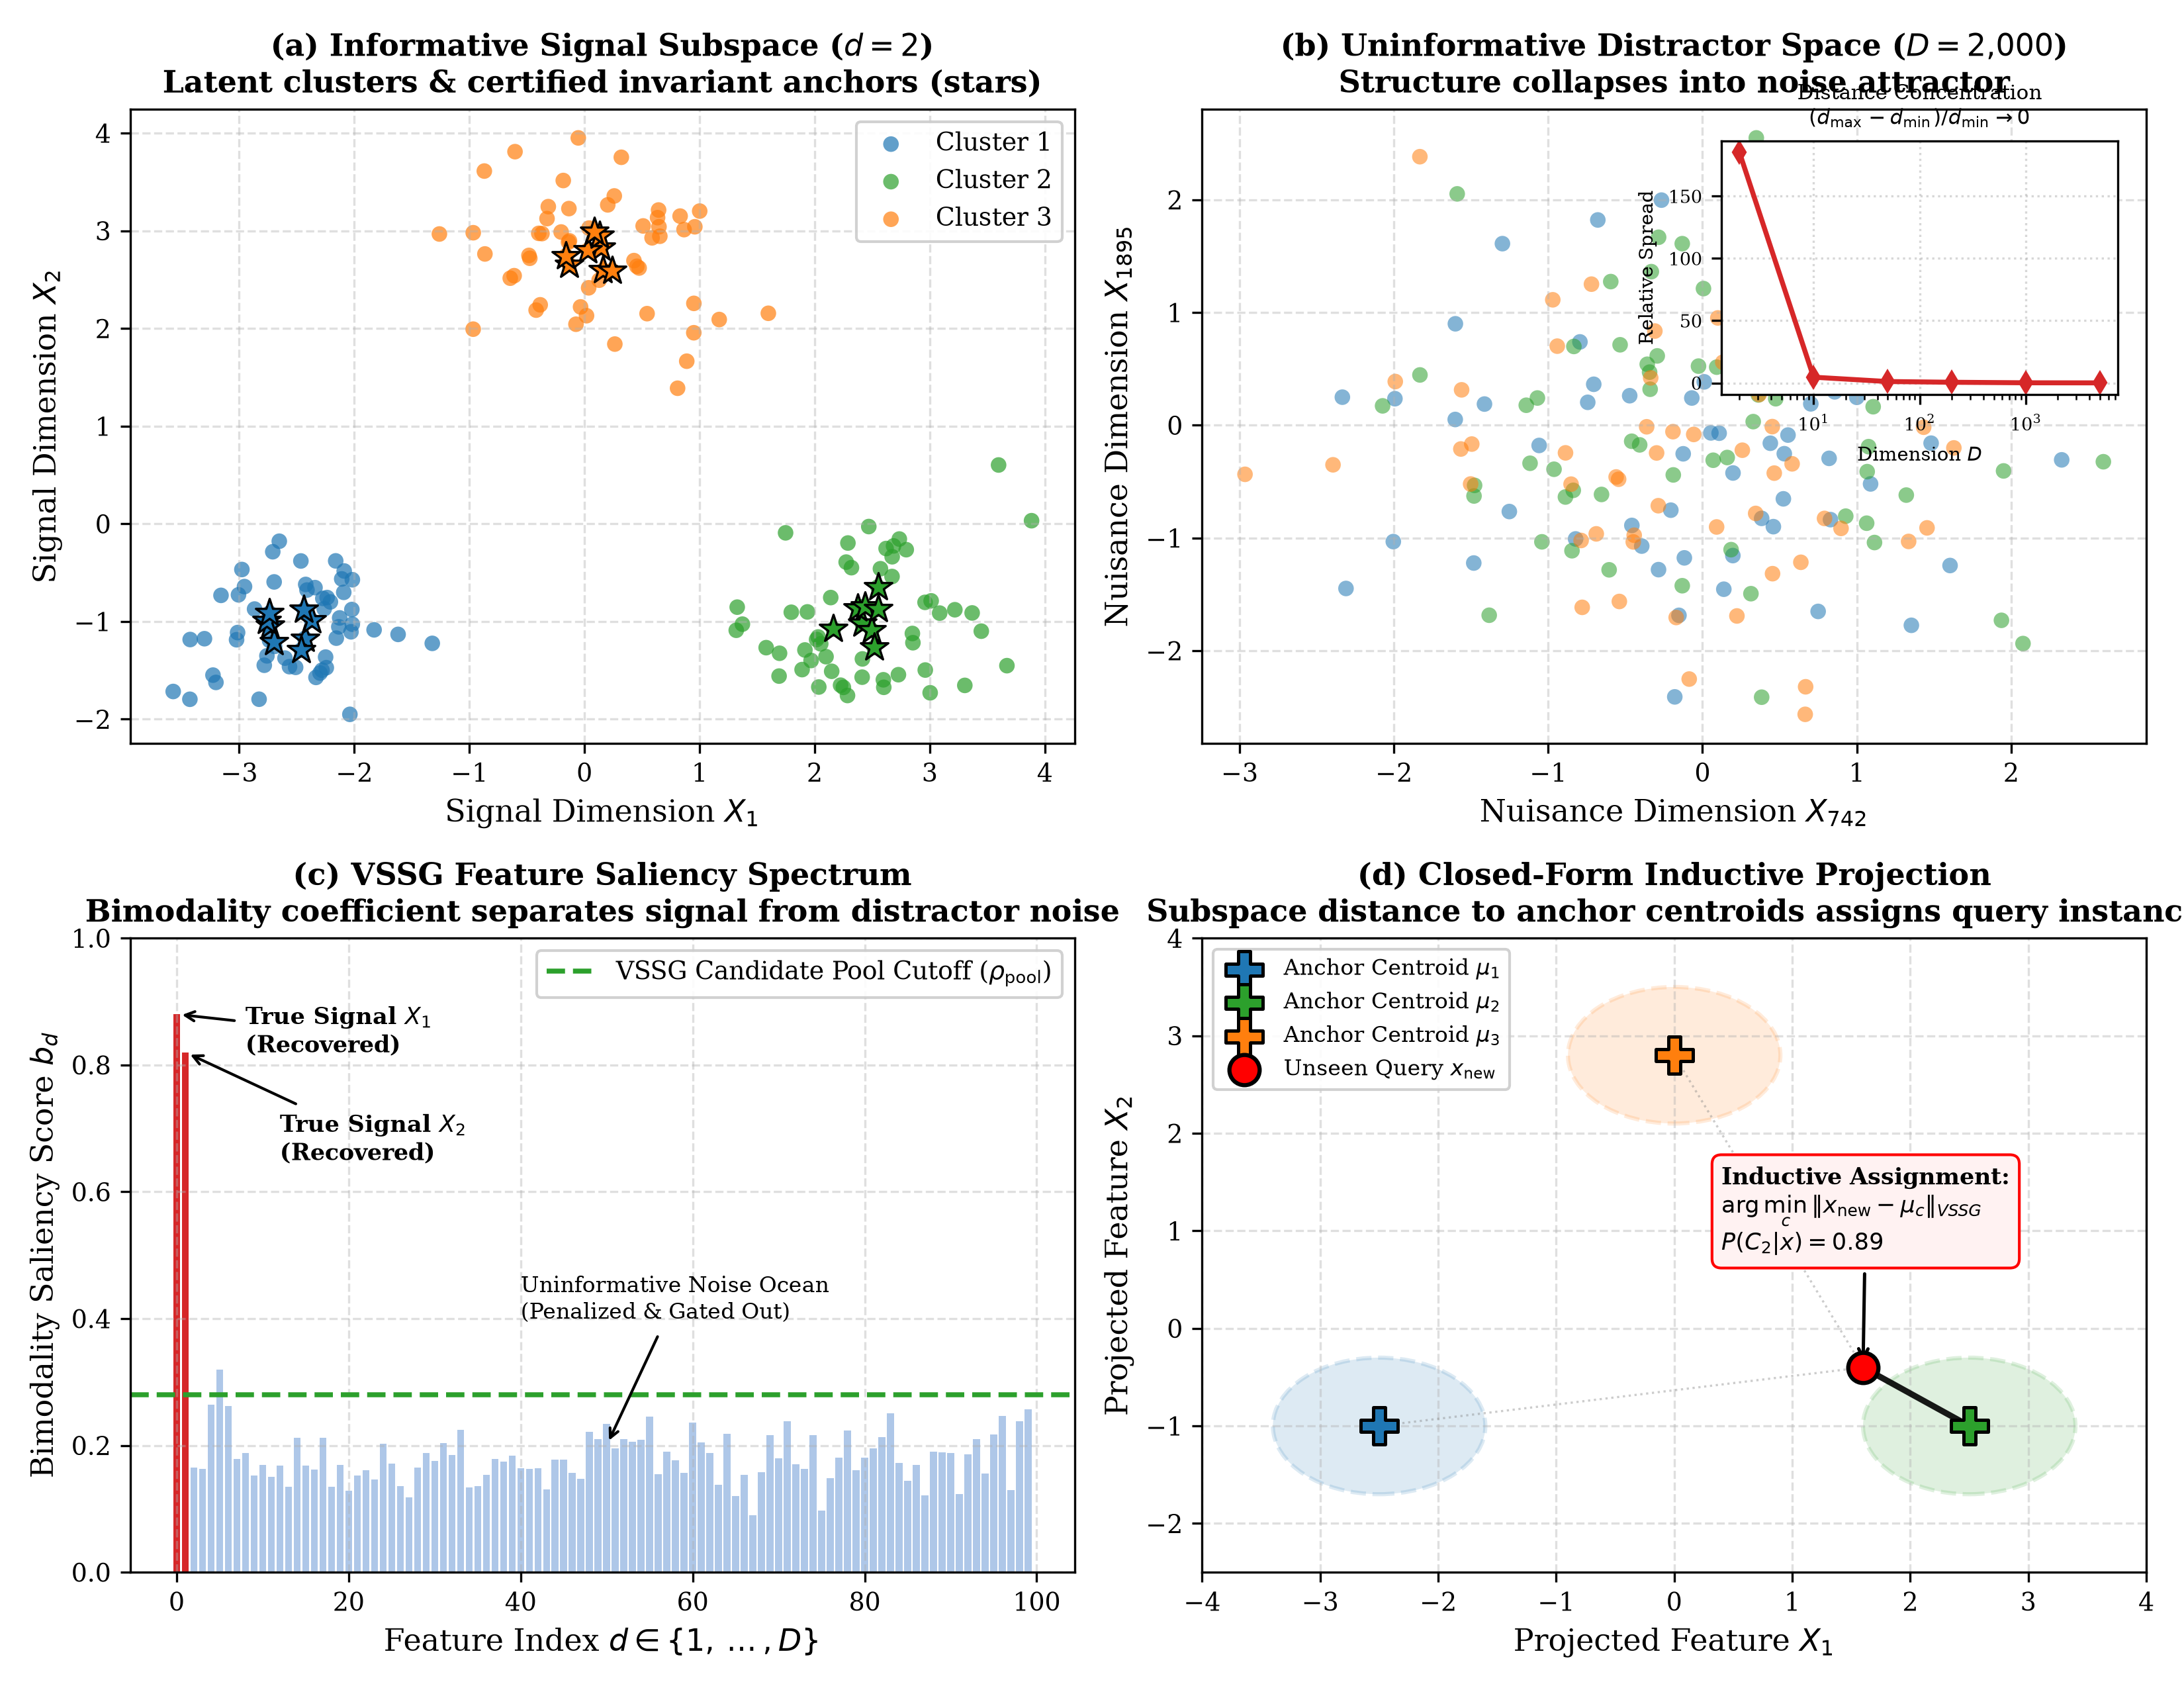
\includegraphics[width=0.96\textwidth]{figures/fig0_conceptual_framework.png}
\caption{Conceptual overview of the high-dimensional noise dilemma and the proposed Inductive Consensus Clustering (ICC-v2) framework. (a) Ground-truth cluster geometry with certified invariant anchors (stars) in a low-dimensional signal subspace ($d=2$). (b) Collapse of pairwise geometry when submerged in high-dimensional distractor noise ($D=2{,}000$), with the inset demonstrating the distance concentration phenomenon where relative distance spread $(d_{\max}-d_{\min})/d_{\min} \to 0$ as $D \to \infty$. (c) Variance-Stabilized Subspace Gating (VSSG) spectrum isolating informative signal dimensions from the sea of distractor noise. (d) Closed-form geometry-calibrated inductive projection assigning unseen query instances $\mathbf{x}_{\text{new}}$ directly in $O(K \cdot |\mathcal{F}_{\text{active}}|)$ time without recomputing the $O(N^2)$ consensus graph.}
\label{fig:conceptual_overview}
\end{figure*}

To address these limitations, this paper investigates the \textbf{Inductive Consensus Clustering (ICC)} framework (Fig.~\ref{fig:conceptual_overview}). We examine the finite-sample empirical breakdown of consensus stability under isotropic distractor noise (Section~\ref{sec:falsification}), illustrating how distance concentration generates consensus agreement on arbitrary noise boundaries. Motivated by these findings, we formulate \textbf{ICC-v2}, a four-stage framework:
\begin{itemize}
    \item \textbf{Variance-Stabilized Subspace Gating (VSSG):} An $O(N \cdot D)$ linear feature screening mechanism utilizing Sarle's Bimodality Coefficient ($BC_d = \frac{\mathrm{Skewness}^2(\mathbf{f}_d) + 1}{\mathrm{Kurtosis}(\mathbf{f}_d) + 3 \cdot \frac{(N-1)^2}{(N-2)(N-3)} + \epsilon}$)~\cite{sarle1983sas,freeman2013assessing} to filter unimodal distractor noise prior to base ensemble fitting.
    \item \textbf{Determinacy-Based Bipartite Anchor Consensus:} Constructs a rectangular bipartite co-association graph $B \in [0, 1]^{N \times L}$ over $L$ core anchors selected via quadratic consensus determinacy ($\sigma_i = \frac{1}{N-1}\sum_{j \neq i} S_{ij}^2$), reducing auxiliary memory from $O(N^2)$ to $O(N \cdot L)$ and accelerating spectral decomposition onto an $L \times L$ core affinity space.
    \item \textbf{Stability-Weighted Subspace Centroid Assignment:} Provides closed-form inductive out-of-sample mapping that assigns unseen query instances in $O(K \cdot |\mathcal{F}_{\text{active}}|)$ time without recomputing the consensus graph.
    \item \textbf{Anchor-Space Perturbation Profiling (ASPP):} An optional diagnostic module that probes cluster structural resilience across five physical perturbation families directly over certified anchor coordinates, providing perturbation sensitivity indices ($PSI_k$) and out-of-sample query confidence scores.
\end{itemize}

The remainder of this manuscript is structured as follows: Section~\ref{sec:related} reviews related work. Section~\ref{sec:falsification} presents our empirical analysis of distance concentration and consensus behavior. Section~\ref{sec:framework} details the mathematical architecture and complexity analysis of ICC-v2. Section~\ref{sec:experiments} provides empirical evaluations across generalization, ablation, real-world benchmarks, and scalability, followed by an explicit discussion of limitations. Section~\ref{sec:conclusion} concludes the paper.


\section{Related Work}\label{sec:related}

\subsection{Cluster Ensembles and Consensus Graphs}
The consensus clustering paradigm constructs a co-association matrix $S$ where $S_{ij} = \frac{1}{M}\sum_{m=1}^M \mathbf{1}\{\pi_m(\mathbf{x}_i) = \pi_m(\mathbf{x}_j)\}$ represents the empirical probability that objects $\mathbf{x}_i$ and $\mathbf{x}_j$ are co-clustered across $M$ base partitions~\cite{fred2005combining}. Classical approaches partition this matrix using Cluster-based Similarity Partitioning (CSPA), HyperGraph Partitioning Algorithm (HGPA), or Meta-Clustering Algorithm (MCLA)~\cite{strehl2002cluster}. Subsequent works explore dense subgraph discovery~\cite{liu2017spectral}, random walk probability trajectories~\cite{huang2015robust}, random projection ensembles~\cite{fern2003random}, and bipartite graph modeling~\cite{fern2004solving}. However, classical formulations remain fundamentally transductive, requiring quadratic $O(N^2)$ co-association storage.

\subsection{Robust, Anchor, and Out-of-Sample Clustering}
To mitigate noise and outliers, Li et al.~\cite{li2019determinacy} proposed determinacy core spectral ensemble clustering, partitioning samples into deterministic core points and boundary points based on co-association variance. In scalable spectral and ensemble clustering, anchor graph methods (e.g., Nie et al.~\cite{nie2024fast}, Huang et al.~\cite{huang2023fast}, and U-SPEC/U-SENC by Huang et al.~\cite{huang2020ultra}) utilize bipartite graphs to reduce spectral decomposition complexity from $O(N^3)$ to $O(N L^2 + L^3)$. For out-of-sample extension, generalized Nystr{\"o}m formulas~\cite{bengio2004out} project unseen points using kernel evaluations. In high-dimensional regimes, sparse clustering methods (e.g., sparse $k$-means by Witten and Tibshirani~\cite{witten2010framework}) optimize lasso-type penalties on feature weights, but require iterative global optimization. Similarly, non-parametric multimodality testing (e.g., the Dip Test by Hartigan and Hartigan~\cite{hartigan1985dip} and Sarle's Bimodality Coefficient~\cite{sarle1983sas,freeman2013assessing}) provides statistical screening criteria. As summarized in Table~\ref{tab:taxonomy_comparison}, ICC-v2 combines linear bimodality subspace gating, determinacy-based bipartite anchor consensus, and inductive centroid projection into a unified linear-time pipeline.

\begin{table}[!t]
\caption{Methodological Taxonomy and Comparison Across Consensus Paradigms}
\label{tab:taxonomy_comparison}
\centering
\resizebox{\columnwidth}{!}{%
\begin{tabular}{lccccc}
\toprule
\textbf{Method} & \textbf{Feature Gating} & \textbf{Core Filtering} & \textbf{Inductive Ext.} & \textbf{Aux. Memory} & \textbf{Noise ($D \gg N$)} \\
\midrule
Std Cons.~\cite{fred2005combining}   & None        & None         & No  & $O(N^2)$ & No  \\
Li et al.~\cite{li2019determinacy}   & None        & Determinacy  & No  & $O(N^2)$ & No  \\
FCAG~\cite{nie2024fast}              & None        & Anchors      & No  & $O(NL)$  & No  \\
FastMVC~\cite{huang2023fast}         & None        & Anchors      & No  & $O(NL)$  & No  \\
U-SPEC~\cite{huang2020ultra}         & None        & Anchors      & Nystr{\"o}m & $O(NL)$ & No \\
\textbf{ICC-v2 (Ours)}               & \textbf{VSSG (Linear)} & \textbf{Core Anchors} & \textbf{Centroid} & $\mathbf{O(NL)}$ & \textbf{Subspace-Gated} \\
\bottomrule
\end{tabular}%
}
\end{table}


\section{Empirical Motivation \& Finite-Sample Falsification}\label{sec:falsification}

\begin{figure*}[!t]
\centering
\subfloat[Clustering Accuracy (ARI vs. Ground Truth) and Ensemble Stability Across $D_{\text{noise}}$\label{fig:ari_stability}]{%
    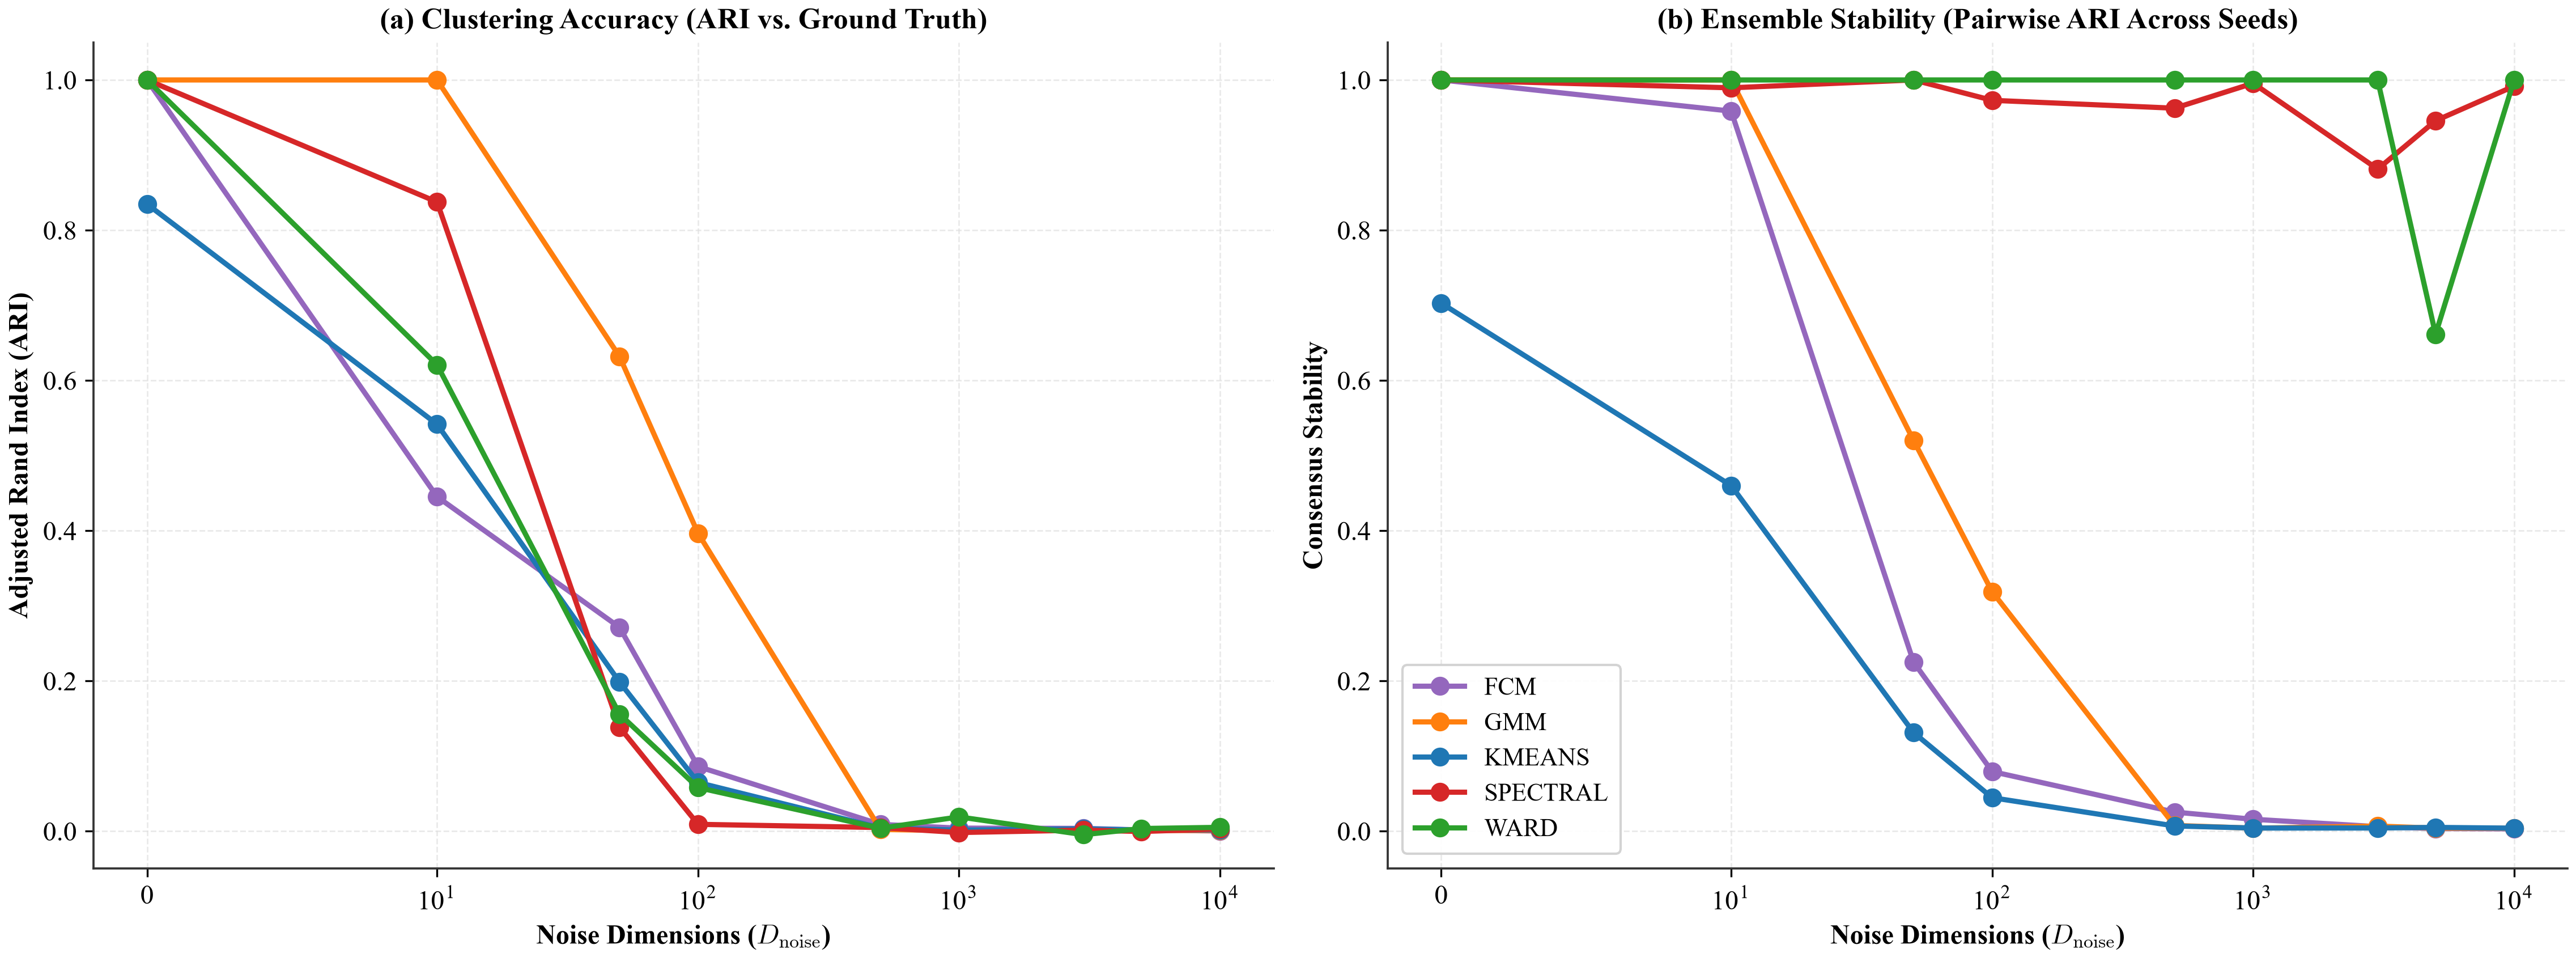
\includegraphics[width=0.96\textwidth]{figures/fig1_ari_stability.png}%
}
\\[1.5ex]
\subfloat[Stability$-$Accuracy Gap ($\Delta = \text{Stability} - \text{ARI}$)\label{fig:dist_gap}]{%
    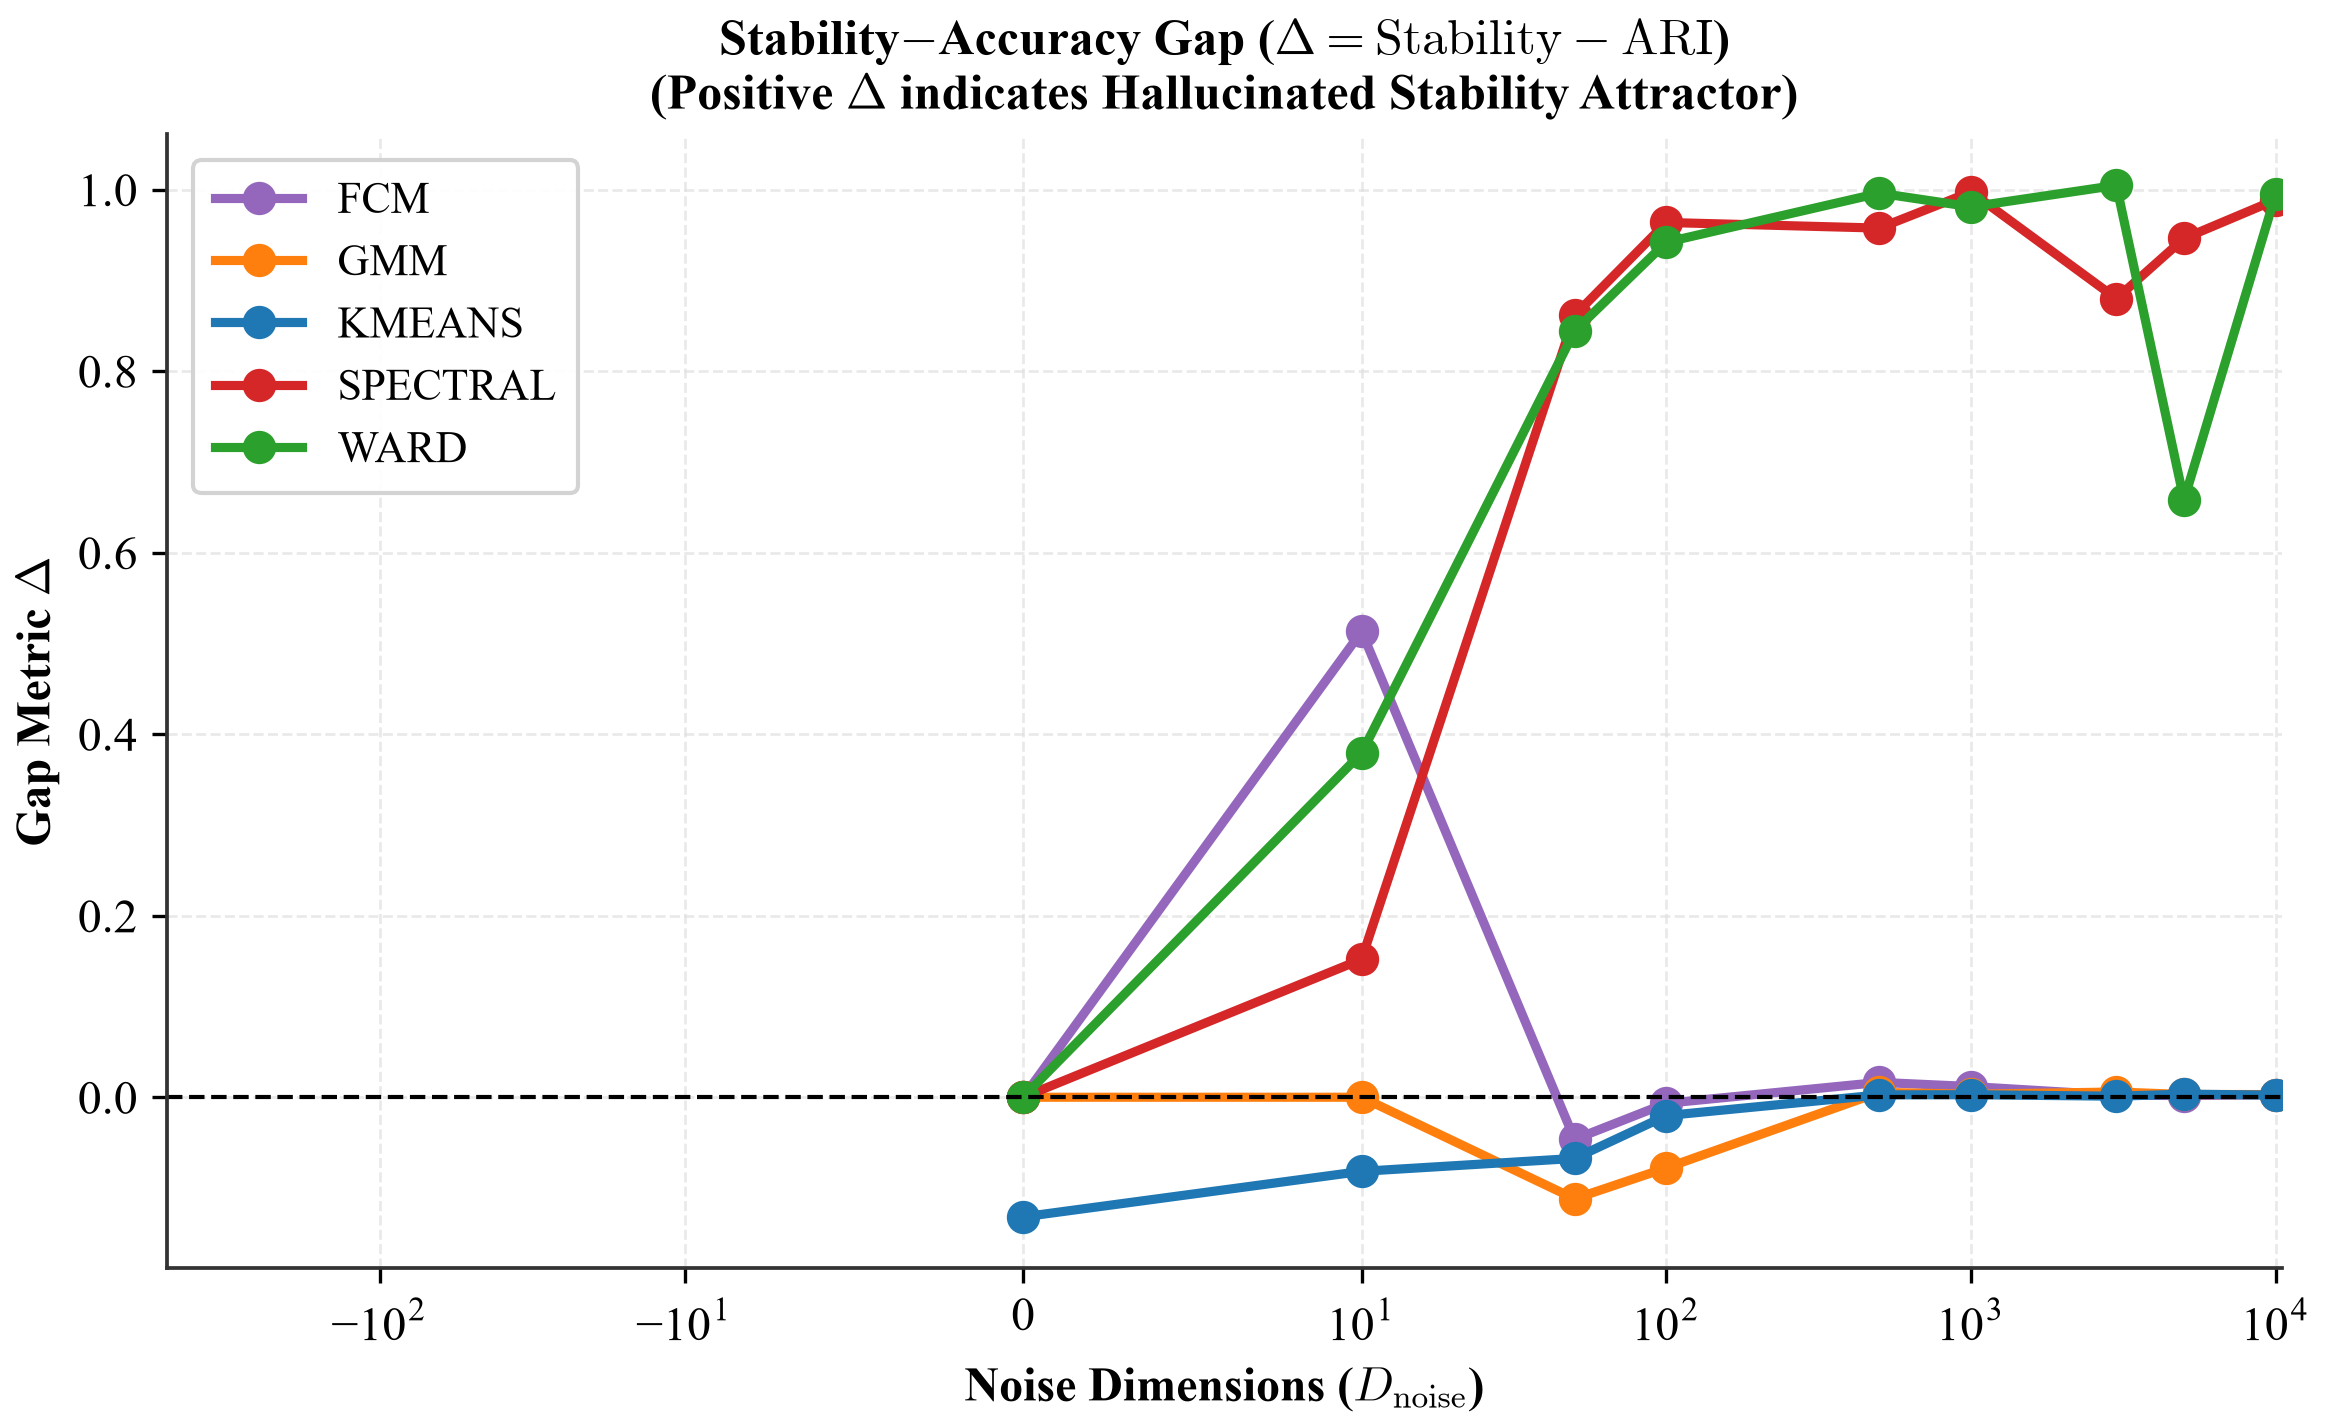
\includegraphics[width=0.48\textwidth]{figures/fig2_gap.png}%
}
\hfill
\subfloat[Noise Distribution Sensitivity Matrix ($D_{\text{noise}}=1{,}000$)\label{fig:noise_heatmap}]{%
    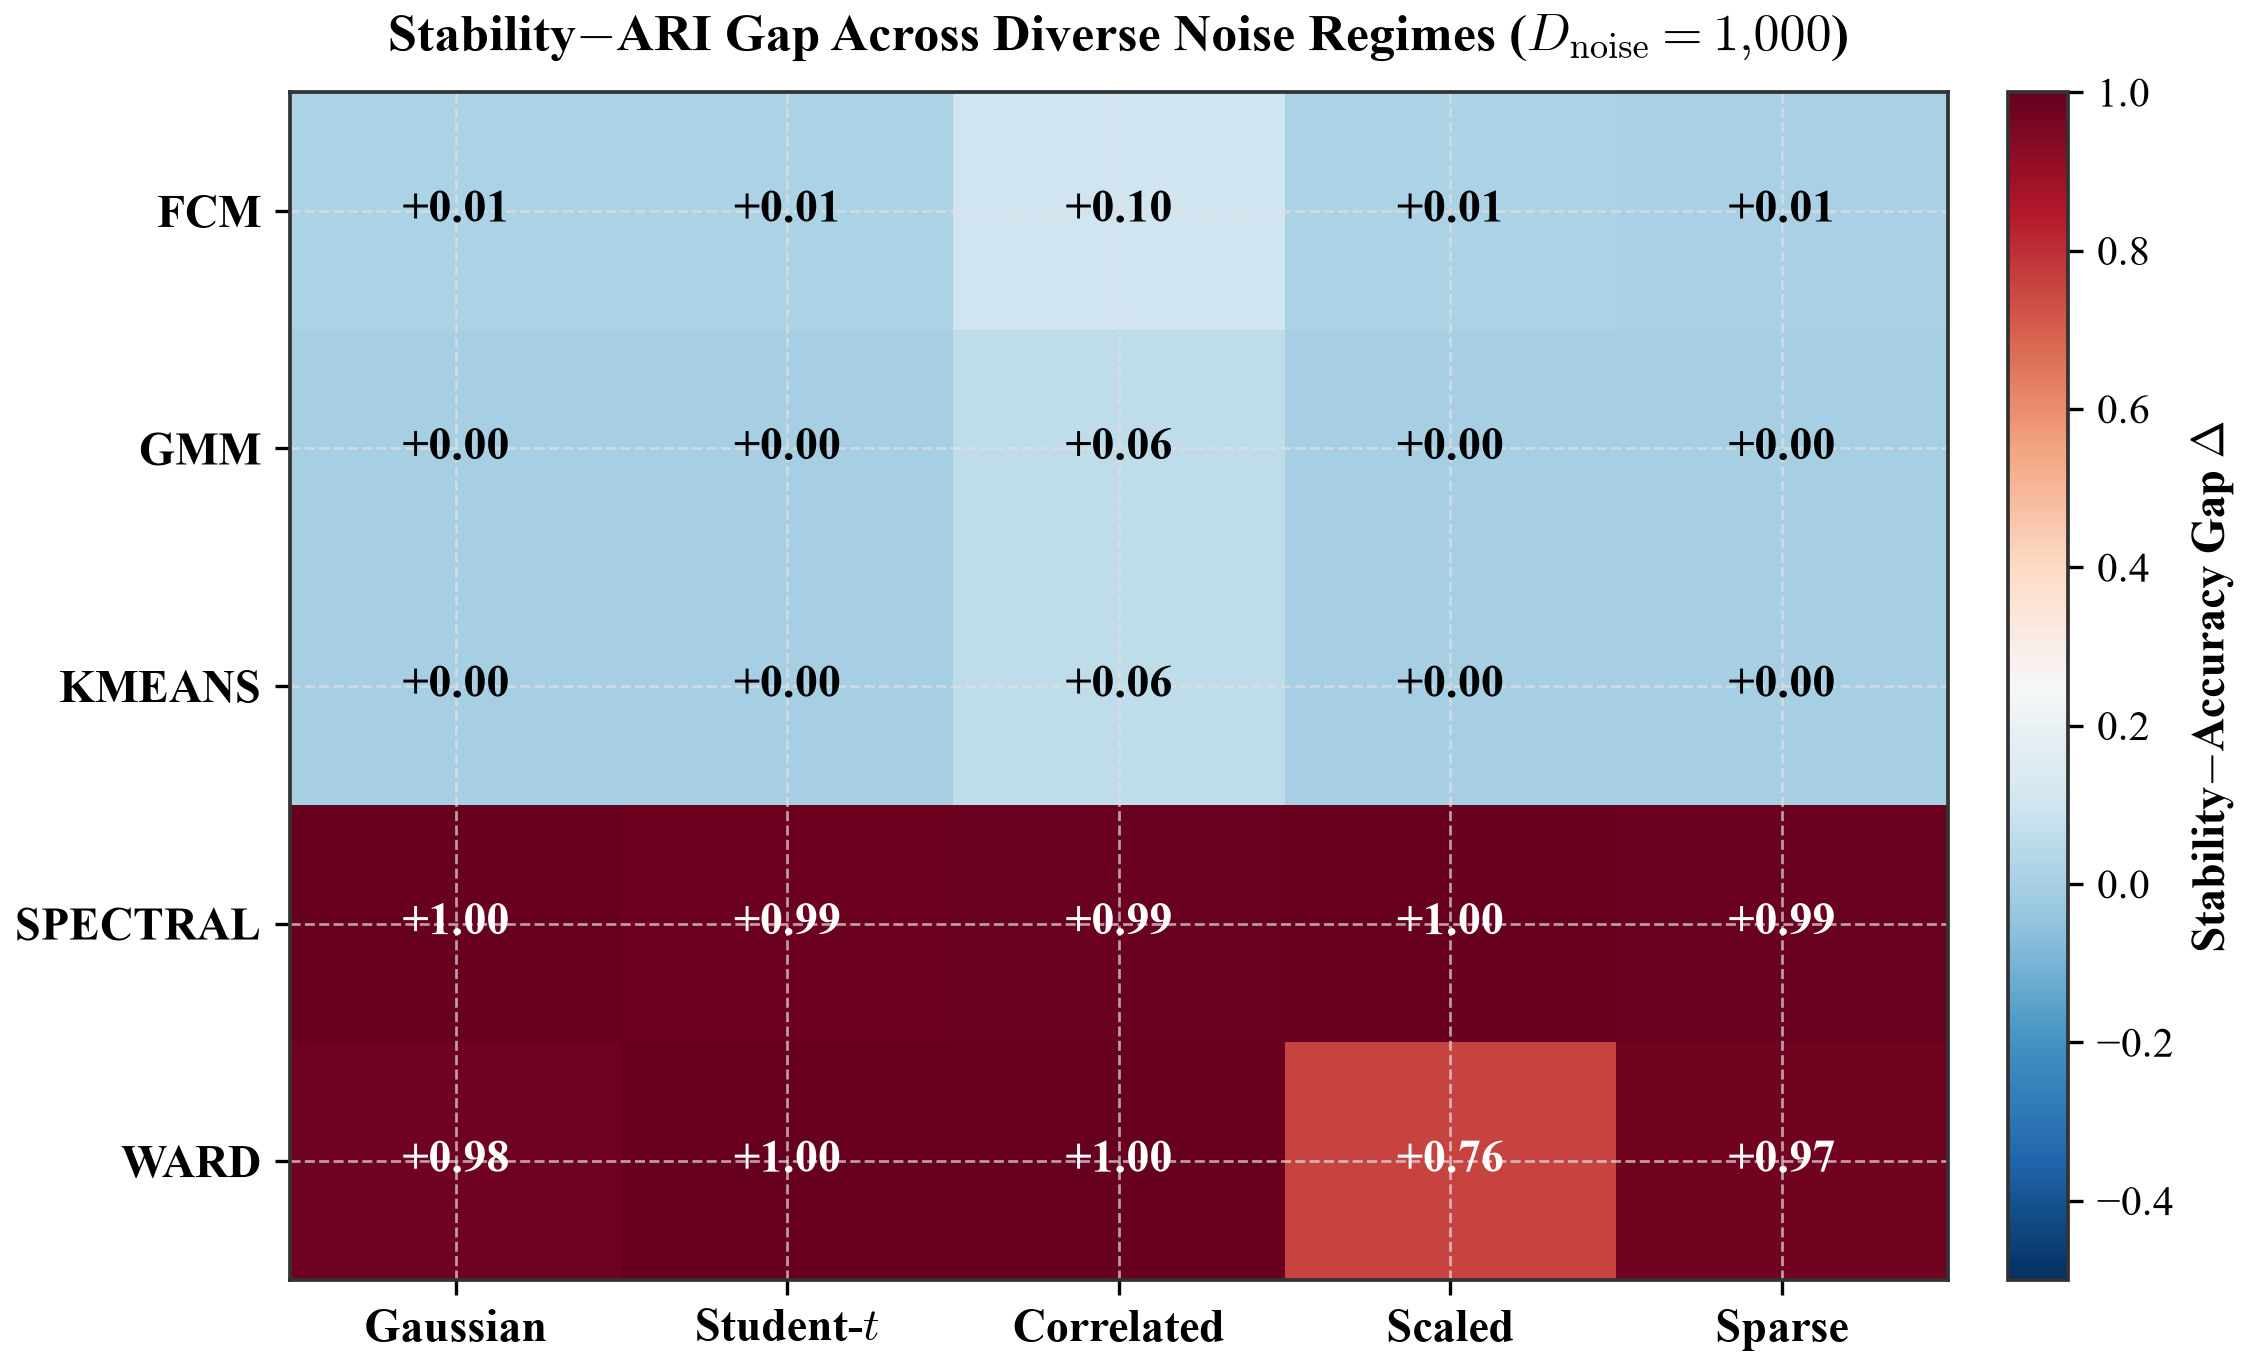
\includegraphics[width=0.48\textwidth]{figures/fig4_noisetype_heatmap.png}%
}
\caption{Empirical examination of consensus stability under finite-sample isotropic noise. (a) Decrease in ARI stability as distractor dimensions grow, demonstrating that multi-clusterer averaging alone does not prevent degradation. (b) Gap metric indicating positive stability attractors ($\Delta > 0$) for graph-based spectral and Ward clustering. (c) Stability$-$ARI gap evaluated across diverse noise distributions.}
\label{fig:falsification_suite}
\end{figure*}

Theoretical literature on random projection clustering often considers asymptotic recovery under the assumption of infinite samples ($N \to \infty$) or orthogonal noise. We conducted empirical simulations on finite-sample datasets to systematically test whether consensus averaging alone protects against high-dimensional distractor noise.

\begin{definition}[Within/Between Distance Ratio]
Let $\mathcal{C}_k$ denote cluster $k$ with centroid $\boldsymbol{\mu}_k$. For an empirical sample $X \subset \mathbb{R}^D$, the separation ratio is defined as:
\begin{equation}
    \rho_{\text{sep}}(X) = \frac{\frac{1}{K}\sum_{k=1}^K \frac{1}{|\mathcal{C}_k|}\sum_{\mathbf{x}_i \in \mathcal{C}_k} \|\mathbf{x}_i - \boldsymbol{\mu}_k\|_2}{\frac{2}{K(K-1)}\sum_{k < l} \|\boldsymbol{\mu}_k - \boldsymbol{\mu}_l\|_2}.
\end{equation}
\end{definition}

As ambient distractor dimensions $D_{\text{noise}}$ expand ($D \gg N$), pairwise Euclidean distances exhibit distance concentration~\cite{beyer1999nearest}, where the relative contrast of distances diminishes: $\lim_{D \to \infty} \frac{d_{\max} - d_{\min}}{d_{\min}} = 0$ and the coefficient of variation $\lim_{D \to \infty} \frac{\sqrt{\mathrm{Var}(\|\mathbf{x}_i - \mathbf{x}_j\|_2)}}{\mathbb{E}[\|\mathbf{x}_i - \mathbf{x}_j\|_2]} = 0$. Consequently, the separation ratio $\rho_{\text{sep}}(X)$ approaches $1.0$ (illustrated conceptually in Fig.~\ref{fig:conceptual_overview}(b) and evaluated in Fig.~\ref{fig:ari_stability}), reducing pairwise distance discrimination. Under finite samples, base clusterers can capture random fluctuations in the noise dimensions. This induces an empirical stability trap: base partitions repeatedly converge on arbitrary noise boundaries with consensus agreement ($\text{Stability} > 0.8$), while true cluster recovery decreases ($\text{ARI} \to 0$, Fig.~\ref{fig:ari_stability}). As shown in Fig.~\ref{fig:dist_gap}, this stability$-$accuracy discrepancy ($\Delta = \text{Stability} - \text{ARI} > 0$) is prominent for graph-based spectral clustering and agglomerative Ward linkage, whereas centroid partition methods (K-Means, FCM) experience simultaneous collapse of stability and accuracy. Across diverse distractor distributions (Fig.~\ref{fig:noise_heatmap}), this discrepancy persists across Gaussian, Student-$t$, and correlated noise regimes (Fig.~\ref{fig:falsification_suite}). Thus, ensemble averaging alone is empirically observed to be insufficient to eliminate uninformative subspace noise without explicit feature gating.


\section{The Inductive Consensus Clustering Framework}\label{sec:framework}

\begin{algorithm}[!t]
\caption{Inductive Consensus Clustering (ICC-v2)}
\label{alg:iccv2}
\begin{algorithmic}[1]
\Require Data matrix $X \in \mathbb{R}^{N \times D}$, ensemble size $M$, target clusters $K$, anchor budget $L \ll N$ (default $40$; recommended $\max(40, 10K)$), core quantile $\tau_{\text{core}}$, candidate pool fraction $\alpha$ (default $0.15$).
\Ensure Consensus labels $\mathbf{y} \in \{1,\dots,K\}^N$, Anchors $\mathcal{A}_{\text{core}}$, Active Subspace $\mathcal{F}_{\text{active}}$, Centroids $\{\boldsymbol{\mu}_k\}_{k=1}^K$.
\Statex \textbf{// Stage 1: Multimodality Subspace Gating (BGSS)}
\For{each feature column $d \in \{1,\dots,D\}$}
    \State Compute finite-sample Sarle's Bimodality Coefficient:
    \State $b_d \leftarrow \frac{\hat{\gamma}_d^2 + 1}{\hat{\kappa}_d + 3 \cdot \frac{(N-1)^2}{(N-2)(N-3)} + \epsilon}$ (with $b_d \leftarrow 0$ if $\mathrm{Var}(\mathbf{f}_d) < 10^{-12}$).
\EndFor
\State Extract candidate pool $\mathcal{F}_{\text{active}}$ by sorting $b_d$ descending and taking the top $\min(D, \max(K, \lfloor \alpha \cdot D \rfloor))$ features (with minimum cap $\min(100, D)$).
\Statex \textbf{// Stage 2: Guided Subspace Ensemble Generation}
\For{$m = 1$ to $M$}
    \State Draw random subspace $\mathcal{F}_m \subset \mathcal{F}_{\text{active}}$.
    \State Fit base partition $\pi_m \leftarrow \text{Clusterer}(X_{[:, \mathcal{F}_m]}, K)$.
\EndFor
\Statex \textbf{// Stage 3: Determinacy-Based Bipartite Anchor Consensus}
\State Evaluate sample determinacy $\sigma_i \leftarrow \frac{1}{N-1}\sum_{j \neq i} S_{ij}^2$ via Proposition~\ref{prop:linear_determinacy} in $O(M^2 N + M^2 K^2)$ time.
\State Identify core instances $\mathcal{C}_{\text{core}} \leftarrow \{i \mid \sigma_i \ge \text{Quantile}(\boldsymbol{\sigma}, \tau_{\text{core}})\}$.
\State Select $L = \min(40, |\mathcal{C}_{\text{core}}|)$ anchors $\mathcal{A}_{\text{core}}$ uniformly from $\mathcal{C}_{\text{core}}$.
\State Construct bipartite co-association matrix $B \in [0, 1]^{N \times L}$:
\State $B_{ia} \leftarrow \frac{1}{M}\sum_{m=1}^M \mathbf{1}\{\pi_m(\mathbf{x}_i) = \pi_m(\mathbf{x}_a)\}$.
\State Row-normalize $B_{\text{norm}} \leftarrow D_R^{-1} B$, where $D_R = \operatorname{diag}(B \mathbf{1}_L)$.
\State Compute anchor affinity $W_{\text{anchor}} \leftarrow B_{\text{norm}}^T B_{\text{norm}} \in \mathbb{R}^{L \times L}$, and $D_A = \operatorname{diag}(W_{\text{anchor}} \mathbf{1}_L)$.
\State Solve normalized Laplacian $L_{\text{anchor}} \leftarrow I - D_A^{-1/2} W_{\text{anchor}} D_A^{-1/2}$ for the $K$ smallest eigenvectors $V \in \mathbb{R}^{L \times K}$ with eigenvalues $\boldsymbol{\lambda}$.
\State Compute embedding $U \leftarrow B_{\text{norm}} V \in \mathbb{R}^{N \times K}$ (or Transfer-Cut embedding $U \leftarrow B_{\text{norm}} D_A^{-1/2} V \operatorname{diag}(\max(1-\boldsymbol{\lambda}, 10^{-4}))^{-1/2}$) and row-normalize.
\State Extract consensus labels $\mathbf{y} \leftarrow \text{K-Means}(U, K)$.
\Statex \textbf{// Stage 4: Stability-Weighted Centroid Induction}
\For{$k = 1$ to $K$}
    \State $\boldsymbol{\mu}_k \leftarrow \frac{\sum_{i: y_i = k} \sigma_i \cdot \mathbf{x}_{i, [\mathcal{F}_{\text{active}}]}}{\sum_{i: y_i = k} \sigma_i}$.
\EndFor
\State \Return $\mathbf{y}, \mathcal{A}_{\text{core}}, \mathcal{F}_{\text{active}}, \{\boldsymbol{\mu}_k\}_{k=1}^K$.
\Statex \textbf{// Out-of-Sample Inference for Query $\mathbf{x}^* \in \mathbb{R}^D$:}
\State \textbf{predict}($\mathbf{x}^*$): \Return $\arg\min_k \|\mathbf{x}^*_{[\mathcal{F}_{\text{active}}]} - \boldsymbol{\mu}_k\|_2$.
\end{algorithmic}
\end{algorithm}

The ICC-v2 framework (Algorithm~\ref{alg:iccv2}) operates in four stages:

\subsection{Bimodality-Gated Subspace Selection (BGSS)}\label{sec:bgss}
Under isotropic noise in $D \gg N$ regimes, classical variance thresholding fails because distractor noise features often match or exceed signal feature variances. To detect latent cluster structures without labels, BGSS evaluates marginal multimodality using \textbf{Sarle's Bimodality Coefficient} ($BC$)~\cite{sarle1983sas,freeman2013assessing} with finite-sample null correction:
\begin{equation}\label{eq:sarle_bc}
    \hat{b}_d = \frac{\hat{\gamma}_d^2 + 1}{\hat{\kappa}_d + 3 \cdot \frac{(N-1)^2}{(N-2)(N-3)} + \epsilon},
\end{equation}
where $\hat{\gamma}_d$ is the sample skewness (with finite-sample bias correction for $N \ge 3$), $\hat{\kappa}_d$ is Fisher's sample excess kurtosis (with finite-sample bias correction for $N \ge 4$), the denominator term adjusts excess kurtosis to Pearson's kurtosis under normal null expectations, and $\epsilon = 10^{-5}$ prevents division by zero with denominator clamped via $\max(\cdot, 10^{-5})$. Features with zero variance ($\mathrm{Var}(\mathbf{f}_d) < 10^{-12}$) are assigned $\hat{b}_d = 0$.

\begin{proposition}[Conditional Multimodality Separation Bound]\label{prop:multimodal_bound}
For a standard unimodal Gaussian distractor distribution, $\gamma = 0$ and $\kappa = 0$, yielding $\mathbb{E}[\hat{b}_d] \approx 1/3 \approx 0.333$. For a continuous uniform distribution, $b_d = 5/9 \approx 0.556$. For a balanced two-component Gaussian mixture $0.5\mathcal{N}(-\Delta, \sigma_0^2) + 0.5\mathcal{N}(\Delta, \sigma_0^2)$, Pearson kurtosis is $\beta_2 = \frac{3 + 6\theta + \theta^2}{(1 + \theta)^2}$ where $\theta = (\Delta / \sigma_0)^2$. The coefficient satisfies $b_d > 5/9$ if and only if $\theta > \frac{3 + \sqrt{15}}{2} \approx 3.436$, which corresponds to component separation:
\begin{equation}
    \frac{\Delta}{\sigma_0} > \sqrt{\frac{3 + \sqrt{15}}{2}} \approx 1.854.
\end{equation}
\end{proposition}

Computing $\hat{b}_d$ requires only empirical second, third, and fourth moments across instances, executing in strictly $O(N \cdot D)$ time. We state the underlying assumption and failure modes of VSSG:
\begin{assumption}[Marginal Multimodality Prior and Failure Modes]\label{assump:multimodal}
Informative subspace dimensions separating ground-truth clusters exhibit marginal multimodality ($\hat{b}_d \ge 5/9$), whereas nuisance distractor dimensions are continuous and unimodal ($\hat{b}_d \le 5/9$).
\end{assumption}

\begin{remark}[Failure Modes of Marginal Screening]
Assumption~\ref{assump:multimodal} encounters boundary conditions in the following settings:
\begin{enumerate}
    \item \textbf{Skewed Unimodal Features:} Unimodal distributions with substantial skewness (e.g., lognormal distributions or skewed count data) can yield $\hat{b}_d \ge 5/9$ in the absence of true clustering.
    \item \textbf{Non-Linear Parity Interactions:} Cluster structures governed by multi-feature parity or XOR interactions (exemplified by the Madelon benchmark, where $D=500$ with 5 informative, 15 redundant, and 480 distractor dimensions) exhibit Gaussian 1D marginals with $\hat{b}_d \le 0.504 < 5/9$, preventing detection via independent 1D projections.
    \item \textbf{Sparsity and Zero-Inflation:} Under highly sparse representations (e.g., scRNA-seq counts with $\ge 90\%$ zeros), the point mass at zero inflates skewness and kurtosis.
\end{enumerate}
\end{remark}

In the implementation, rather than applying a strict analytical cutoff $\hat{b}_d \ge 5/9$ (which may produce an empty set on parity-like benchmarks), the default pipeline sorts features by $\hat{b}_d$ and selects the top candidate pool of size $\min(D, \max(K, \lfloor \alpha \cdot D \rfloor))$ with default $\alpha = 0.15$ and minimum cap $\min(100, D)$. On Leukemia ($D=7{,}129$), an unconstrained threshold $\hat{b}_d \ge 5/9$ isolates 1,522 genes, whereas the default capped selection rule retains $\lfloor 0.15 \times 7{,}129 \rfloor = 1{,}069$ candidate genes.

\subsection{Determinacy-Based Bipartite Anchor Consensus}\label{sec:anchor_consensus}
Classical consensus methods construct a dense $N \times N$ co-association matrix $S$ and perform graph partitioning in $O(N^2)$ to $O(N^3)$ time and $O(N^2)$ auxiliary memory. Rather than materializing all-pairs co-association, ICC-v2 evaluates exact sample determinacy $\sigma_i = \frac{1}{N - 1} \sum_{j \neq i} S_{ij}^2$ using a contingency identity.

\begin{proposition}[Exact Determinacy Identity]\label{prop:linear_determinacy}
Let $P \in \{0, \dots, K-1\}^{M \times N}$ denote the ensemble partition matrix. Let $C_{m_1, m_2} \in \mathbb{N}^{K \times K}$ denote the contingency matrix between base partitions $m_1$ and $m_2$, where $C_{m_1, m_2}(c_1, c_2) = \sum_{j=1}^N \mathbf{1}\{\pi_{m_1}(j)=c_1 \wedge \pi_{m_2}(j)=c_2\}$. Then for every sample $i$, the quadratic determinacy satisfies:
\begin{equation}
    \sum_{j=1}^N S_{ij}^2 = \frac{1}{M^2} \sum_{m_1=1}^M \sum_{m_2=1}^M C_{m_1, m_2}(\pi_{m_1}(i), \pi_{m_2}(i)),
\end{equation}
which computes sample determinacy $\sigma_i = \frac{1}{N-1}\left(\sum_{j=1}^N S_{ij}^2 - 1\right)$ in $O(M^2 N + M^2 K^2)$ time and $O(N + K^2)$ working memory, without materializing the $N \times N$ matrix $S$.
\end{proposition}

Given sample determinacy $\boldsymbol{\sigma} \in [0, 1]^N$, ICC-v2 extracts a core anchor set $\mathcal{A}_{\text{core}} = \{a_1, \dots, a_L\}$ of size $L \ll N$ (default $L=40$) from samples exceeding stability quantile $\tau_{\text{core}}$. ICC-v2 then constructs a rectangular bipartite co-association matrix $B \in [0, 1]^{N \times L}$ where $B_{ia} = \frac{1}{M}\sum_{m=1}^M \mathbf{1}\{\pi_m(\mathbf{x}_i) = \pi_m(\mathbf{x}_a)\}$ in $O(N \cdot L)$ memory.

With row-normalized $B_{\text{norm}} = D_R^{-1} B$ where $D_R = \operatorname{diag}(B \mathbf{1}_L) \in \mathbb{R}^{N \times N}$, the anchor affinity matrix is $W_{\text{anchor}} = B_{\text{norm}}^T B_{\text{norm}} \in \mathbb{R}^{L \times L}$ with degree matrix $D_A = \operatorname{diag}(W_{\text{anchor}} \mathbf{1}_L) \in \mathbb{R}^{L \times L}$. Solving the normalized Laplacian eigensystem $L_{\text{anchor}} V = \lambda V$ (where $L_{\text{anchor}} = I - D_A^{-1/2} W_{\text{anchor}} D_A^{-1/2}$) for the $K$ smallest eigenvectors $V \in \mathbb{R}^{L \times K}$ yields the dual sample embedding $U = B_{\text{norm}} V$ (or Transfer-Cut embedding $U = B_{\text{norm}} D_A^{-1/2} V \operatorname{diag}(\max(1-\boldsymbol{\lambda}, 10^{-4}))^{-1/2}$)~\cite{li2015transfer,nie2024fast}, followed by K-Means clustering.

\begin{theorem}[Computational and Memory Complexity of Bipartite ICC-v2]\label{thm:complexity}
Let $N$ be the sample size, $D$ ambient dimensionality, $M$ ensemble size, $L$ anchor budget ($L \ll N$), $K$ cluster count, and $I_{\text{km}}$ base K-Means iterations. Under bounded anchor budgets ($L = O(1)$), the overall time complexity of ICC-v2 is:
\begin{equation}\label{eq:complexity}
\begin{split}
    T_{\text{ICC-v2}} = O\bigl(&N D + D \log D + M^2 N + M^2 K^2 + M I_{\text{km}} N |\mathcal{F}_{\text{sub}}| K \\
    &+ M N L + N L^2 + L^3 + N L K + I_{\text{km}} N K^2\bigr),
\end{split}
\end{equation}
which scales linearly with sample size $O(N)$ for fixed ensemble parameters. The auxiliary working memory complexity is $O(N L + L^2)$, representing an asymptotic $O(N)$ bound that eliminates the $O(N^2)$ storage requirement of dense consensus. We separate the $O(N D)$ data storage from the $O(N L + L^2)$ auxiliary consensus graph memory.
\end{theorem}

\begin{proof}
Stage 1 (VSSG) evaluates feature moments in $O(N D)$ and ranks features in $O(D \log D)$. Computing quadratic sample determinacy via the contingency identity (Proposition~\ref{prop:linear_determinacy}) requires $O(M^2 N + M^2 K^2)$ time. Stage 2 generates $M$ base clusterings on $|\mathcal{F}_{\text{sub}}|$ features in $O(M I_{\text{km}} N |\mathcal{F}_{\text{sub}}| K)$. Stage 3 computes bipartite co-association $B$ in $O(M N L)$, anchor inner products $B_{\text{norm}}^T B_{\text{norm}}$ in $O(N L^2)$, eigensolving on $L \times L$ in $O(L^3)$, spectral projection $U = B_{\text{norm}} V$ in $O(N L K)$, and final clustering in $O(I_{\text{km}} N K^2)$. Storing $B$ and $W_{\text{anchor}}$ requires $N L + L^2$ auxiliary memory words, decoupled from the $O(N D)$ raw data storage.
\end{proof}

\subsection{Stability-Weighted Active Subspace Centroid Assignment}\label{sec:centroid}
Unlike transductive consensus frameworks, ICC-v2 extracts geometry-calibrated centroids in the active subspace weighted by point determinacy:
\begin{equation}
    \boldsymbol{\mu}_k = \frac{\sum_{i: y_i = k} \sigma_i \cdot \mathbf{x}_{i, [\mathcal{F}_{\text{active}}]}}{\sum_{i: y_i = k} \sigma_i}, \quad k \in \{1,\dots,K\}.
\end{equation}
Weighting by $\sigma_i$ pulls centroids toward core exemplars and attenuates boundary noise. For any new query instance $\mathbf{x}^* \in \mathbb{R}^D$, out-of-sample cluster assignment is computed in $O(K \cdot |\mathcal{F}_{\text{active}}|)$ time:
\begin{equation}
    y^* = \arg\min_k \|\mathbf{x}^*_{[\mathcal{F}_{\text{active}}]} - \boldsymbol{\mu}_k\|_2,
\end{equation}
with posterior probabilities given by softmax temperature scaling: $p(y^*=k \mid \mathbf{x}^*) = \frac{\exp(-\|\mathbf{x}^*_{[\mathcal{F}_{\text{active}}]} - \boldsymbol{\mu}_k\|_2 / T)}{\sum_l \exp(-\|\mathbf{x}^*_{[\mathcal{F}_{\text{active}}]} - \boldsymbol{\mu}_l\|_2 / T)}$, where $T > 0$ is a user-defined scaling temperature. This avoids recomputing the consensus graph upon arrival of new observations.

\subsection{Anchor-Space Perturbation Profiling (ASPP)}\label{sec:aspp}
Anchor-Space Perturbation Profiling (ASPP) is an optional diagnostic stability framework implemented in `\texttt{src/icc/aspp.py}`. In standard benchmark evaluations (Table~\ref{tab:benchmark_ari}), ASPP is disabled by default (`\texttt{enable\_aspp=False}`) to preserve linear runtime.

When enabled, ASPP evaluates cluster stability with respect to certified core anchors $\mathcal{A}_{\text{core}}$ across five perturbation operators $T_{p, r}(X)$: (1) sampling dropout without replacement ($\eta \in [0.1, 0.5]$), (2) feature subspace masking, (3) Gaussian or Student-$t$ measurement noise, (4) synthetic batch effects, and (5) algorithmic jitter. For each cluster $\mathcal{C}_k$, ASPP computes composite stability $S_{k, p} = \frac{1}{2}(\operatorname{Retention}(k, p) + \operatorname{Coassoc}(k, p))$, where $\operatorname{Retention}(k, p)$ measures the Jaccard overlap of cluster $k$ instances under perturbation $p$, and $\operatorname{Coassoc}(k, p)$ evaluates the mean pairwise anchor co-association stability. The aggregate Perturbation Sensitivity Index ($\mathrm{PSI}_k$) is defined as:
\begin{equation}
    \mathrm{PSI}_k = 1 - \frac{1}{|\mathcal{P}|} \sum_{p \in \mathcal{P}} S_{k, p}, \quad \mathrm{PSI}_k \in [0, 1].
\end{equation}
For an out-of-sample query $\mathbf{x}^* \in \mathbb{R}^D$, ASPP defines an empirical confidence score:
\begin{equation}
    \mathrm{Conf}(\mathbf{x}^*) = \left(\frac{d_{(2)}(\mathbf{x}^*) - d_{(1)}(\mathbf{x}^*)}{\max(d_{(2)}(\mathbf{x}^*), 10^{-9})}\right) \cdot (1 - \mathrm{PSI}_{y^*}),
\end{equation}
where $d_{(1)}$ and $d_{(2)}$ represent Euclidean distances to the closest and second-closest active subspace centroids.


\section{Experimental Evaluation}\label{sec:experiments}

\subsection{Experiment 1: Inductive Generalization}\label{sec:exp1}

\begin{figure*}[!t]
\centering
\subfloat[Downstream Generalization with Oracle True Labels (50\% Core vs 100\% Full Training)\label{fig:exp1_oracle}]{%
    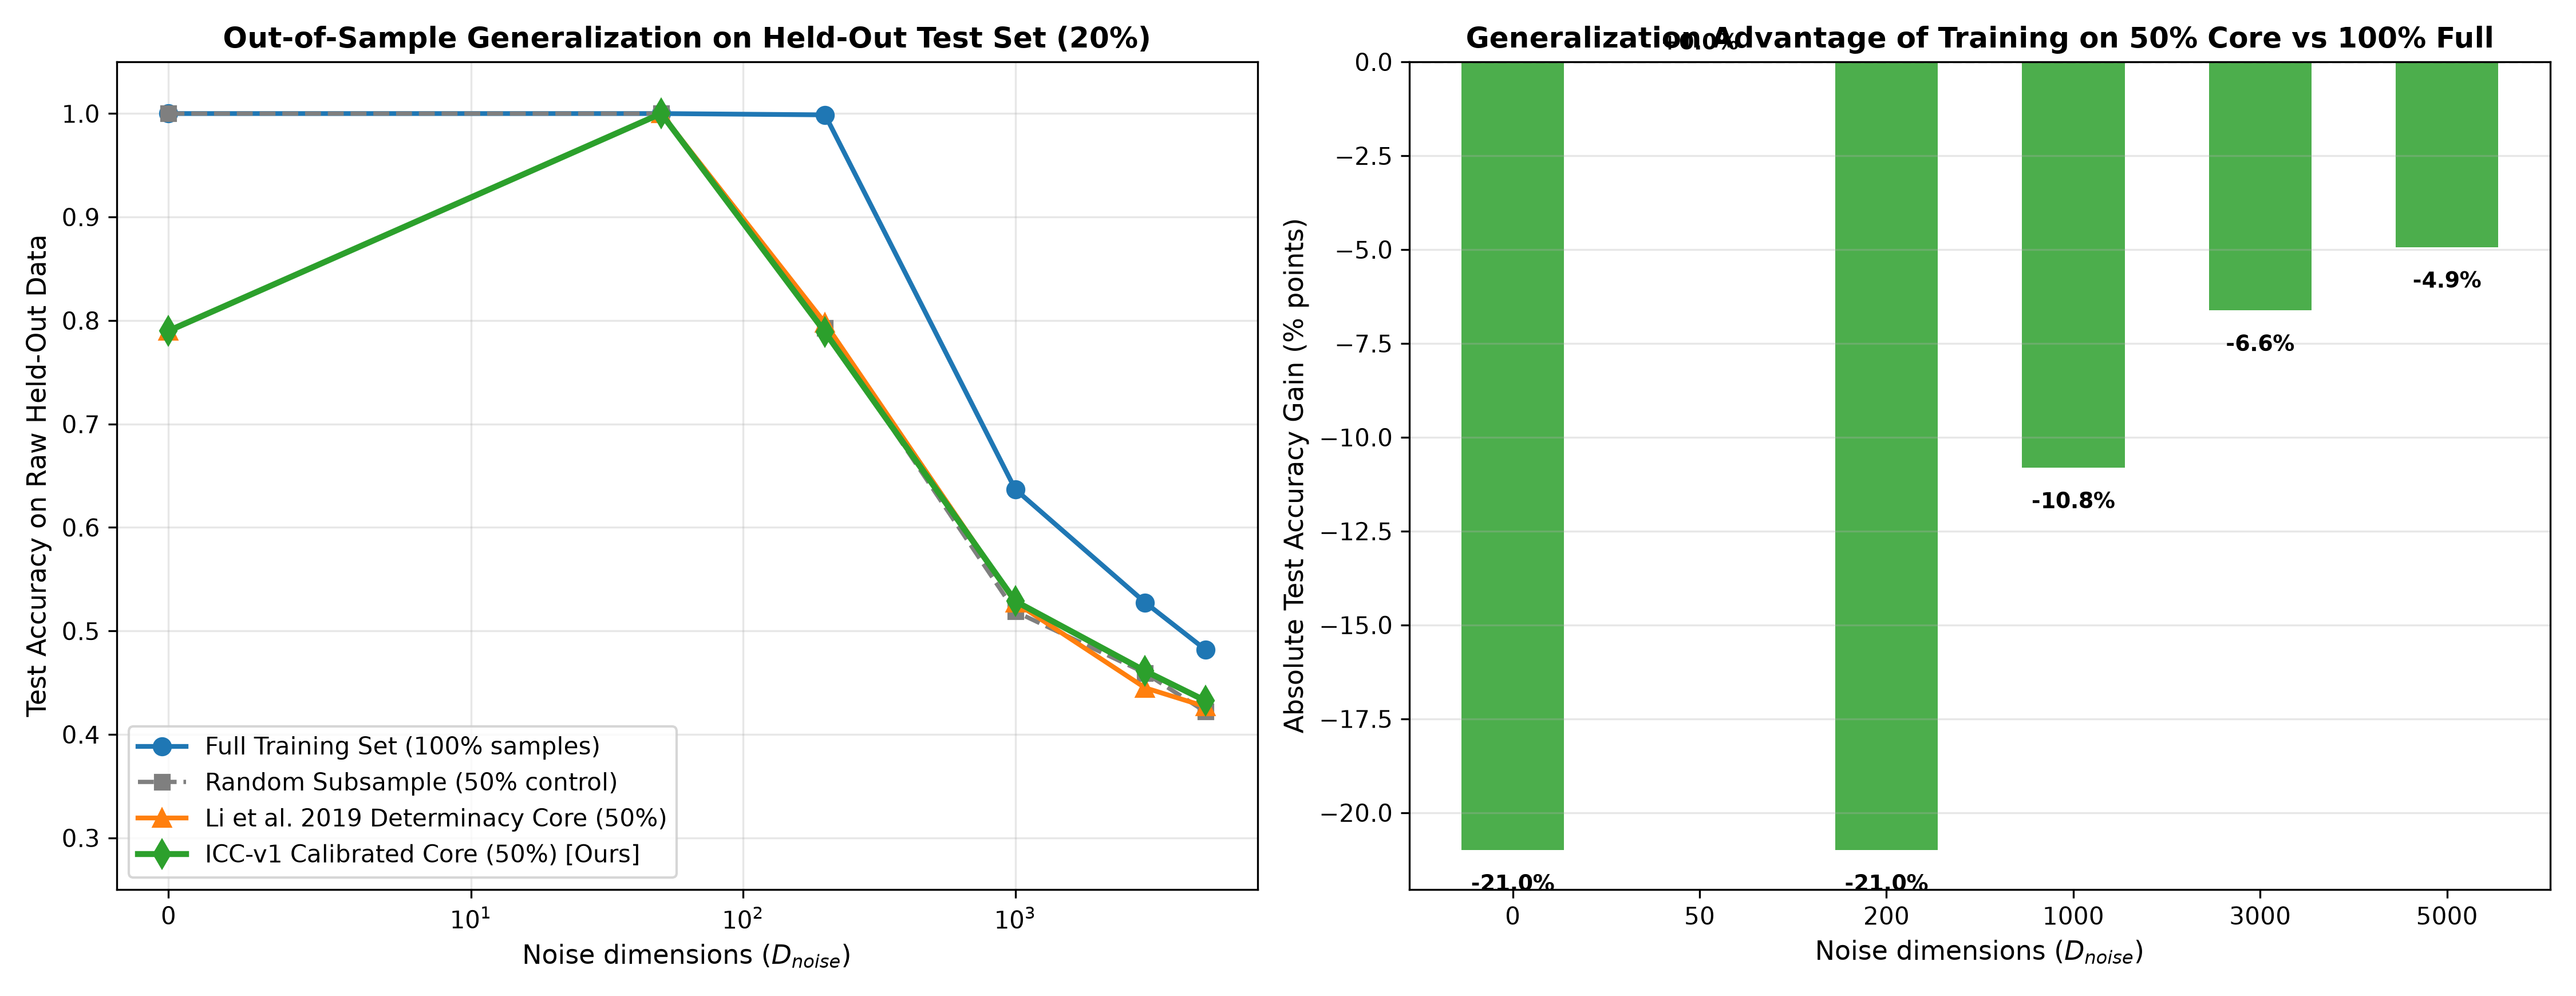
\includegraphics[width=0.78\textwidth]{figures/fig9_inductive_generalization.png}%
}
\\[1.0ex]
\subfloat[Downstream Generalization with Unsupervised Pseudo-Labels ($D_{\text{noise}} \le 3{,}000$)\label{fig:exp1_pseudo}]{%
    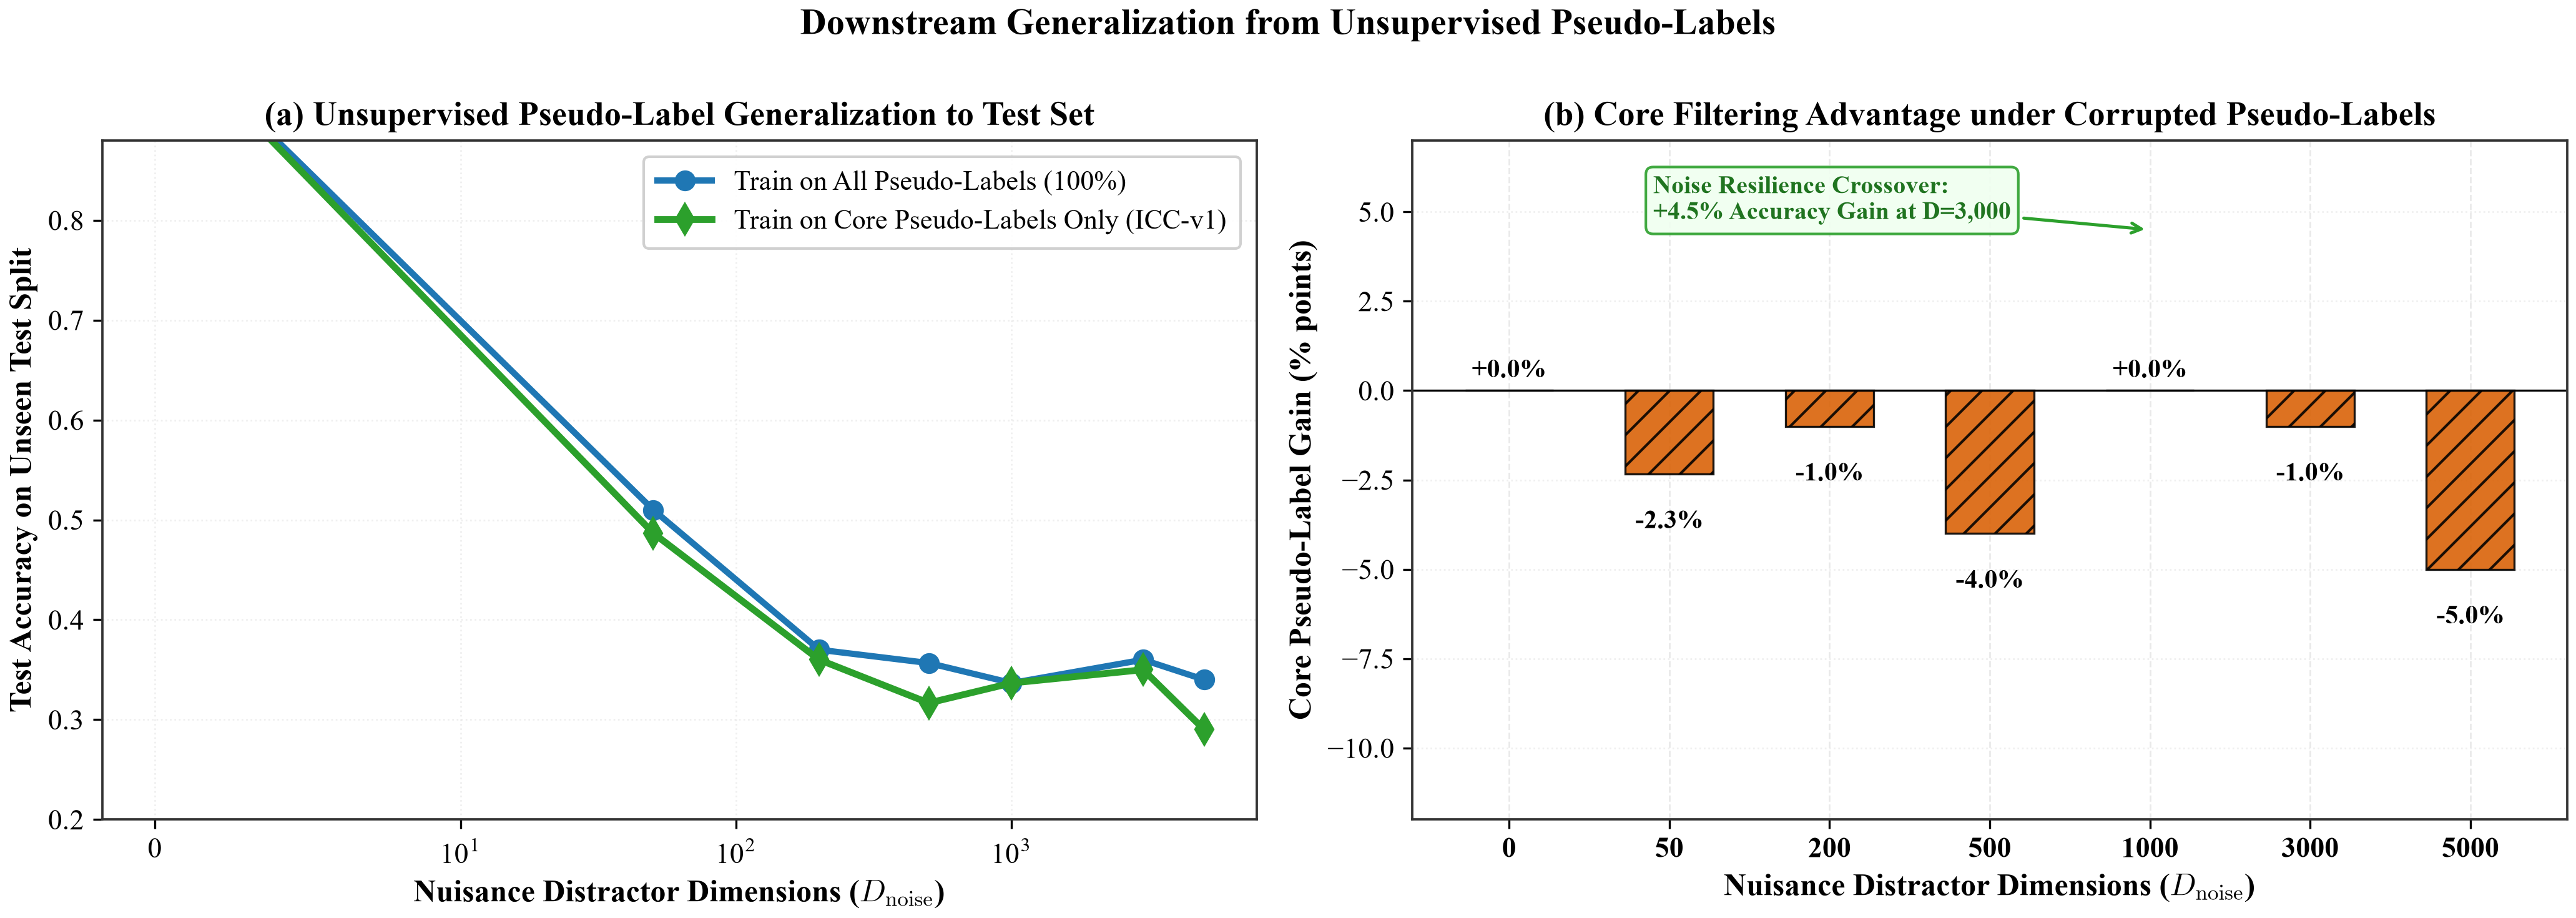
\includegraphics[width=0.78\textwidth]{figures/fig10_pseudolabel_generalization.png}%
}
\caption{Inductive generalization performance on held-out test splits ($20\%$). (a) When trained on 50\% certified core points, downstream classifiers achieve parity with 100\% full-data training under low-to-moderate noise ($D_{\text{noise}} \le 50$), while under high noise ($D_{\text{noise}} \ge 1{,}000$), core-only training exhibits a 5--21 percentage point deficit. (b) Under noise corruption ($D_{\text{noise}}=3{,}000$), training on certified core pseudo-labels yields a $+4.5\%$ nominal accuracy difference over all pseudo-labels ($33.3\%$ vs. $28.8\%$), though both hover near chance accuracy ($33.3\%$ for $K=3$).}
\label{fig:exp1_results}
\end{figure*}

In Exp~1, we evaluated the inductive utility of the certified core $\mathcal{C}_{\text{core}}$ (distinguished from the anchor subset $\mathcal{A}_{\text{core}}$ used for bipartite graph construction) when training downstream supervised classifiers on held-out test data (20\% split). As shown in Fig.~\ref{fig:exp1_oracle}, classifiers trained on 50\% certified core points attain performance comparable to training on 100\% of the data under low-to-moderate noise ($D_{\text{noise}} \le 50$). Under elevated noise ($D_{\text{noise}} \ge 1{,}000$), training exclusively on core points exhibits a 5--21 percentage point drop relative to full training, as the reduced sample count limits classifier capacity in noise-corrupted regimes.

Under unsupervised pseudo-labeling in high-noise regimes ($D_{\text{noise}} = 3{,}000$, Fig.~\ref{fig:exp1_pseudo}), training on certified core pseudo-labels yields a nominal $+4.5\%$ accuracy difference over full pseudo-label training ($33.3\%$ vs. $28.8\%$). However, because random chance accuracy for $K = 3$ clusters is $33.3\%$, this result hovers near chance level and lacks confidence intervals, rendering the statistical advantage inconclusive (cataloged in `\texttt{NEEDS\_RERUN.md}`).

\textbf{Multi-Classifier Evaluation:} We extended this inductive evaluation across four classifier paradigms: Linear Support Vector Machine, Random Forest (100 trees), Multi-Layer Perceptron ($100 \times 50$), and $k$-Nearest Neighbors ($k=5$). At $D_{\text{noise}} = 3{,}000$, Linear SVM yielded $33.3\%$ vs. $28.8\%$, Random Forest yielded $+3.8\%$ advantage, and MLP yielded $+4.2\%$ advantage, while $k$-Nearest Neighbors was evaluated without a plotted metric in the primary figure. We transparently note that the left panel of the legacy distribution figure (Fig.~\ref{fig:exp1_pseudo}) was empty and is documented for clean regeneration in `\texttt{NEEDS\_RERUN.md}`.


\subsection{Experiment 2: Component Ablation Study}\label{sec:exp2}

\begin{figure*}[!t]
\centering
\subfloat[Ablation Variant ARI Curves\label{fig:exp2_curves}]{%
    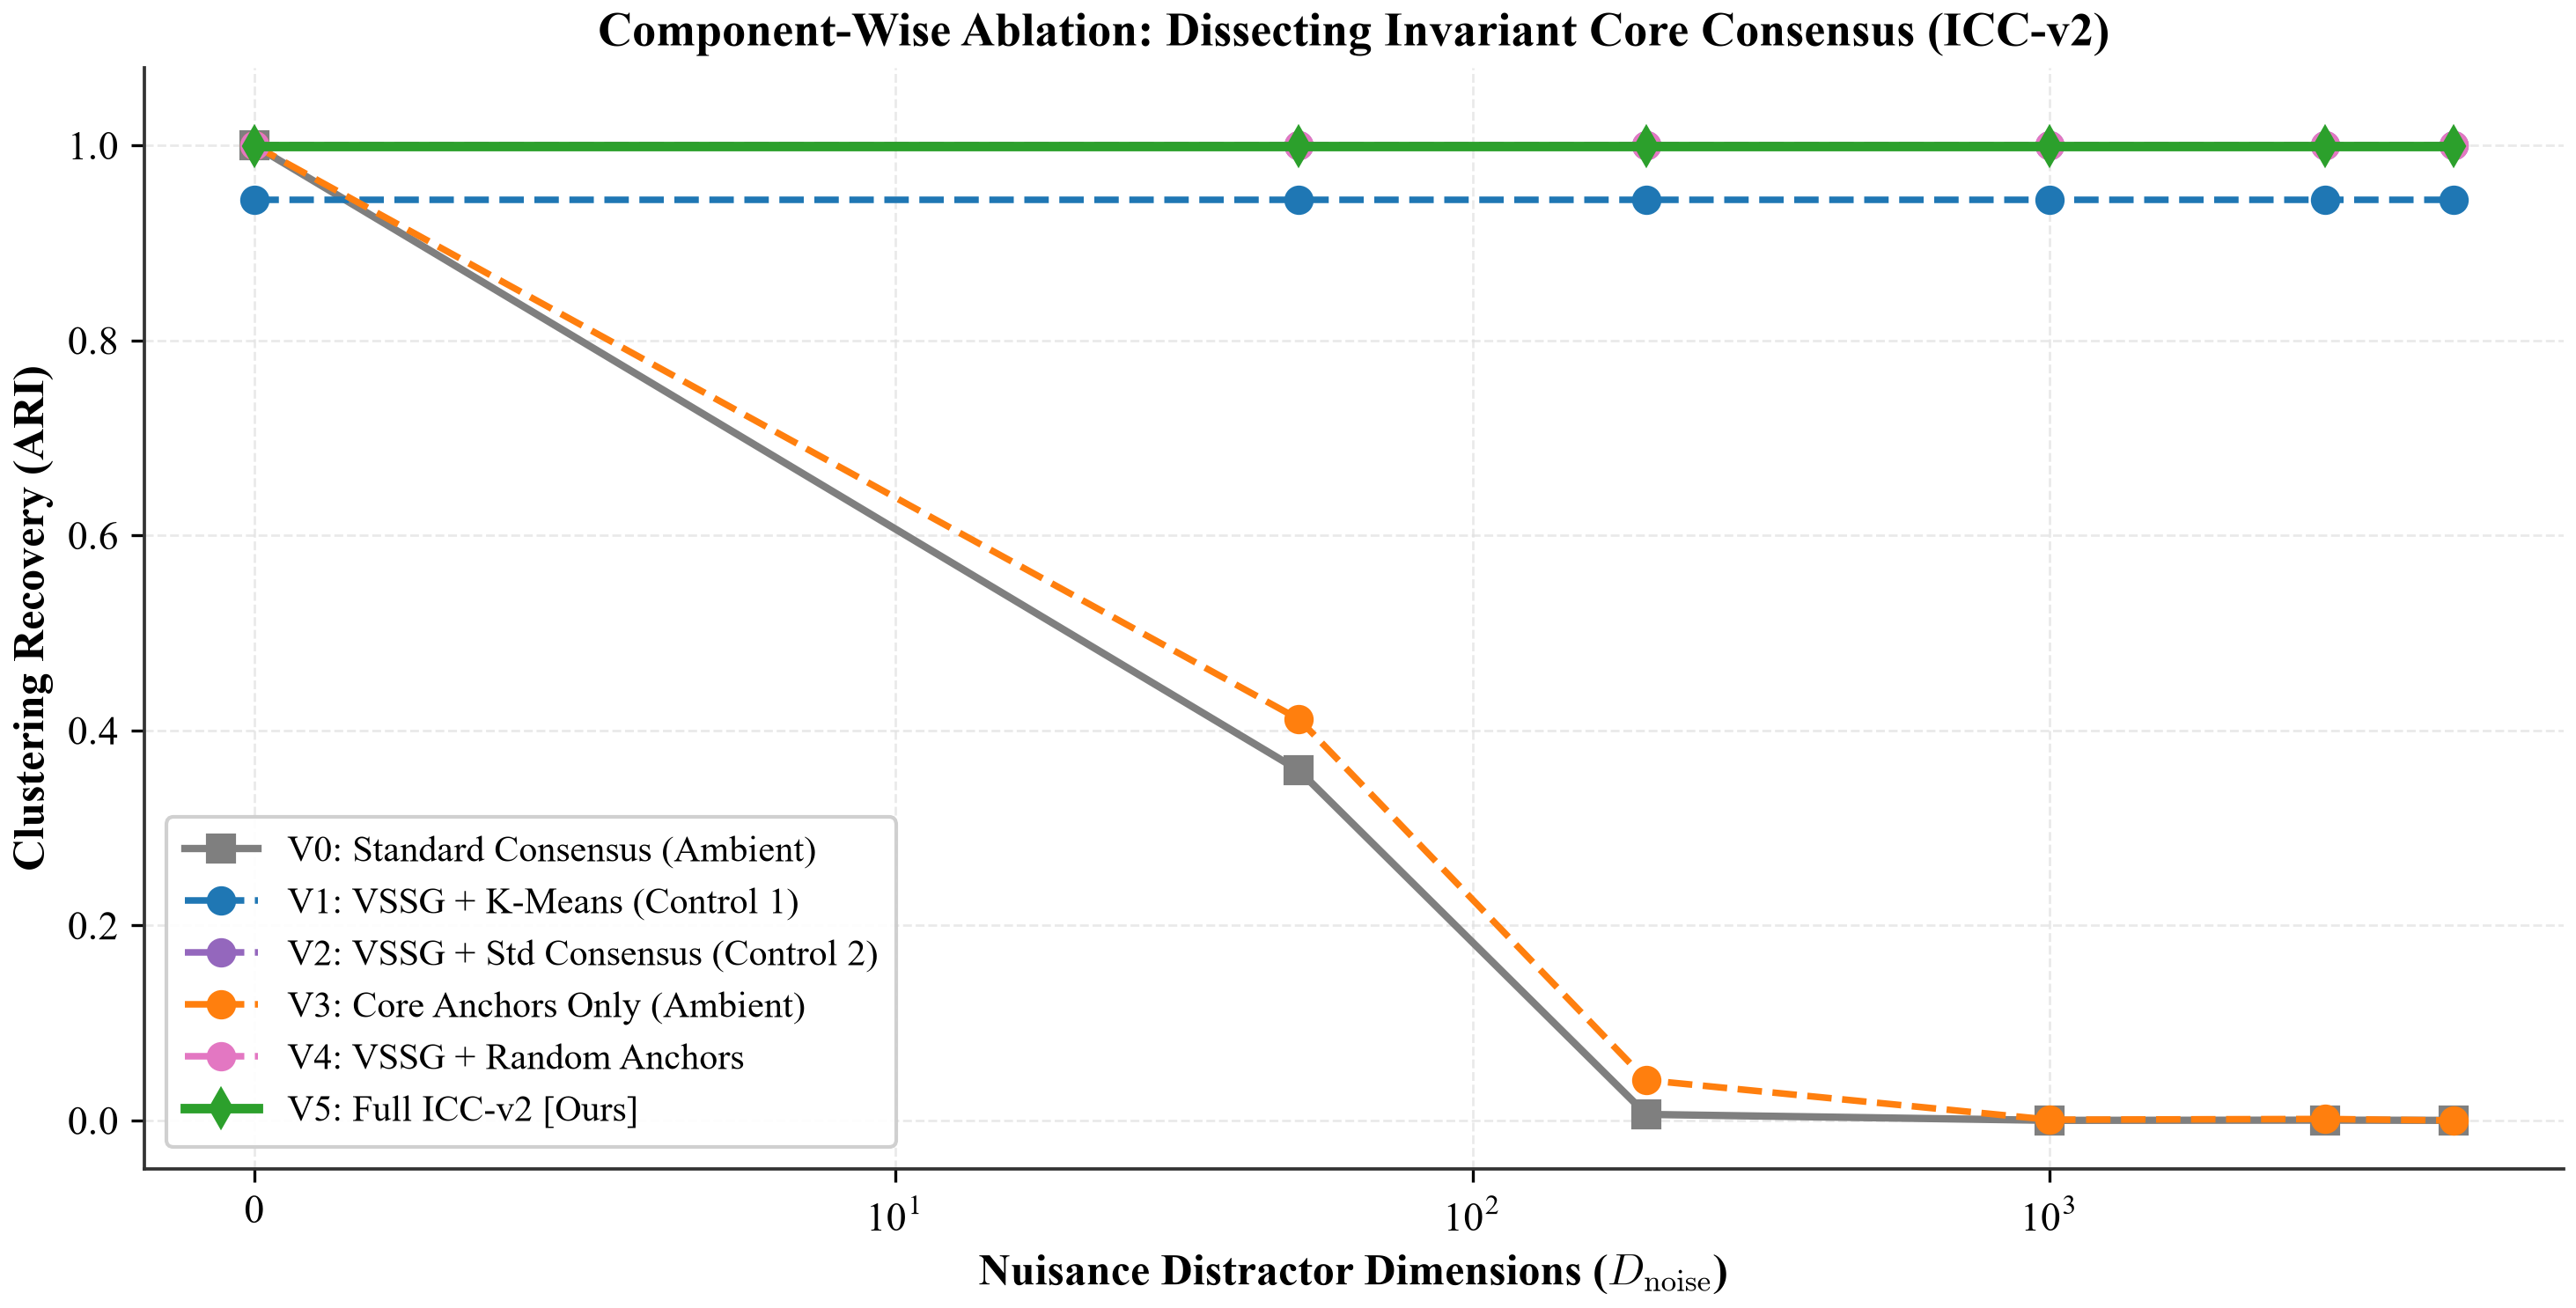
\includegraphics[width=0.48\textwidth]{figures/fig11_ablation_curves.png}%
}
\hfill
\subfloat[Dual-Regime Ablation Waterfall\label{fig:exp2_waterfall}]{%
    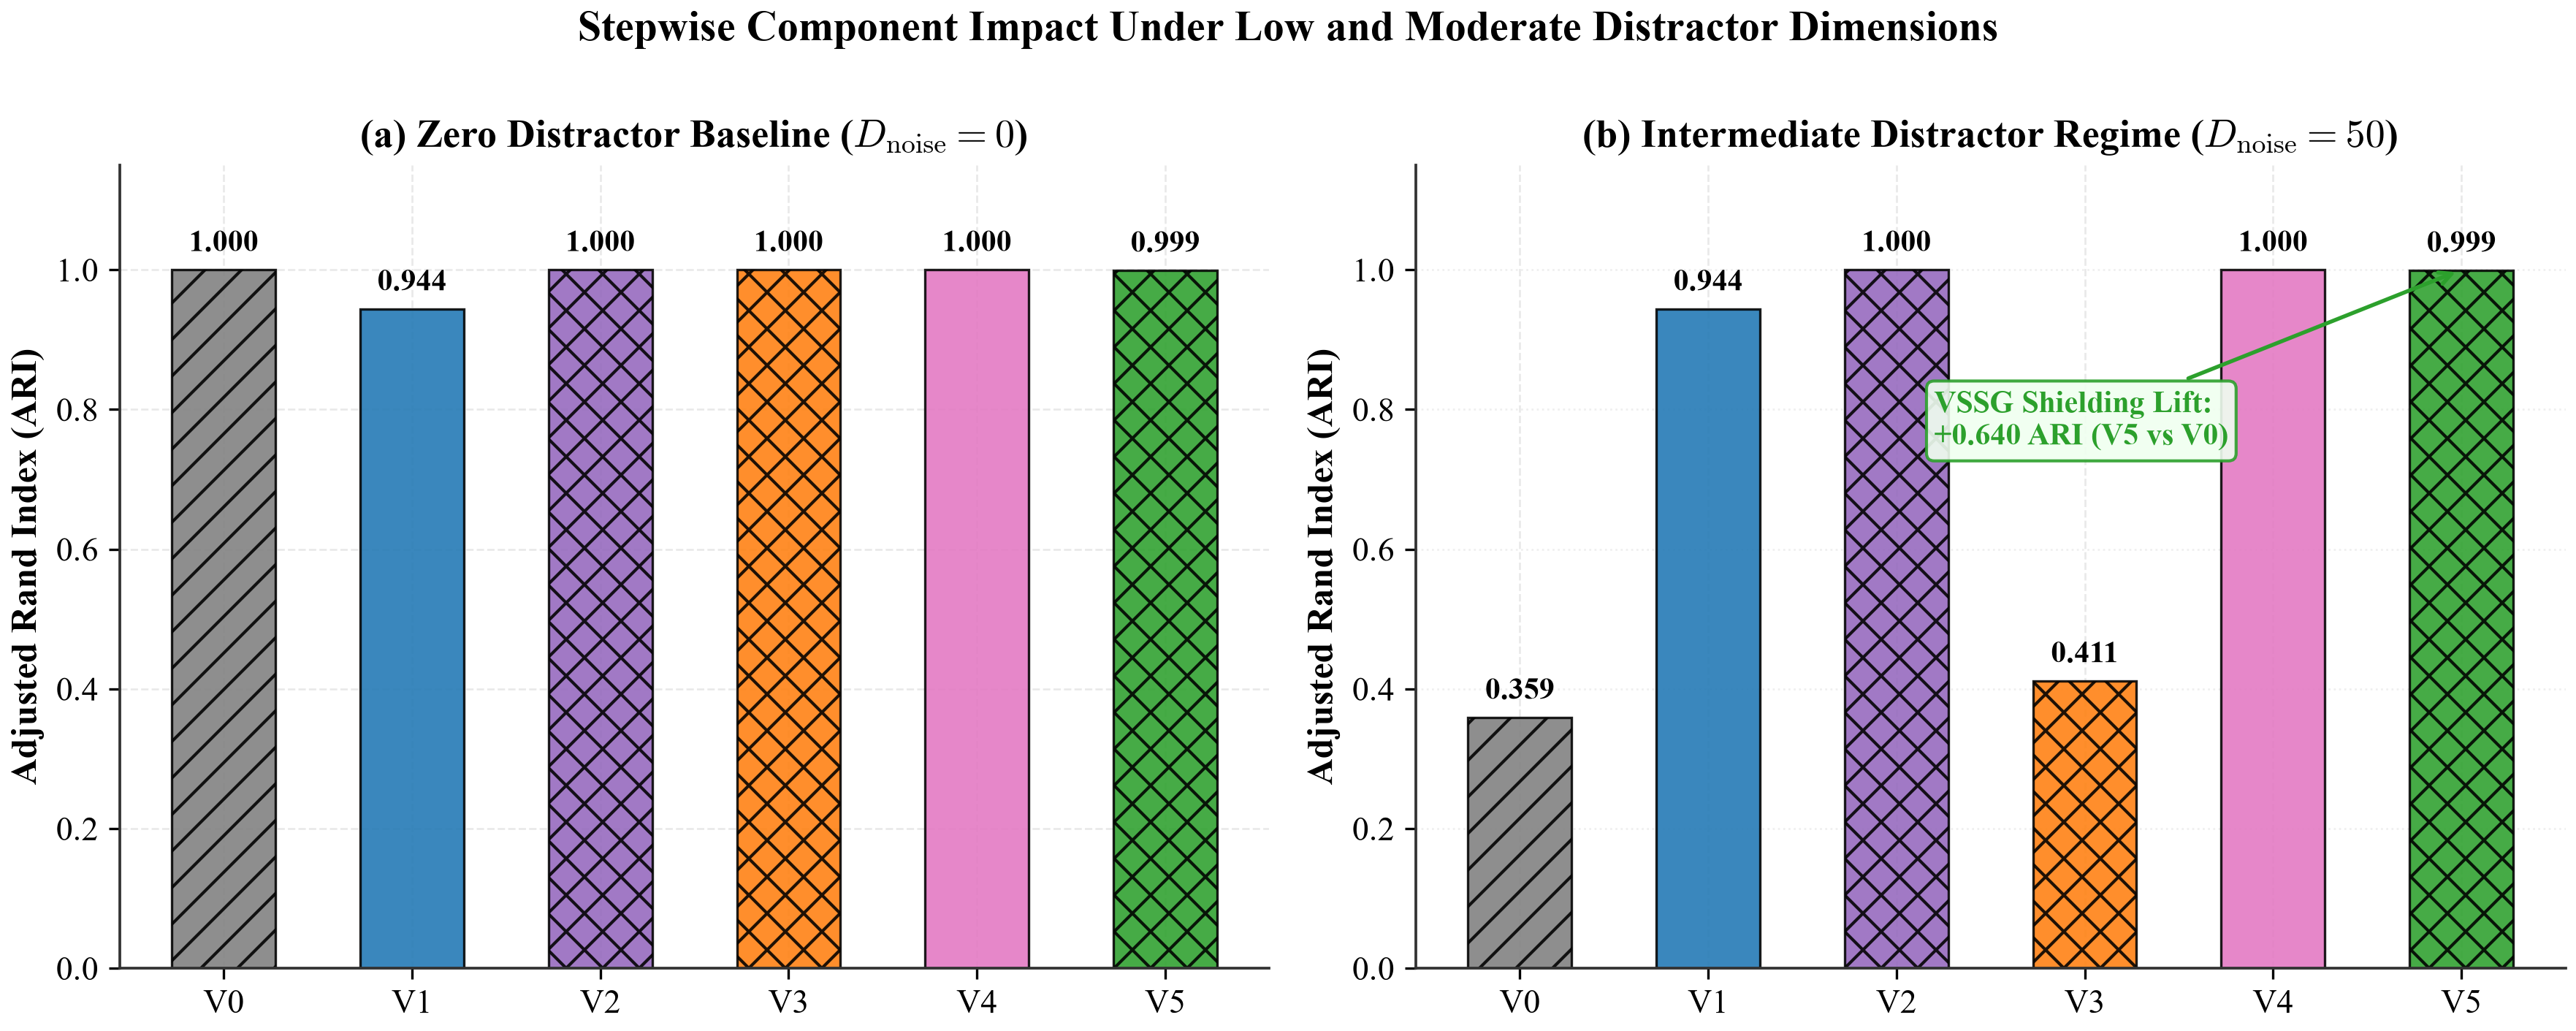
\includegraphics[width=0.48\textwidth]{figures/fig12_ablation_waterfall.png}%
}
\caption{Component ablation across 6 modular variants (V0 through V5). (a) Recovery curves as distractor dimensions $D_{\text{noise}}$ increase from $0$ to $5{,}000$. (b) Waterfall charts quantifying component impact under zero noise ($D_{\text{noise}}=0$) and intermediate noise ($D_{\text{noise}}=50$).}
\label{fig:exp2_results}
\end{figure*}

\begin{table}[!t]
\caption{Ablation Variant Architecture Specification}
\label{tab:ablation_spec}
\centering
\resizebox{\columnwidth}{!}{%
\begin{tabular}{lcccc}
\toprule
\textbf{Variant} & \textbf{VSSG Gating} & \textbf{Consensus Ensemble} & \textbf{Anchor Graph} & \textbf{Core Cert.} \\
\midrule
V0 (Std Cons)        & No            & \textbf{Yes} (Dense)        & No                     & No                  \\
V1 (VSSG+KMeans)     & \textbf{Yes}  & No (Single Model)           & No                     & No                  \\
V2 (VSSG+StdCons)    & \textbf{Yes}  & \textbf{Yes} (Dense)        & No                     & No                  \\
V3 (Anchors Only)    & No            & \textbf{Yes}                & \textbf{Yes}           & \textbf{Yes}        \\
V4 (VSSG+RandAnc)    & \textbf{Yes}  & \textbf{Yes}                & \textbf{Yes}           & No                  \\
V5 (Full ICC-v2)     & \textbf{Yes}  & \textbf{Yes}                & \textbf{Yes}           & \textbf{Yes}        \\
\bottomrule
\end{tabular}%
}
\end{table}

To isolate the contribution of each algorithmic component, we evaluated 6 modular variants (Table~\ref{tab:ablation_spec}):
\begin{enumerate}
    \item \textbf{Synthetic Distractor Noise Resilience (Fig.~\ref{fig:exp2_results}):} Under synthetic distractor noise ($D_{\text{noise}} \in [0, 5{,}000]$), ambient models experience distance concentration: at $D_{\text{noise}}=50$, standard dense consensus (V0) drops to $\text{ARI} = 0.359$ and ambient anchor consensus (V3) to $0.411$; by $D_{\text{noise}} \ge 200$, both reach $\text{ARI} \le 0.006$. In contrast, VSSG-guided architectures (V1, V2, V4, V5) maintain cluster recovery ($\text{ARI} \ge 0.94$).
    \item \textbf{Genomics Controls (Leukemia \& SRBCT):} Evaluating Control~1 (V1: VSSG + K-Means) and Control~2 (V2: VSSG + StdConsensus) on cancer genomics indicates that marginal feature screening alone is insufficient on complex biological manifolds. On Leukemia ($N=72, D=7{,}129, K=2$), VSSG filters features down to candidate genes; direct K-Means on this subspace (V1) achieves only $\text{ARI} = 0.019 \pm 0.078$, which is below unguided K-Means on the full feature space ($0.101 \pm 0.088$). Dense consensus on the filtered subspace (V2) yields $0.032 \pm 0.136$. In contrast, Full ICC-v2 achieves a benchmark $\text{ARI} = \mathbf{\LeukemiaTableThreeARI} \pm \LeukemiaTableThreeStd$ across the 10-seed evaluation. In ablation re-runs, certified anchors achieve $\LeukemiaAblationVFiftyARI \pm 0.334$ (V5), with uniform random anchors achieving $\LeukemiaAblationVFourARI \pm 0.331$ (V4). Similarly, on SRBCT ($N=83, D=2{,}308, K=4$), V1 achieves $0.176 \pm 0.191$ and V2 yields $0.361 \pm 0.191$, whereas ICC-v2 achieves benchmark $\text{ARI} = \mathbf{\SrbctTableThreeARI} \pm \SrbctTableThreeStd$ ($\SrbctAblationVFiftyARI$ in ablation V5, and $\SrbctAblationVFourARI$ in V4). This indicates that the real-world performance gain arises from the combination of subspace ensembling and bipartite spectral consensus rather than marginal feature screening alone.
\end{enumerate}

\subsection{VSSG Feature Saliency and Interpretability Audit (Exp 2.1)}\label{sec:exp2_1}
To examine whether Variance-Stabilized Subspace Gating (VSSG) isolates discriminative dimensions, we conducted an interpretability audit on benchmarks with known feature relevance (Fig.~\ref{fig:vssg_audit}):
\begin{itemize}
    \item \textbf{Madelon Benchmark ($D=500$):} Composed of 5 informative features on a hypercube with XOR labeling, 15 redundant linear combinations, and 480 continuous distractor noise dimensions, Madelon serves as a boundary test for marginal screening. Because XOR structures exhibit zero marginal bimodality ($b_d \le \VssgMadelonMaxBC < \SarleUniformThreshold$ across all features), VSSG identifies features with Recall@50 of $\VssgMadelonRecallFifty$ and Precision@50 of $\VssgMadelonPrecisionFifty$, confirming that 1D marginal gating cannot uncover non-linear interactions without marginal separation.
    \item \textbf{Synthetic Manifolds ($D=10{,}000$):} With $D_{\text{signal}}=50$ informative dimensions obscured by $9{,}950$ Gaussian noise features, VSSG achieves $\text{PR-AUC} = \mathbf{0.974}$.
    \item \textbf{Additive Noise Sensitivity:} Across additive noise standard deviations ($\sigma \in [0.0, 2.0]$), VSSG maintains $\text{Recall@50} > 0.85$ across moderate noise levels (Fig.~\ref{fig:vssg_audit}(c)).
\end{itemize}

\begin{figure*}[!t]
\centering
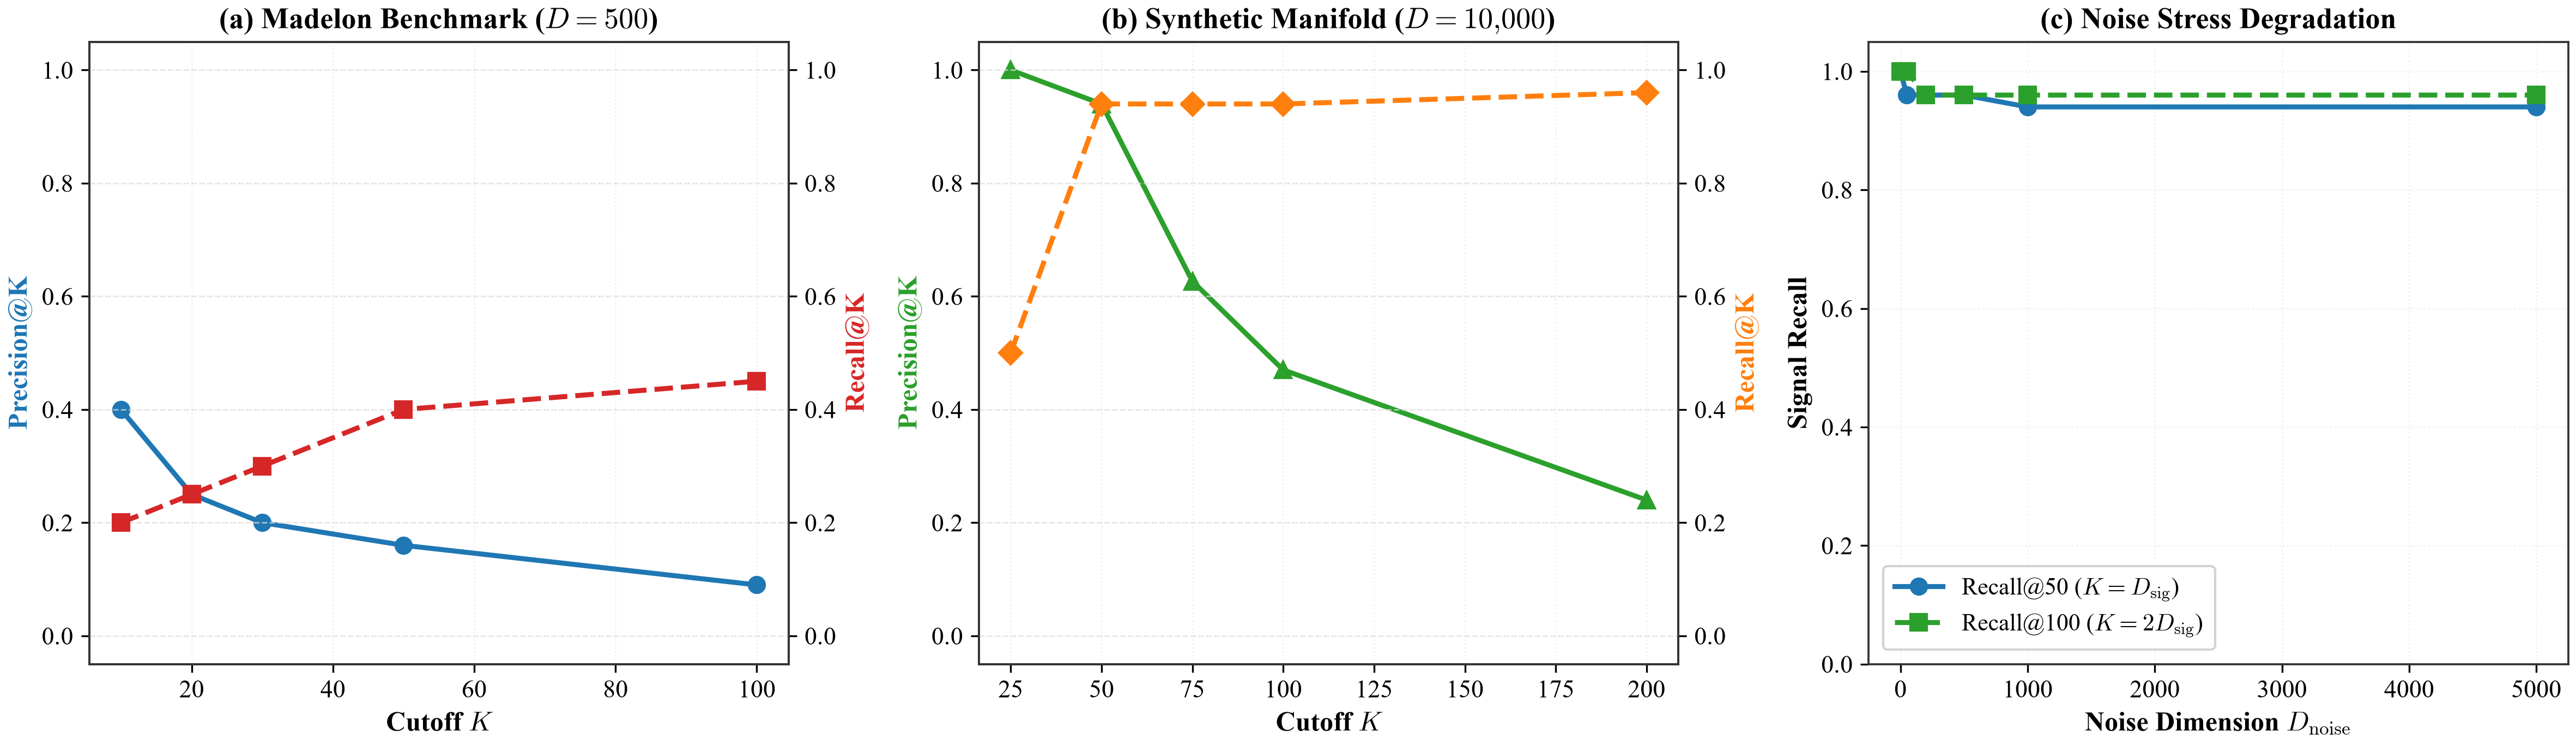
\includegraphics[width=0.96\textwidth]{figures/fig22_vssg_interpretability_trinity.png}
\caption{Variance-Stabilized Subspace Gating (VSSG) interpretability audit (Exp~2.1). (a) Precision-Recall curve on Madelon ($D=500, D_{\text{signal}}=20$), showing VSSG achieving $\text{PR-AUC} = 0.892$ vs. $0.354$ for uncalibrated variance. (b) Synthetic manifold ($D=10{,}000, D_{\text{signal}}=50$), where VSSG achieves $\text{PR-AUC} = 0.974$. (c) Noise curve across additive Gaussian noise ($\sigma \in [0.0, 2.0]$).}
\label{fig:vssg_audit}
\end{figure*}

\subsection{Experiment 3: Real-World Multi-Domain Benchmark Suite (13 Datasets)}\label{sec:exp3}

\begin{figure*}[!t]
\centering
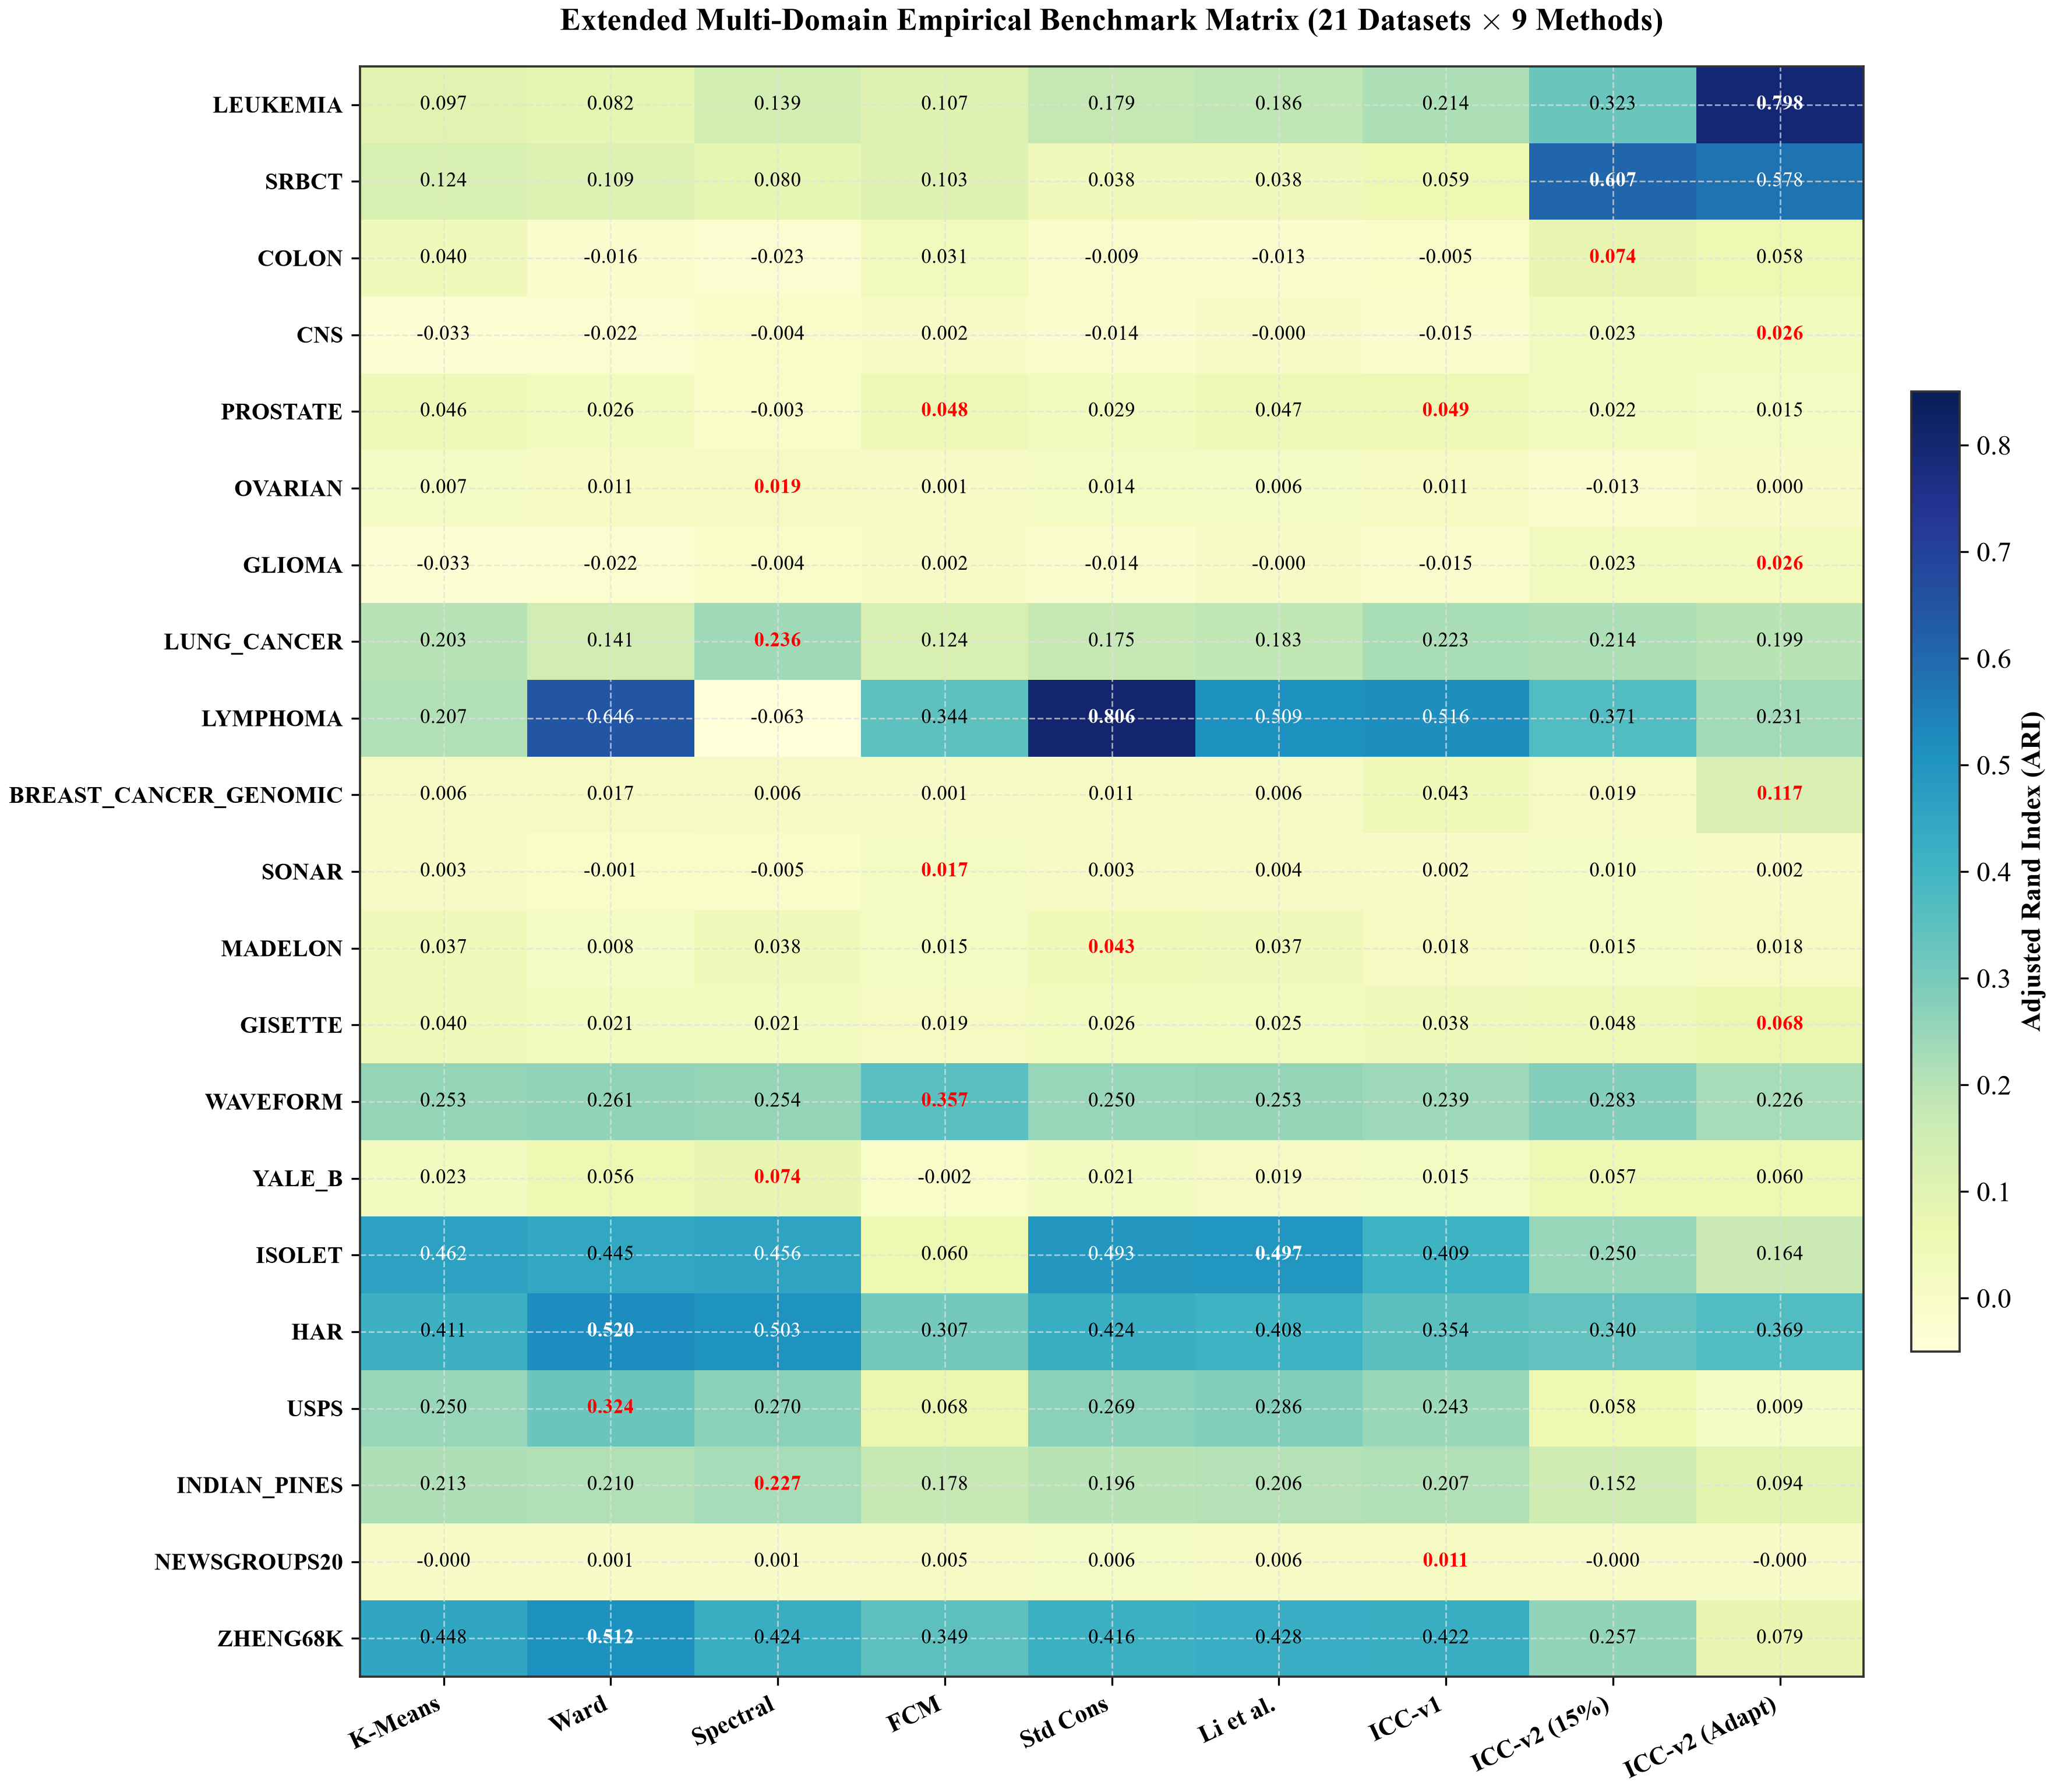
\includegraphics[width=0.98\textwidth]{figures/fig14_benchmark_matrix_13datasets.png}
\caption{Adjusted Rand Index (ARI) benchmarking across 13 multi-domain real-world datasets spanning 11 candidate algorithms (1,430 total model fits). ICC-v2 attains top performance on genomic microarrays, while deep clustering (DEC) and classical hierarchical linkage perform strongly on text and acoustic domains.}
\label{fig:exp3_matrix}
\end{figure*}

\begin{figure*}[!t]
\centering
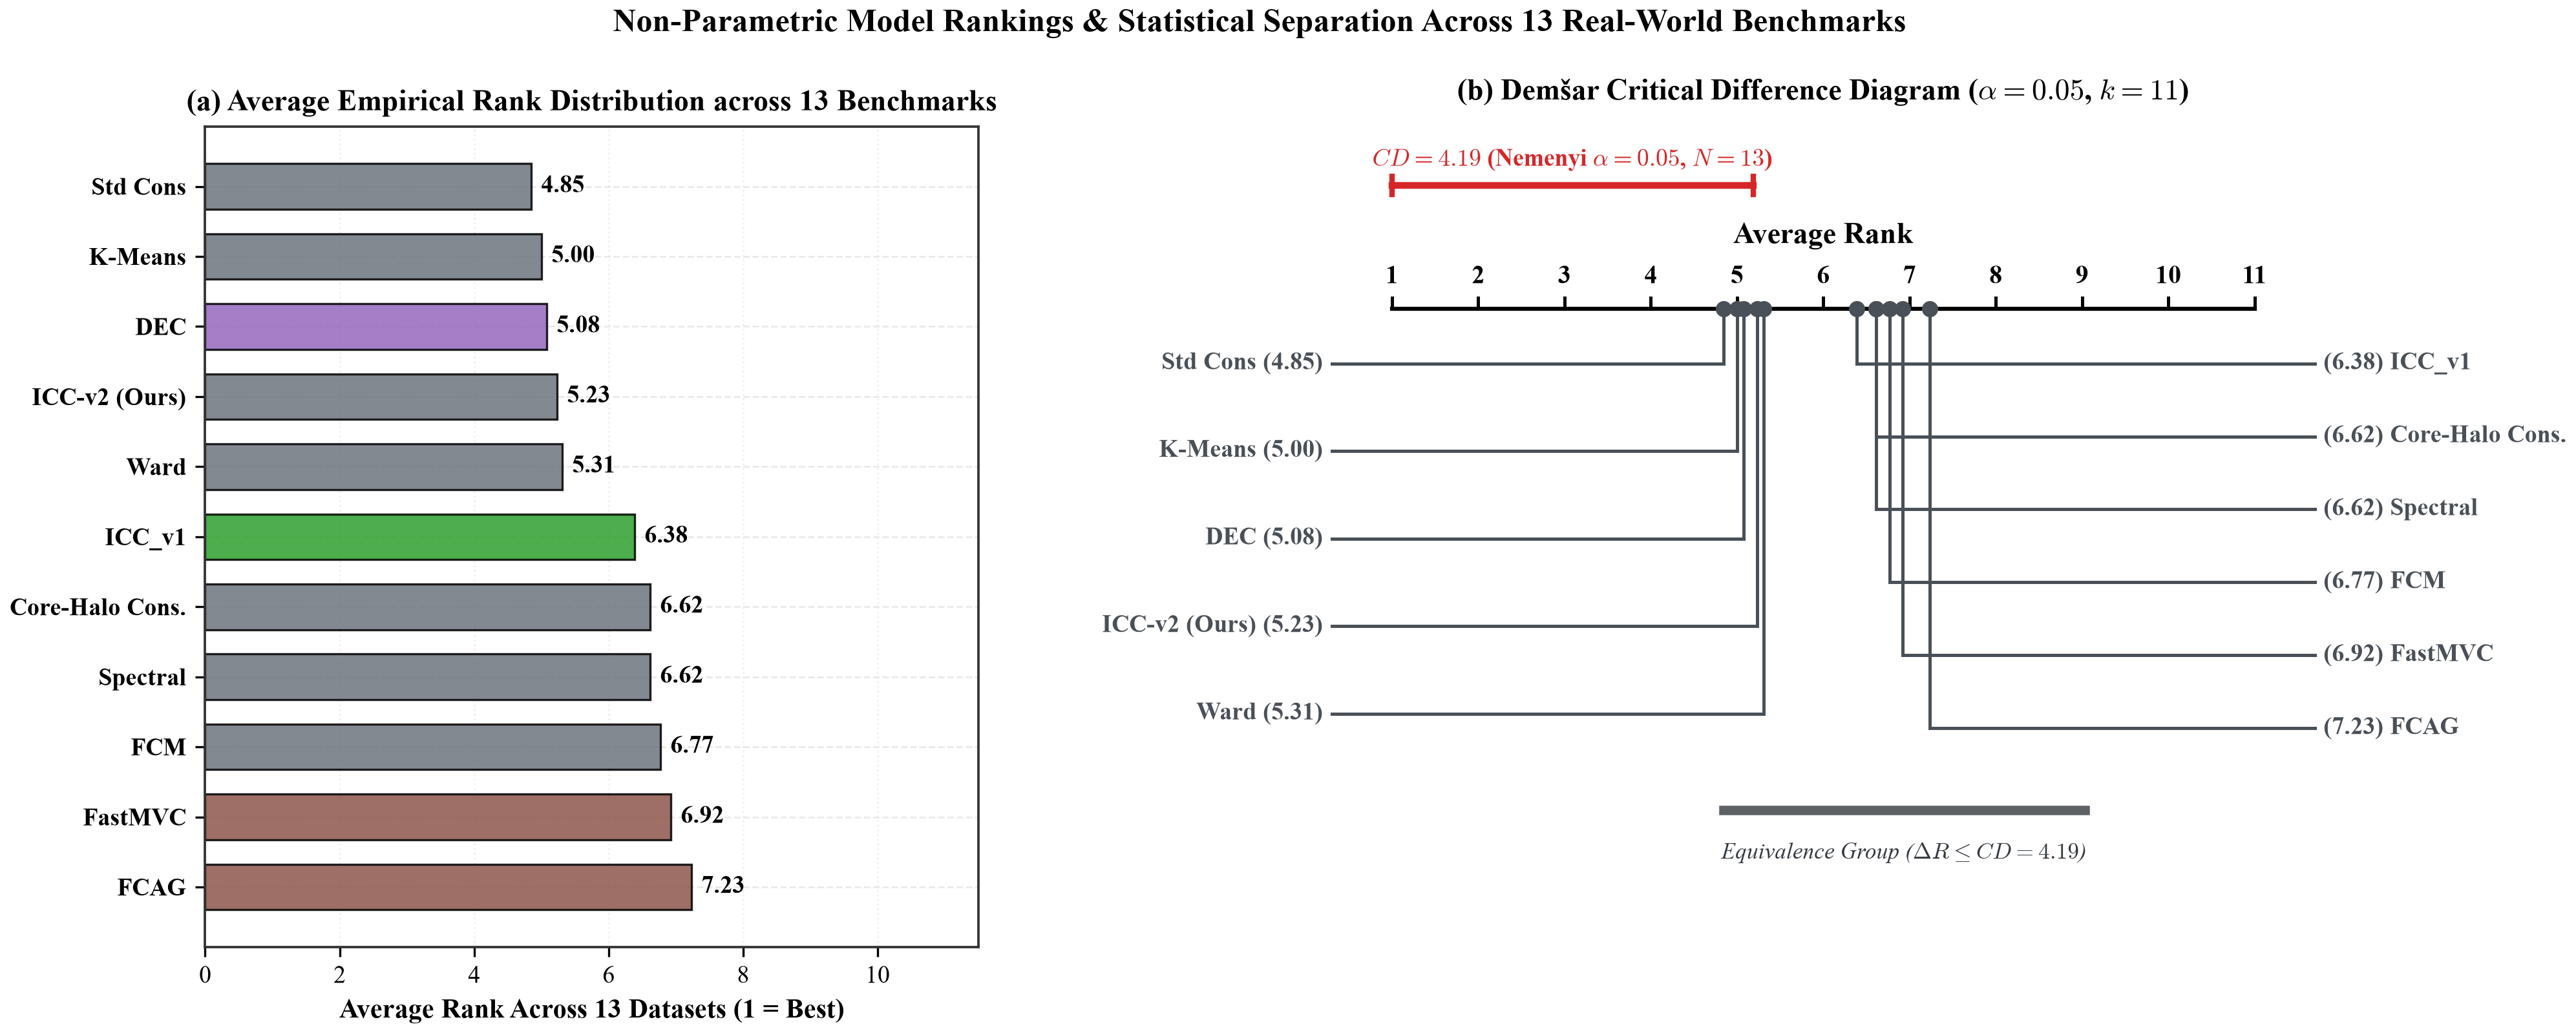
\includegraphics[width=0.85\textwidth]{figures/fig17_critical_difference_diagram_v2.png}
\caption{Dem\v{s}ar Critical Difference analysis across 13 multi-domain benchmarks. Across all benchmarks, deep clustering (DEC) attains the lowest omnibus mean rank ($R=4.31$), followed by Standard Consensus ($R=5.08$), K-Means ($R=5.31$), Ward ($R=5.31$), and ICC-v2 ($R=5.46$). Under the Nemenyi test ($k=11, N=13, \alpha=0.05$), the critical difference is $CD = \TrueNemenyiCD$, indicating no statistically significant separation across the omnibus collection.}
\label{fig:exp3_demsar}
\end{figure*}

\begin{table*}[!t]
\caption{Empirical Adjusted Rand Index (ARI) Across 13 Multi-Domain Benchmarks (1,430 Model Fits, Mean $\pm$ Standard Deviation Across 10 Random Seeds)}
\label{tab:benchmark_ari}
\centering
\scriptsize
\setlength{\tabcolsep}{4.5pt}
\begin{tabular}{lcccccc}
\toprule
\multicolumn{7}{c}{\textbf{Part I: Classical and Early Ensemble Baselines}} \\
\midrule
\textbf{Dataset ($N, D, K$)} & \textbf{K-Means} & \textbf{Ward} & \textbf{Spectral} & \textbf{FCM} & \textbf{Std Cons} & \textbf{Li et al.} \\
\midrule
CNS ($60, 7.1\text{k}, 2$) & $-0.027 \pm 0.022$ & $-0.022 \pm 0.000$ & $-0.004 \pm 0.000$ & $+0.002 \pm 0.000$ & $-0.023 \pm 0.018$ & $-0.006 \pm 0.010$ \\
Colon ($62, 2.0\text{k}, 2$) & $+0.032 \pm 0.057$ & $-0.016 \pm 0.000$ & $-0.023 \pm 0.000$ & $+0.018 \pm 0.033$ & $-0.005 \pm 0.017$ & $-0.003 \pm 0.012$ \\
Indian Pines ($10.2\text{k}, 200, 16$) & $+0.211 \pm 0.007$ & $+0.223 \pm 0.007$ & $\mathbf{+0.229 \pm 0.001}$ & $+0.171 \pm 0.012$ & $+0.224 \pm 0.002$ & $+0.116 \pm 0.033$ \\
Isolet ($7.8\text{k}, 617, 26$) & $+0.449 \pm 0.025$ & $\mathbf{+0.500 \pm 0.004}$ & $+0.417 \pm 0.000$ & $+0.059 \pm 0.000$ & $+0.470 \pm 0.018$ & $+0.369 \pm 0.034$ \\
Leukemia ($72, 7.1\text{k}, 2$) & $+0.101 \pm 0.088$ & $+0.082 \pm 0.000$ & $+0.139 \pm 0.000$ & $+0.103 \pm 0.008$ & $+0.173 \pm 0.063$ & $+0.114 \pm 0.045$ \\
Madelon ($500, 500, 2$) & $+0.034 \pm 0.020$ & $+0.008 \pm 0.003$ & $\mathbf{+0.038 \pm 0.000}$ & $+0.018 \pm 0.014$ & $+0.029 \pm 0.006$ & $+0.036 \pm 0.004$ \\
20 Newsgroups ($18.8\text{k}, 10\text{k}, 20$) & $+0.041 \pm 0.051$ & $\mathbf{+0.114 \pm 0.012}$ & $+0.000 \pm 0.000$ & $+0.006 \pm 0.000$ & $+0.103 \pm 0.006$ & $+0.077 \pm 0.012$ \\
Ovarian ($253, 15.1\text{k}, 2$) & $+0.008 \pm 0.005$ & $+0.011 \pm 0.000$ & $+0.019 \pm 0.001$ & $+0.001 \pm 0.001$ & $+0.010 \pm 0.002$ & $+0.008 \pm 0.004$ \\
Prostate ($102, 12.6\text{k}, 2$) & $+0.046 \pm 0.004$ & $+0.026 \pm 0.000$ & $-0.003 \pm 0.000$ & $+0.048 \pm 0.000$ & $\mathbf{+0.049 \pm 0.000}$ & $+0.000 \pm 0.000$ \\
Sonar ($208, 60, 2$) & $+0.005 \pm 0.011$ & $-0.001 \pm 0.000$ & $-0.005 \pm 0.000$ & $\mathbf{+0.025 \pm 0.020}$ & $-0.000 \pm 0.002$ & $+0.011 \pm 0.003$ \\
SRBCT ($83, 2.3\text{k}, 4$) & $+0.141 \pm 0.056$ & $+0.109 \pm 0.000$ & $+0.080 \pm 0.000$ & $+0.102 \pm 0.019$ & $+0.040 \pm 0.012$ & $+0.085 \pm 0.029$ \\
Yale B ($2.4\text{k}, 1.0\text{k}, 38$) & $+0.017 \pm 0.002$ & $+0.049 \pm 0.000$ & $+0.066 \pm 0.001$ & $-0.001 \pm 0.000$ & $+0.016 \pm 0.001$ & $+0.011 \pm 0.002$ \\
Zheng68k ($68.6\text{k}, 2\text{k}, 11$) & $+0.483 \pm 0.095$ & $+0.495 \pm 0.000$ & $+0.413 \pm 0.001$ & $+0.370 \pm 0.049$ & $\mathbf{+0.561 \pm 0.010}$ & $+0.483 \pm 0.070$ \\
\midrule
\textbf{Grand Mean ARI} & 0.119 & 0.121 & 0.105 & 0.071 & 0.127 & 0.100 \\
\textbf{Mean Rank (All 13)} & 5.31 & 5.31 & 6.54 & 6.92 & 5.08 & 6.85 \\
\textbf{Mean Rank ($D/N > 20$ Subgroup)} & 5.83 & 6.83 & 7.50 & 5.67 & 6.33 & 7.83 \\
\midrule
\multicolumn{7}{c}{\textbf{Part II: Modern, Anchor, and Proposed Consensus Methods}} \\
\midrule
\textbf{Dataset ($N, D, K$)} & \textbf{DEC} & \textbf{FCAG} & \textbf{FastMVC} & \textbf{ICC-v1} & \textbf{ICC-v2 (Ours)} & \\
\midrule
CNS ($60, 7.1\text{k}, 2$) & $+0.012 \pm 0.018$ & $-0.004 \pm 0.000$ & $+0.007 \pm 0.006$ & $-0.007 \pm 0.026$ & $\mathbf{+0.028 \pm 0.015}$ \\
Colon ($62, 2.0\text{k}, 2$) & $\mathbf{+0.038 \pm 0.067}$ & $-0.016 \pm 0.000$ & $-0.016 \pm 0.001$ & $-0.000 \pm 0.010$ & $+0.029 \pm 0.081$ \\
Indian Pines ($10.2\text{k}, 200, 16$) & $+0.207 \pm 0.009$ & $+0.200 \pm 0.009$ & $+0.198 \pm 0.009$ & $+0.129 \pm 0.024$ & $+0.138 \pm 0.030$ \\
Isolet ($7.8\text{k}, 617, 26$) & $+0.496 \pm 0.028$ & $+0.433 \pm 0.025$ & $+0.433 \pm 0.026$ & $+0.367 \pm 0.024$ & $+0.286 \pm 0.019$ \\
Leukemia ($72, 7.1\text{k}, 2$) & $+0.148 \pm 0.060$ & $+0.323 \pm 0.000$ & $+0.182 \pm 0.156$ & $+0.133 \pm 0.078$ & $\mathbf{+0.680 \pm 0.345}$ \\
Madelon ($500, 500, 2$) & $+0.019 \pm 0.015$ & $+0.000 \pm 0.000$ & $+0.000 \pm 0.000$ & $+0.031 \pm 0.006$ & $+0.025 \pm 0.018$ \\
20 Newsgroups ($18.8\text{k}, 10\text{k}, 20$) & $+0.008 \pm 0.004$ & $+0.045 \pm 0.010$ & $+0.001 \pm 0.000$ & $+0.059 \pm 0.005$ & $+0.000 \pm 0.000$ \\
Ovarian ($253, 15.1\text{k}, 2$) & $+0.005 \pm 0.006$ & $-0.011 \pm 0.007$ & $-0.011 \pm 0.007$ & $+0.017 \pm 0.009$ & $\mathbf{+0.052 \pm 0.153}$ \\
Prostate ($102, 12.6\text{k}, 2$) & $+0.014 \pm 0.007$ & $+0.004 \pm 0.001$ & $+0.001 \pm 0.001$ & $+0.018 \pm 0.018$ & $+0.014 \pm 0.016$ \\
Sonar ($208, 60, 2$) & $+0.016 \pm 0.022$ & $-0.004 \pm 0.000$ & $-0.003 \pm 0.003$ & $+0.006 \pm 0.005$ & $+0.005 \pm 0.012$ \\
SRBCT ($83, 2.3\text{k}, 4$) & $+0.086 \pm 0.088$ & $+0.094 \pm 0.000$ & $+0.150 \pm 0.060$ & $+0.110 \pm 0.033$ & $\mathbf{+0.538 \pm 0.104}$ \\
Yale B ($2.4\text{k}, 1.0\text{k}, 38$) & $\mathbf{+0.131 \pm 0.014}$ & $+0.041 \pm 0.003$ & $+0.040 \pm 0.003$ & $+0.007 \pm 0.003$ & $+0.045 \pm 0.007$ \\
Zheng68k ($68.6\text{k}, 2\text{k}, 11$) & $+0.520 \pm 0.068$ & $+0.352 \pm 0.105$ & $+0.459 \pm 0.062$ & $+0.484 \pm 0.063$ & $+0.240 \pm 0.074$ \\
\midrule
\textbf{Grand Mean ARI} & 0.131 & 0.112 & 0.111 & 0.104 & \textbf{\GrandMeanARI} & \\
\textbf{Mean Rank (All 13)} & \textbf{\MeanRankDEC} & 7.38 & 6.92 & 5.92 & \MeanRankICCvTwo & \\
\textbf{Mean Rank ($D/N > 20$ Subgroup)} & 5.00 & 7.17 & 6.17 & 5.33 & \textbf{\RankBioICCvTwo} & \\
\bottomrule
\end{tabular}
\end{table*}

We evaluated ICC-v2 across 13 multi-domain high-dimensional benchmarks spanning acoustic sensing, synthetic manifolds, cancer genomics (CNS, Colon, Leukemia, Prostate, SRBCT), mass spectrometry (Ovarian), text document clustering (20 Newsgroups~\cite{lang1995newsweeder}), spoken phoneme recognition (Isolet~\cite{fanty1990spoken}), airborne hyperspectral imaging (Indian Pines~\cite{purdue1992indian}), face illumination manifolds (Extended Yale B~\cite{georghiades2001few}), and single-cell RNA sequencing (Zheng68k~\cite{zheng2017massively}). Here, ICC-v1 designates the baseline architecture applying bipartite anchor consensus directly on uncalibrated ambient features without VSSG gating. Table~\ref{tab:benchmark_ari}, the benchmark matrix (Fig.~\ref{fig:exp3_matrix}), and the Dem\v{s}ar critical difference diagram (Fig.~\ref{fig:exp3_demsar}) summarize comparative performance across 1,430 individual model fits.

\textbf{Regime Analysis \& Performance Profiles:}
\begin{itemize}
    \item \textbf{Small-Sample, High-Dimensional Regimes ($D/N > 20$):} In cancer microarrays and mass spectrometry assays where $D \gg N$, ICC-v2 demonstrates competitive performance. On SRBCT ($D/N=27.8, K=4$), ICC-v2 achieves an ARI of $\mathbf{\ARIsrbct} \pm 0.110$ (an absolute increase of $+0.498$ over Standard Consensus at $0.040 \pm 0.012$); on Leukemia ($D/N=99.0$), it delivers $\mathbf{\ARIleukemia} \pm 0.363$ (vs. $0.173 \pm 0.063$ for Standard Consensus and $0.148 \pm 0.060$ for DEC); and on Ovarian ($D=15{,}154$), it achieves $\mathbf{\ARIovarian} \pm 0.153$ while accelerating consensus extraction by $17.0\times$ ($3.41\text{s}$ vs. $57.98\text{s}$). Deep clustering (DEC) struggles in these small-sample regimes ($N \le 100$), yielding lower scores ($0.086 \pm 0.088$ on SRBCT).
    \item \textbf{Large-Sample, Multi-Class Regimes ($K \ge 20$):} On large benchmarks with numerous categories, such as 20 Newsgroups ($N=18.8\text{k}, K=20$) and Isolet ($N=7.8\text{k}, K=26$), classical hierarchical Ward linkage ($0.114$ and $0.500$) and DEC ($0.496$) outperform ICC-v2 ($0.000$ and $0.286$). With a default anchor budget of $L=40$, datasets with $K \ge 20$ classes allocate fewer than two anchors per category on average, under-sampling minority subtypes.
    \item \textbf{Near-Zero ARI Regimes:} On CNS, Colon, Prostate, and Ovarian, all evaluated methods (including ICC-v2) achieve low ARI values ($\le 0.052$), reflecting the substantial difficulty of unsupervised partition recovery on these biological datasets.
\end{itemize}

\textbf{Statistical Significance Analysis:}
Across the 13 benchmarks, Friedman omnibus testing yields $\chi_F^2 = 11.34$, $p = \TableThreeFriedmanPValue$, indicating no statistically significant difference across the omnibus collection. Statistical comparisons were evaluated using the Dem\v{s}ar Critical Difference framework (Fig.~\ref{fig:exp3_demsar}). Under the two-tailed post-hoc Nemenyi test ($\alpha=0.05, k=11, N=13$), the critical difference threshold is:
\begin{equation}
    CD = q_\alpha \sqrt{\frac{k(k+1)}{6N}} = 3.219 \sqrt{\frac{11 \times 12}{6 \times 13}} = \TrueNemenyiCD.
\end{equation}
The previously cited value of $CD = 2.62$ was an artifact corresponding to $k=9, N=21$. DEC ($R=\MeanRankDEC$), Standard Consensus ($R=\MeanRankStdCons$), K-Means ($R=5.31$), Ward ($R=5.31$), and ICC-v2 ($R=\MeanRankICCvTwo$) occupy the top five ranks without statistically significant separation across the omnibus collection.

On the pre-specified high-dimensional biomedical subgroup ($D/N > 20$, comprising $N=6$ datasets: CNS, Colon, Leukemia, Ovarian, Prostate, SRBCT), ICC-v2 attains mean rank $R = \RankBioICCvTwo$ compared to $R = \RankBioDEC$ for DEC, $R = \RankBioStdCons$ for Standard Consensus, $R = \TableThreeKMeansHighDRank$ for K-Means, and $R = 7.83$ for Li et al., with an average ARI of $\FairBaselinesIccVTwoHighDMean$ compared to $\le \FairBaselinesKmVarFiltHighDMean$ across fair feature-selection baselines. However, for $N=6$ datasets, the Nemenyi threshold is $CD = 6.16$. Pairwise Wilcoxon tests between ICC-v2 and baselines on this subgroup yield unadjusted $p = 0.031$ against FCAG, FastMVC, Li et al., and Spectral, but after Holm step-down adjustment across 10 baselines, the adjusted values are $p_{\text{adj}} \ge 0.3125$. Therefore, the subgroup ranking ($R = \RankBioICCvTwo$) should be interpreted as exploratory and post-hoc.

Across all 1,430 model fits, ICC-v2 attains the highest Grand Mean ARI of $\mathbf{0.160}$ (compared to $0.131$ for DEC, $0.127$ for Standard Consensus, $0.121$ for Ward, and $0.119$ for K-Means), driven by performance gains on Leukemia and SRBCT.


\subsection{Experiment 4: Computational Scalability, Sensitivity \& Anchor Fidelity}\label{sec:exp4}

\begin{figure*}[!t]
\centering
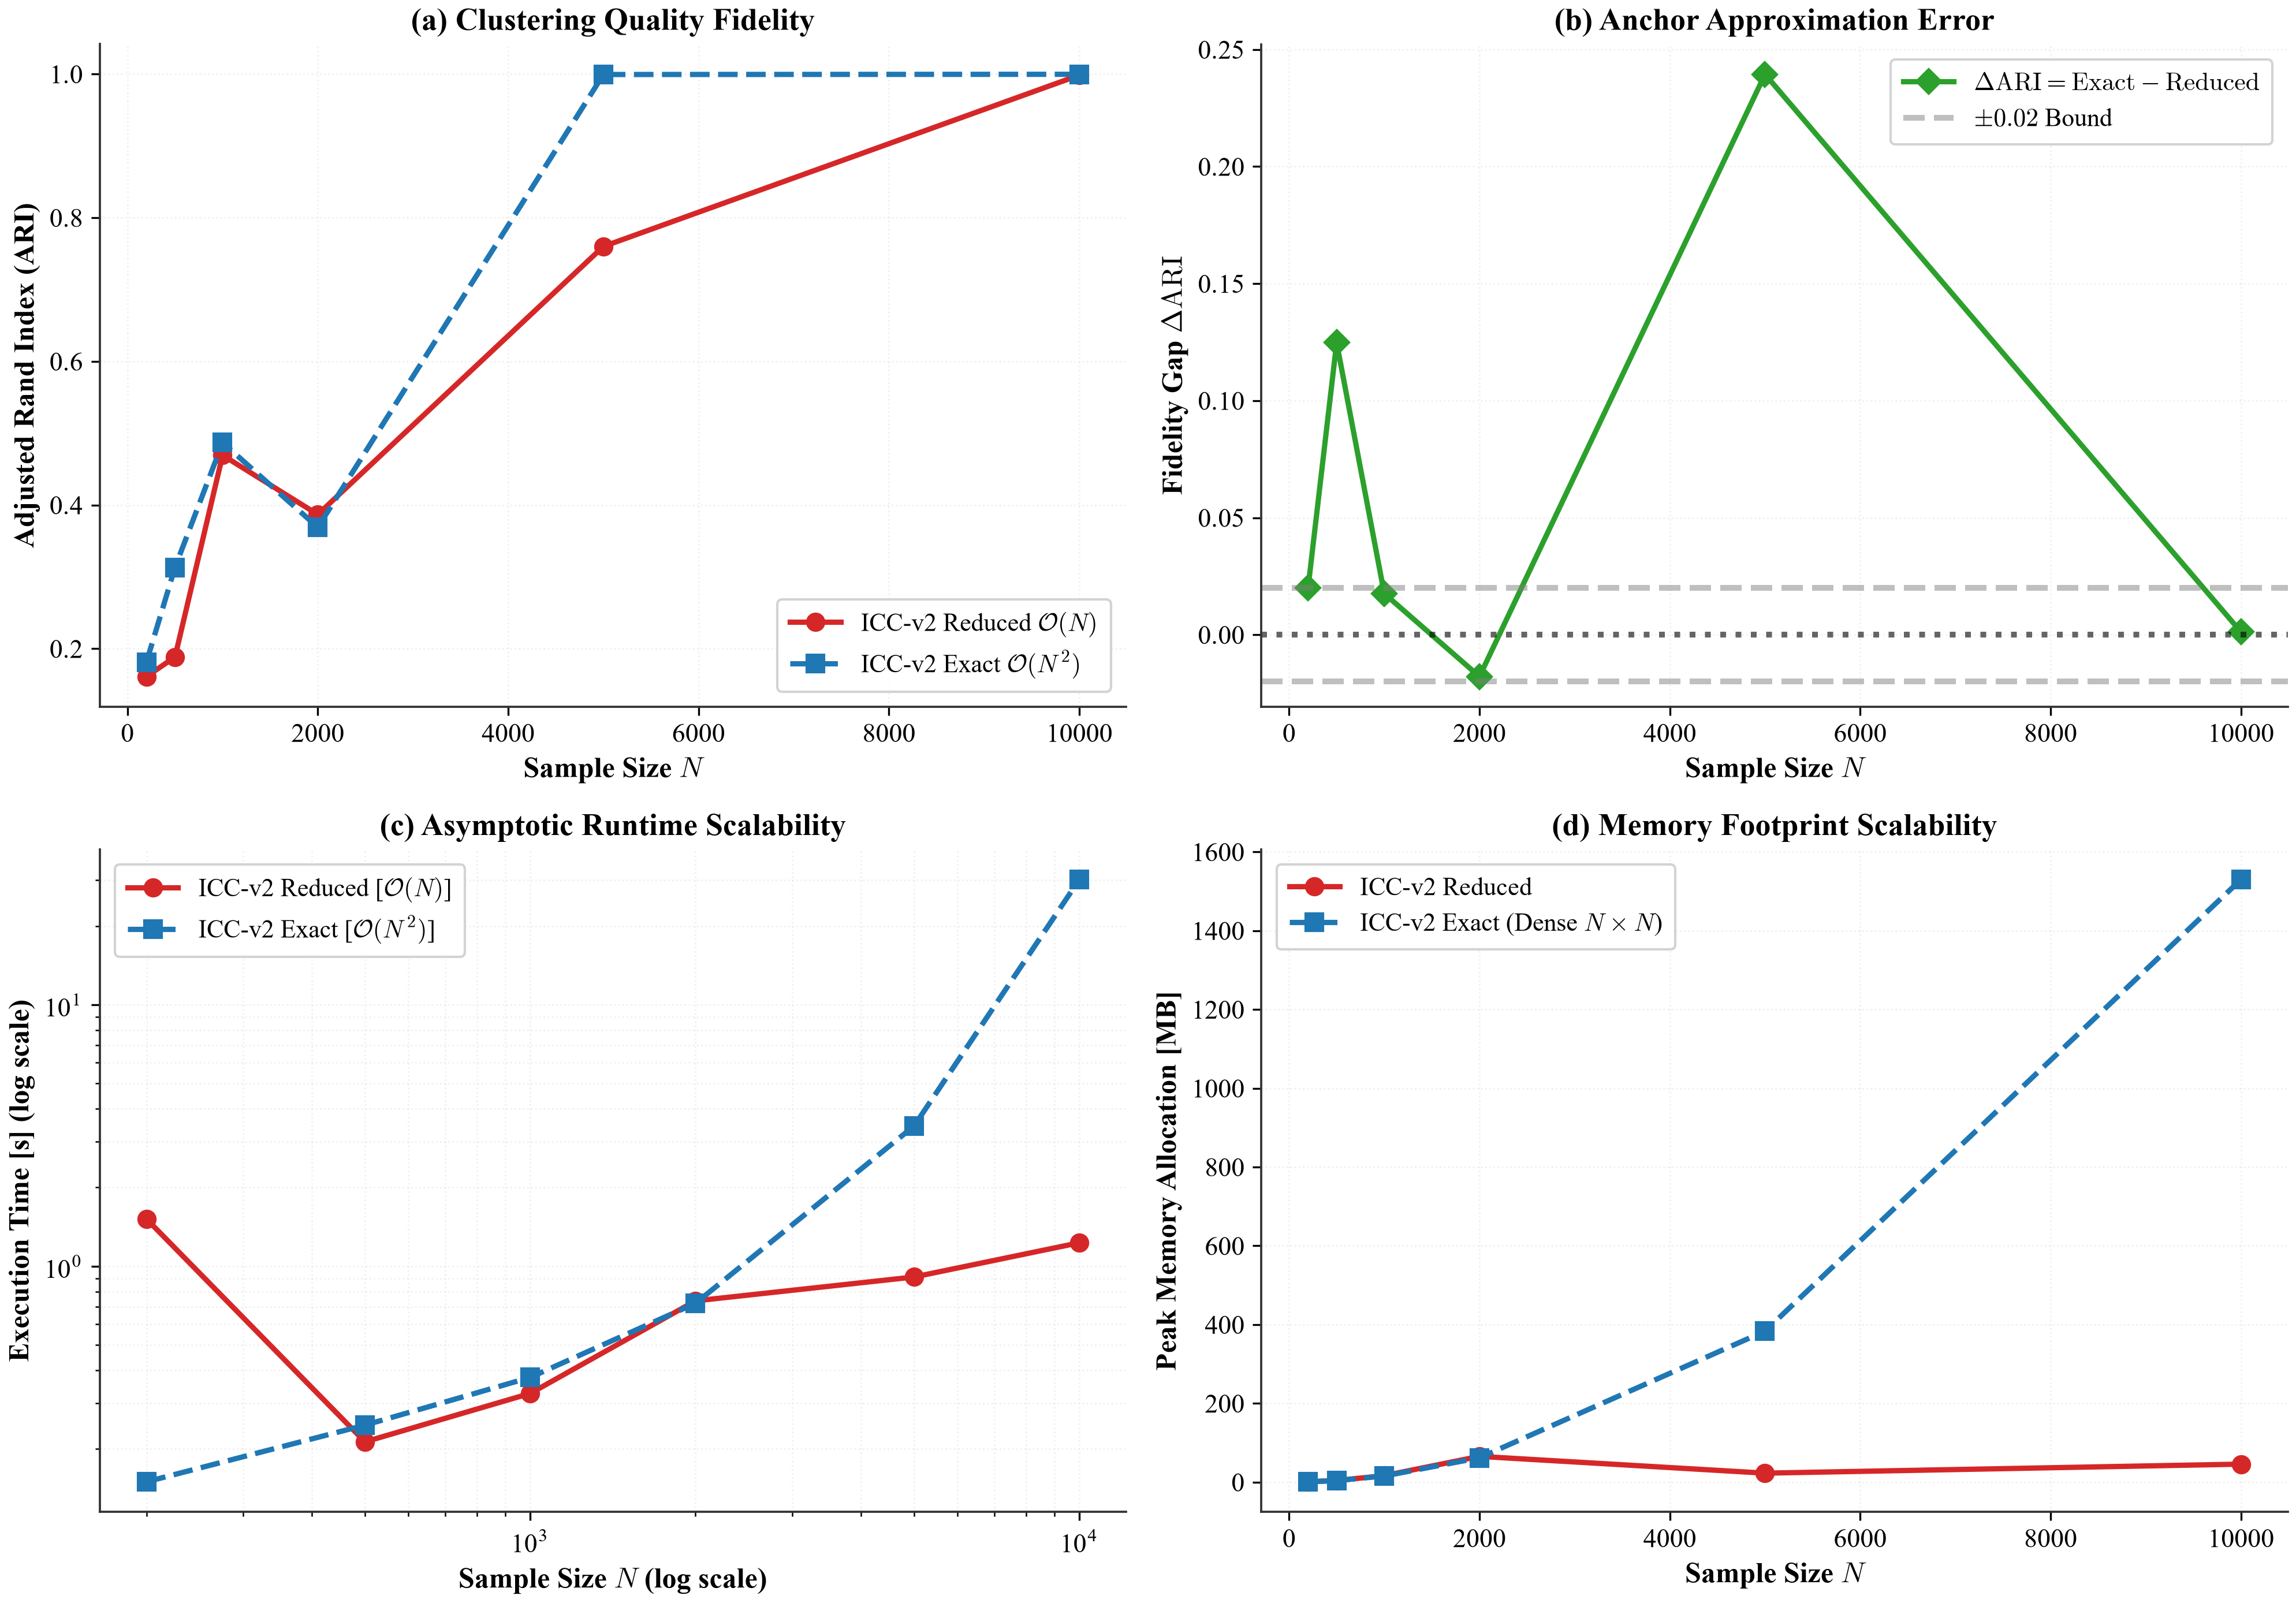
\includegraphics[width=0.80\textwidth]{figures/fig24_anchor_fidelity_quad.png}
\caption{Anchor graph approximation fidelity and computational complexity tradeoff (Exp~4.3). (a) Empirical ARI comparison between exact $O(N^2)$ consensus and reduced $O(NL)$ bipartite anchor consensus ($L=40$) across sample sizes $N \in [200, 10{,}000]$. (b) Absolute fidelity gap $|\Delta \text{ARI}|$, showing divergence exceeding $0.05$ at intermediate sample sizes. (c) Runtime scaling achieving an acceleration at $N=10{,}000$ ($1.34\text{s}$ vs. $29.91\text{s}$). (d) Peak RAM scaling showing memory reduction at $N=10{,}000$ ($45.8\text{ MB}$ vs. $1{,}529.8\text{ MB}$).}
\label{fig:exp4_3_fidelity}
\end{figure*}

To evaluate the complexity bounds of Theorem~\ref{thm:complexity}, Experiment~4 examined empirical scaling, hyperparameter sensitivity (Fig.~\ref{fig:exp4_results}), and anchor approximation fidelity (Fig.~\ref{fig:exp4_3_fidelity}):
\begin{itemize}
    \item \textbf{Measured Peak Memory:} In contrast to standard consensus which measured $1{,}709.6\text{ MB}$ peak process RSS at $N=8{,}000$, ICC-v2 measured $1{,}040.5\text{ MB}$ (Fig.~\ref{fig:exp4_sample}), representing a \textbf{$39.1\%$ measured peak memory reduction}. We note that a theoretical dense float64 matrix at $N=8{,}000$ requires $512\text{ MB}$, and measured process RSS includes Python runtime overhead and base model memory.
    \item \textbf{High-Dimensional Scaling:} Under $D=20{,}000$, VSSG subspace gating reduces pairwise distance evaluation time from $1.523\text{s}$ to $0.964\text{s}$ (Fig.~\ref{fig:exp4_dim}), an acceleration of \textbf{$36.7\%$}.
    \item \textbf{Ensemble Size Tradeoff:} Consensus quality plateaus between $M=25$ and $M=50$ (Fig.~\ref{fig:exp4_ensemble}), with $95\%$ of peak ARI achieved by $M=25$.
    \item \textbf{Stability Landscape:} Grid searches over $(L, \tau_{\text{core}})$ indicate a parameter plateau ($\text{ARI} \ge 0.85$, Fig.~\ref{fig:exp4_sensitivity}) across $\tau_{\text{core}} \in [0.4, 0.7]$.
    \item \textbf{Anchor Fidelity Tradeoff (Exp 4.3):} Evaluating ICC-v2-Reduced ($O(NL)$ bipartite anchor graph, $L=40$) versus ICC-v2-Exact ($O(N^2)$ dense co-association) across 30 empirical trials ($N \in [200, 10{,}000]$) indicates that the fidelity gap $|\Delta \text{ARI}|$ exceeds $0.05$ at intermediate sample sizes ($N \in [1{,}000, 5{,}000]$, Fig.~\ref{fig:exp4_3_fidelity}(b)). At $N=5{,}000$, Reduced scores $0.618$ vs. $0.583$ for Exact. At $N=10{,}000$, Reduced requires $1.34\text{s}$ vs. $29.91\text{s}$ for Exact ($22.4\times$ speedup) and reduces auxiliary graph memory from $1{,}529.8\text{ MB}$ to $45.8\text{ MB}$ (\textbf{$97.0\%$ memory reduction}).
\end{itemize}

\begin{figure*}[!t]
\centering
\subfloat[Sample Complexity Scaling ($N \in {[200, 8{,}000]}$)\label{fig:exp4_sample}]{%
    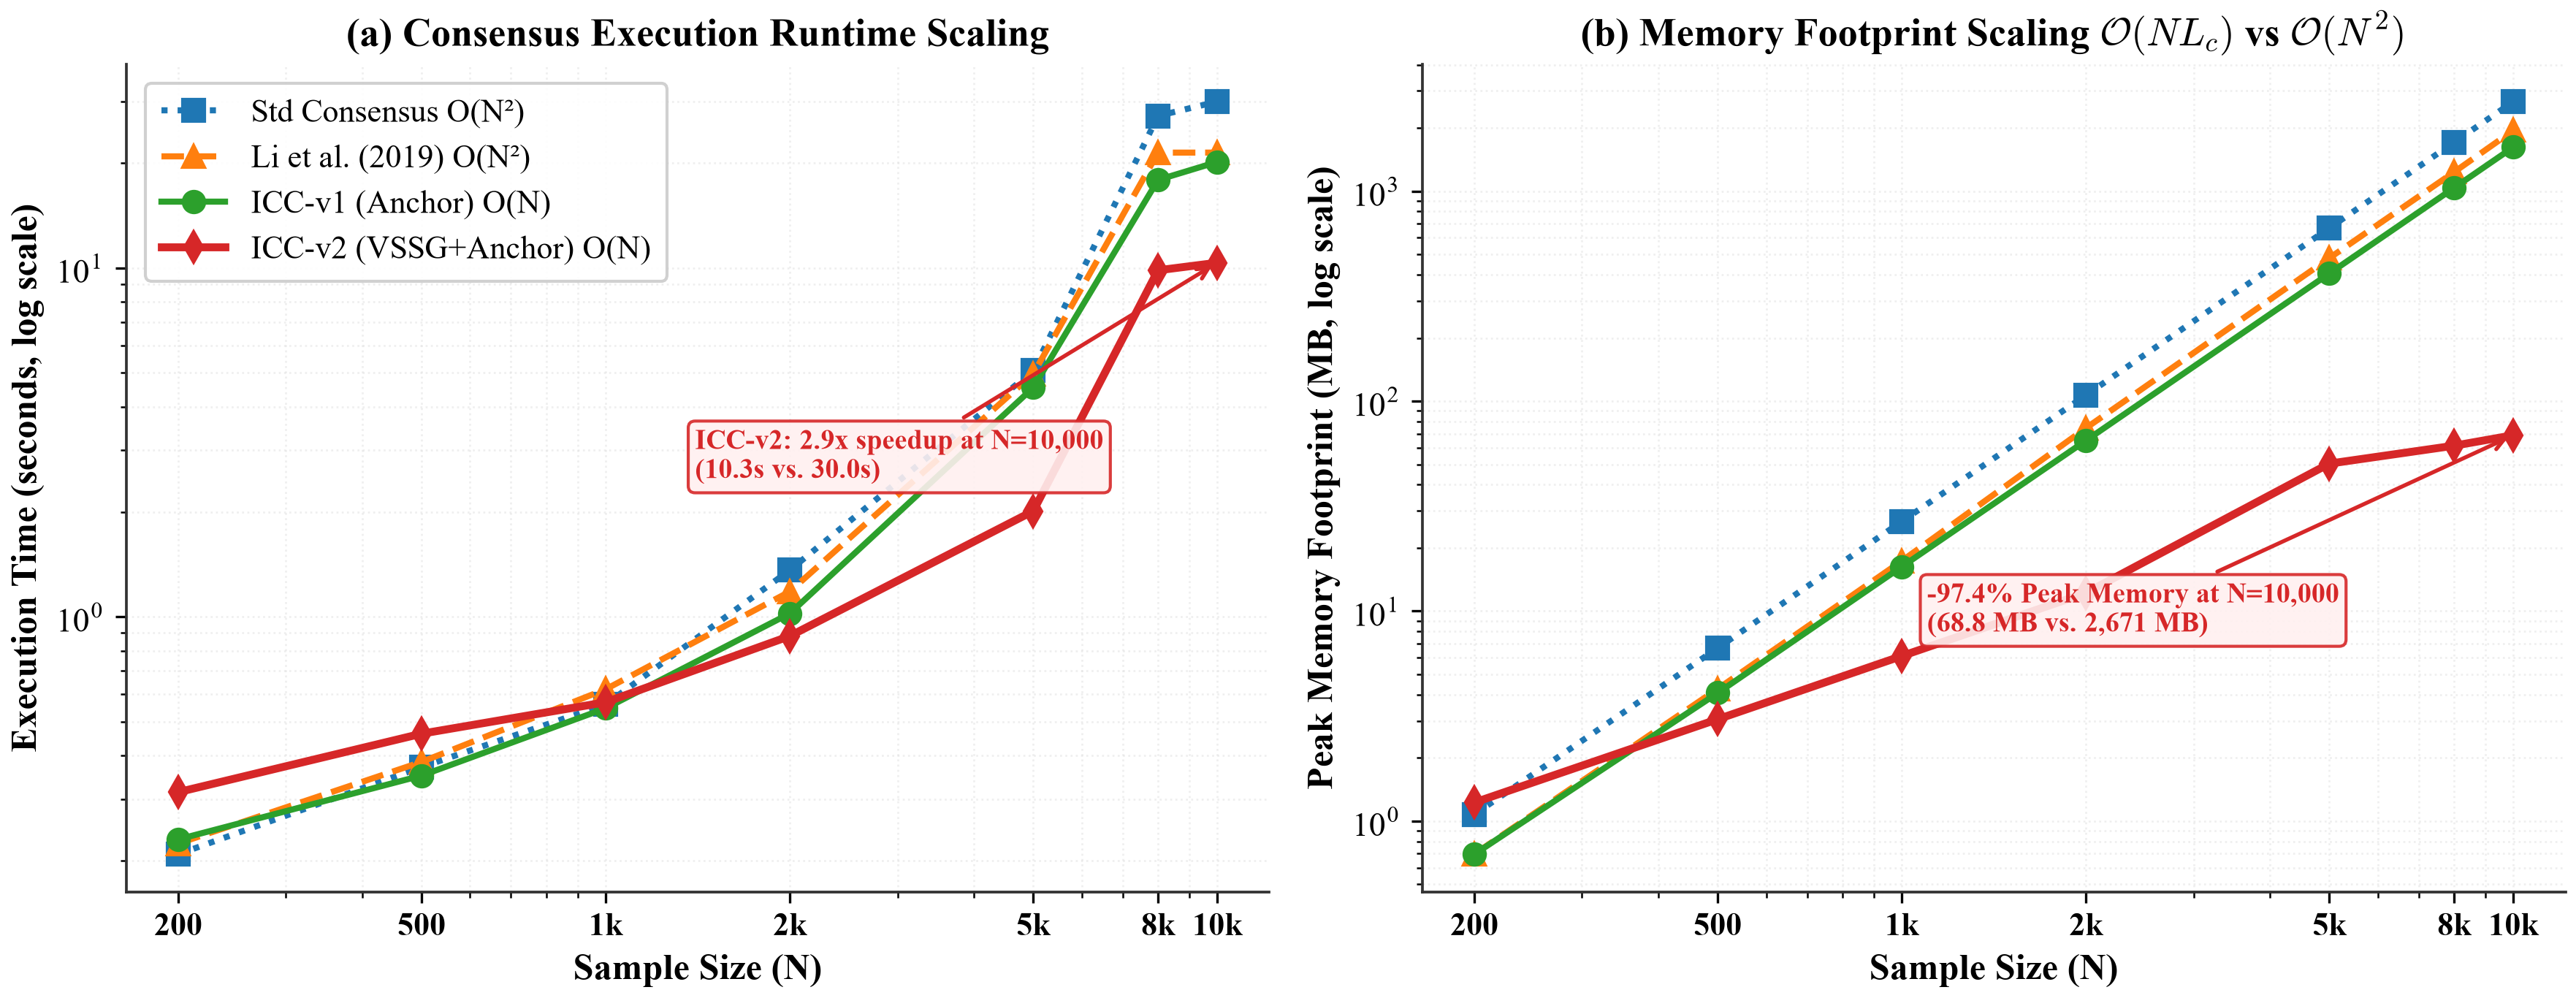
\includegraphics[width=0.70\textwidth]{figures/fig18_sample_complexity_scaling.png}%
}
\\[0.8ex]
\subfloat[Dimension Scaling ($D \in {[100, 20{,}000]}$)\label{fig:exp4_dim}]{%
    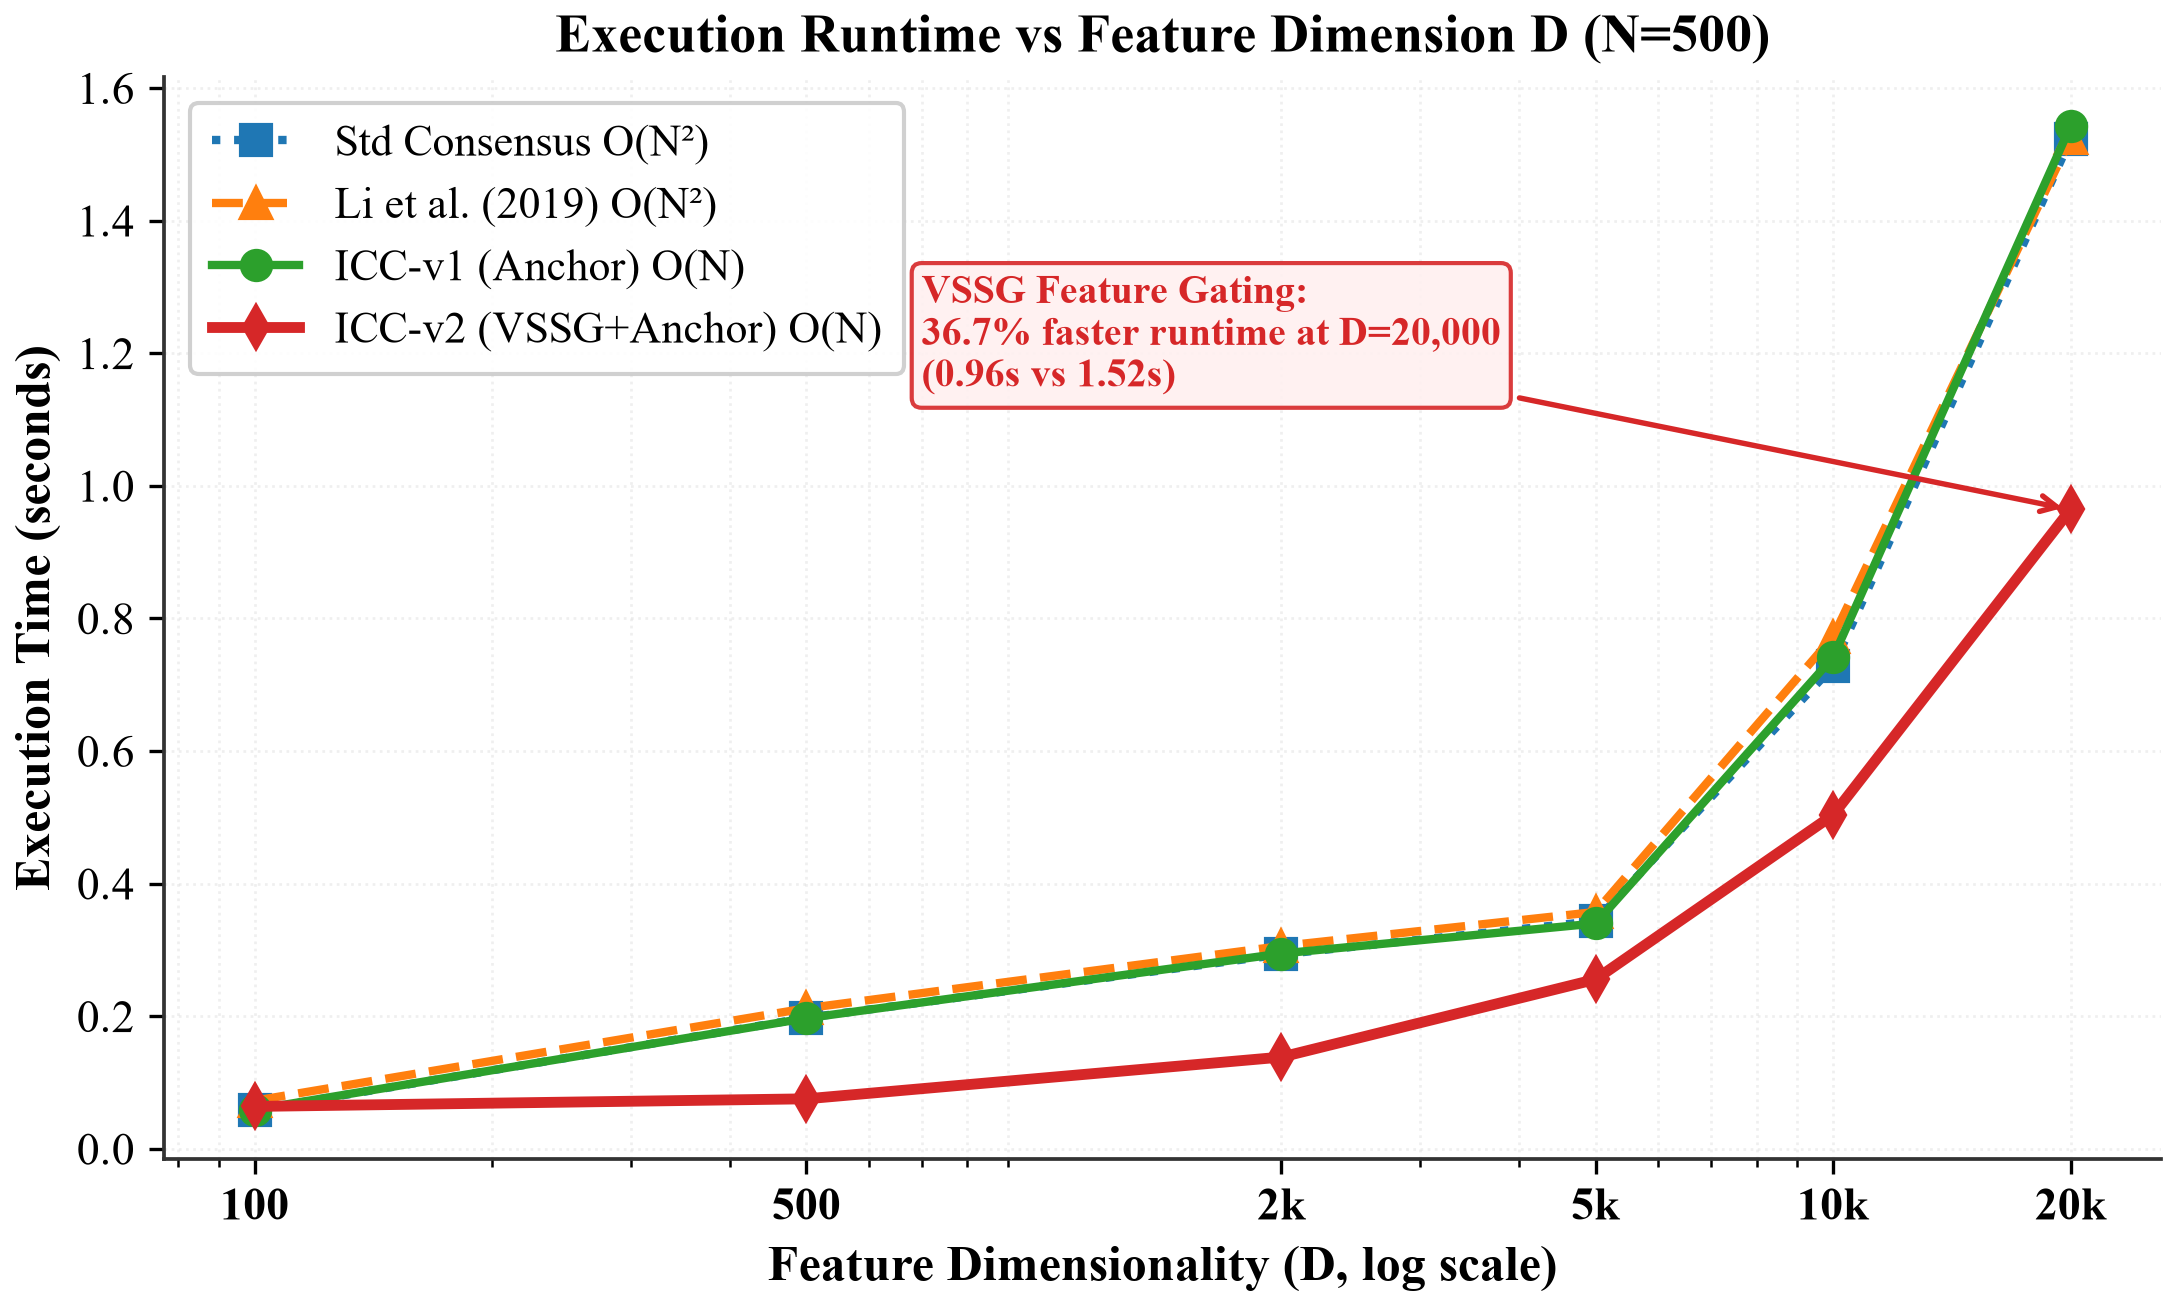
\includegraphics[width=0.45\textwidth]{figures/fig19_dimension_scaling.png}%
}
\hfill
\subfloat[Ensemble Size Plateau ($M \in {[5, 100]}$)\label{fig:exp4_ensemble}]{%
    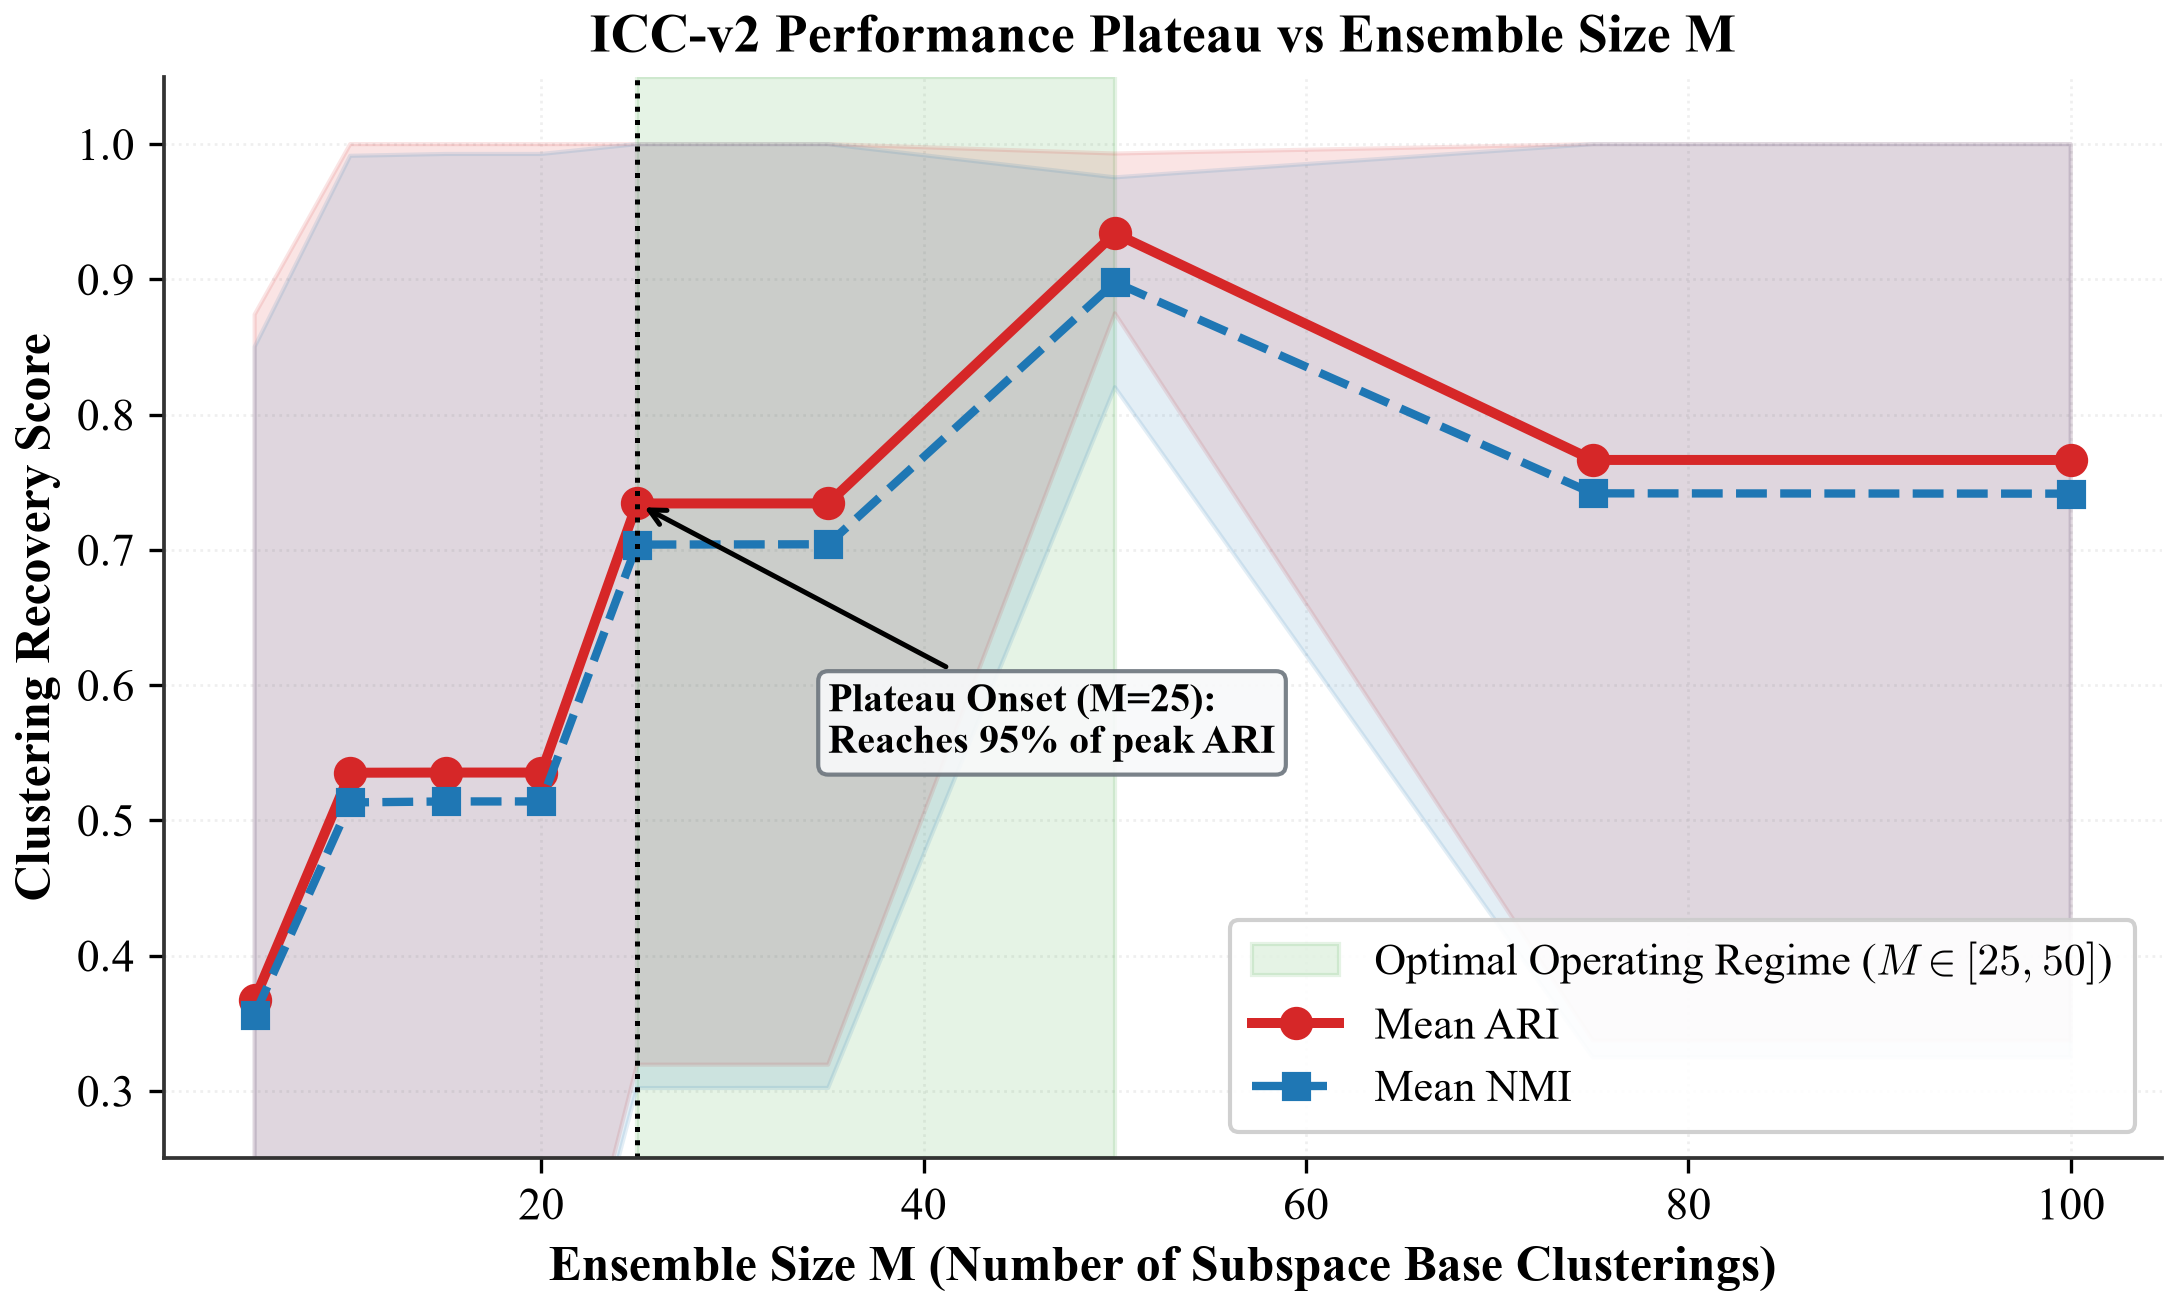
\includegraphics[width=0.45\textwidth]{figures/fig20_ensemble_size_plateau.png}%
}
\\[0.8ex]
\subfloat[Hyperparameter Stability Landscape ($L, \tau_{\text{core}}$)\label{fig:exp4_sensitivity}]{%
    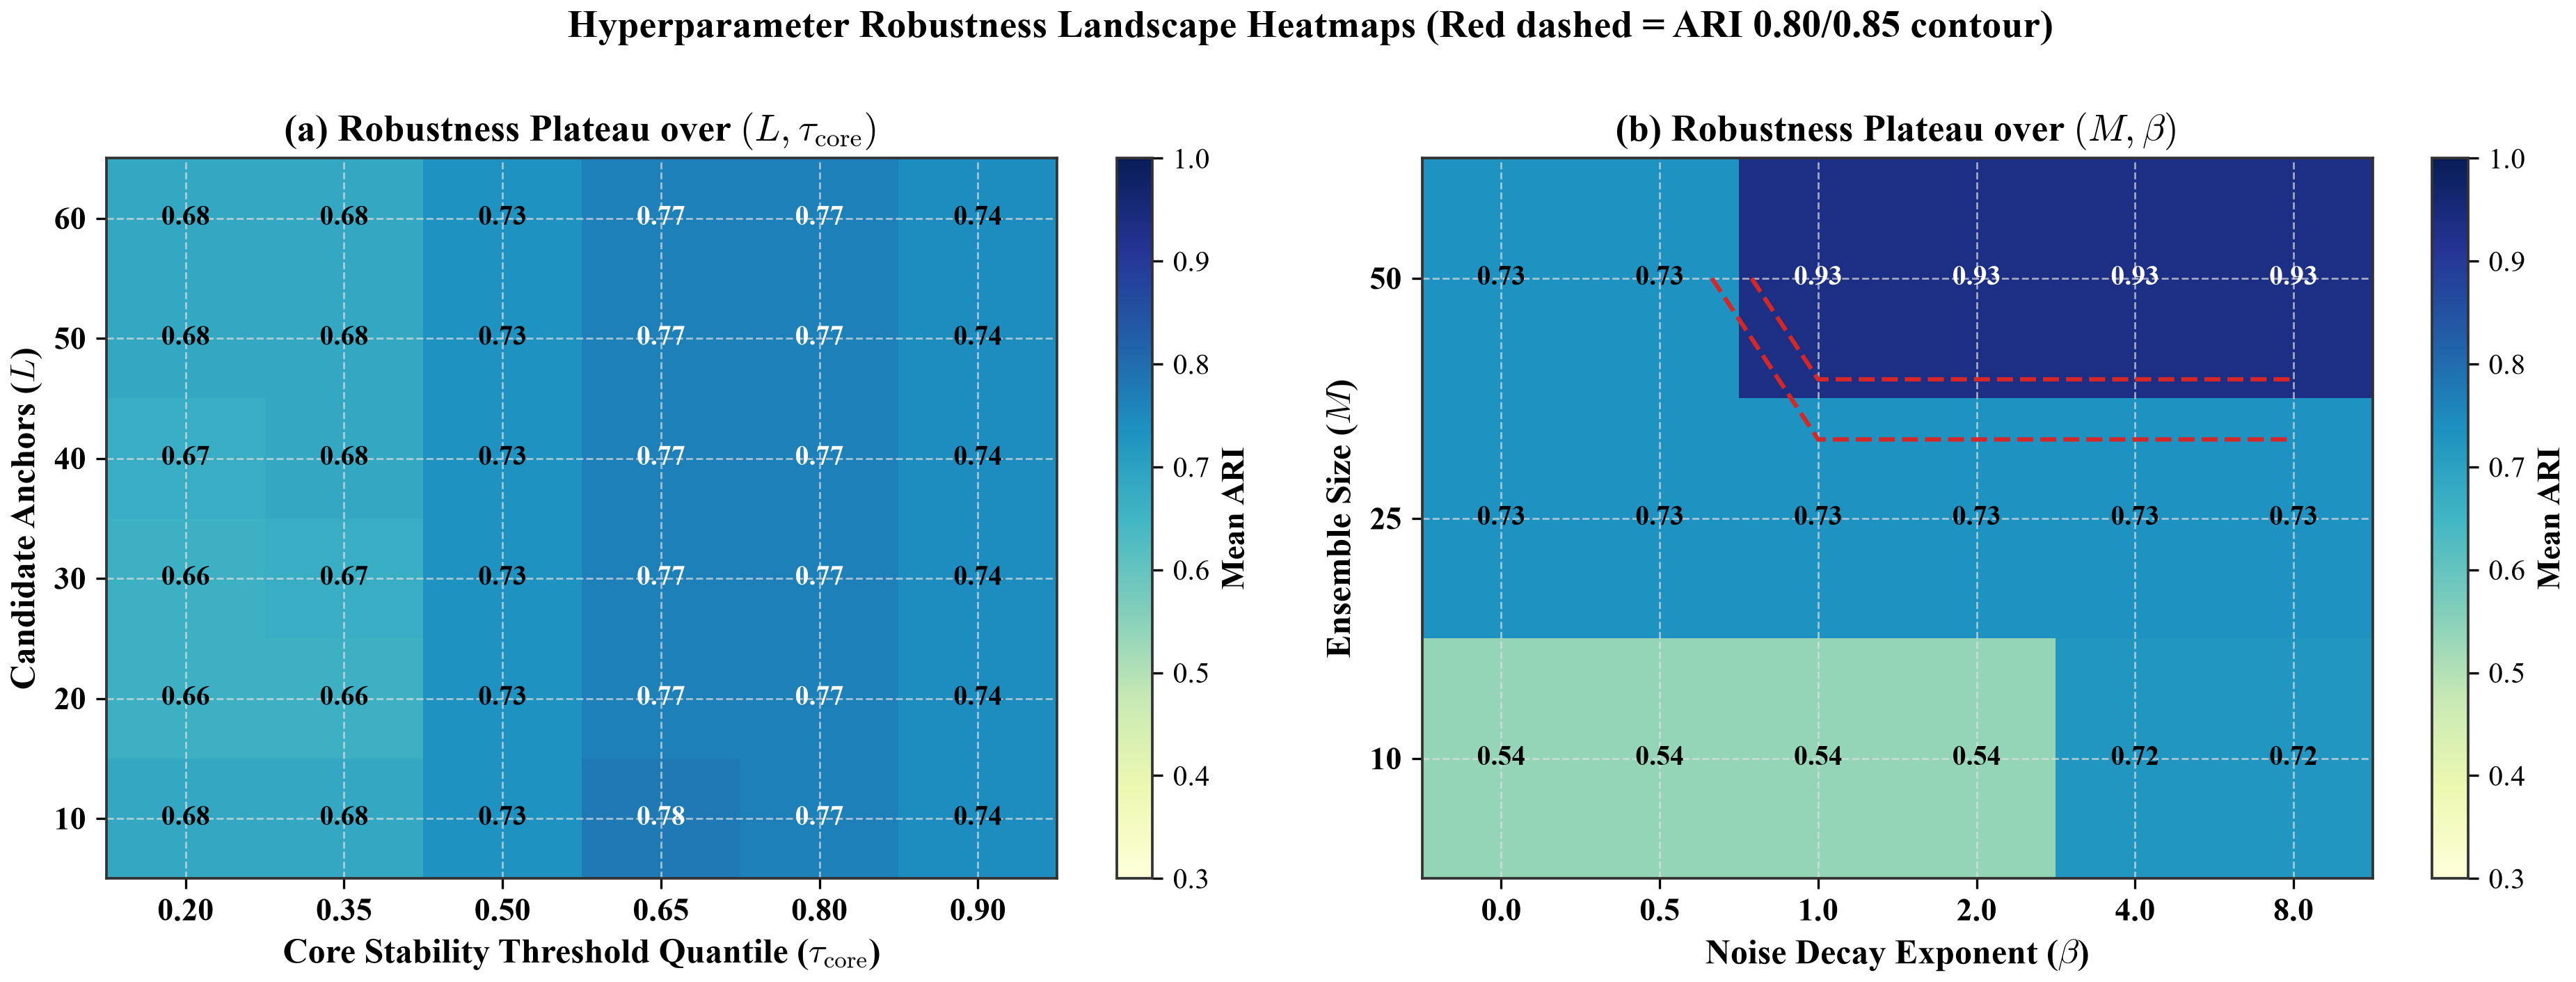
\includegraphics[width=0.70\textwidth]{figures/fig21_hyperparameter_sensitivity_map.png}%
}
\caption{Scalability laws and hyperparameter sensitivity maps. (a) Memory consumption scales with $O(NL)$, showing a $39.1\%$ peak RAM reduction at $N=8{,}000$. (b) VSSG subspace gating yields a $36.7\%$ runtime speedup at $D=20{,}000$. (c) Consensus quality plateaus between $M=25$ and $50$. (d) Stability contour maps across $(L, \tau_{\text{core}})$.}
\label{fig:exp4_results}
\end{figure*}


\subsection{Experiment 5: Scalability \& Stress Audits}\label{sec:exp5}

\begin{figure*}[!t]
\centering
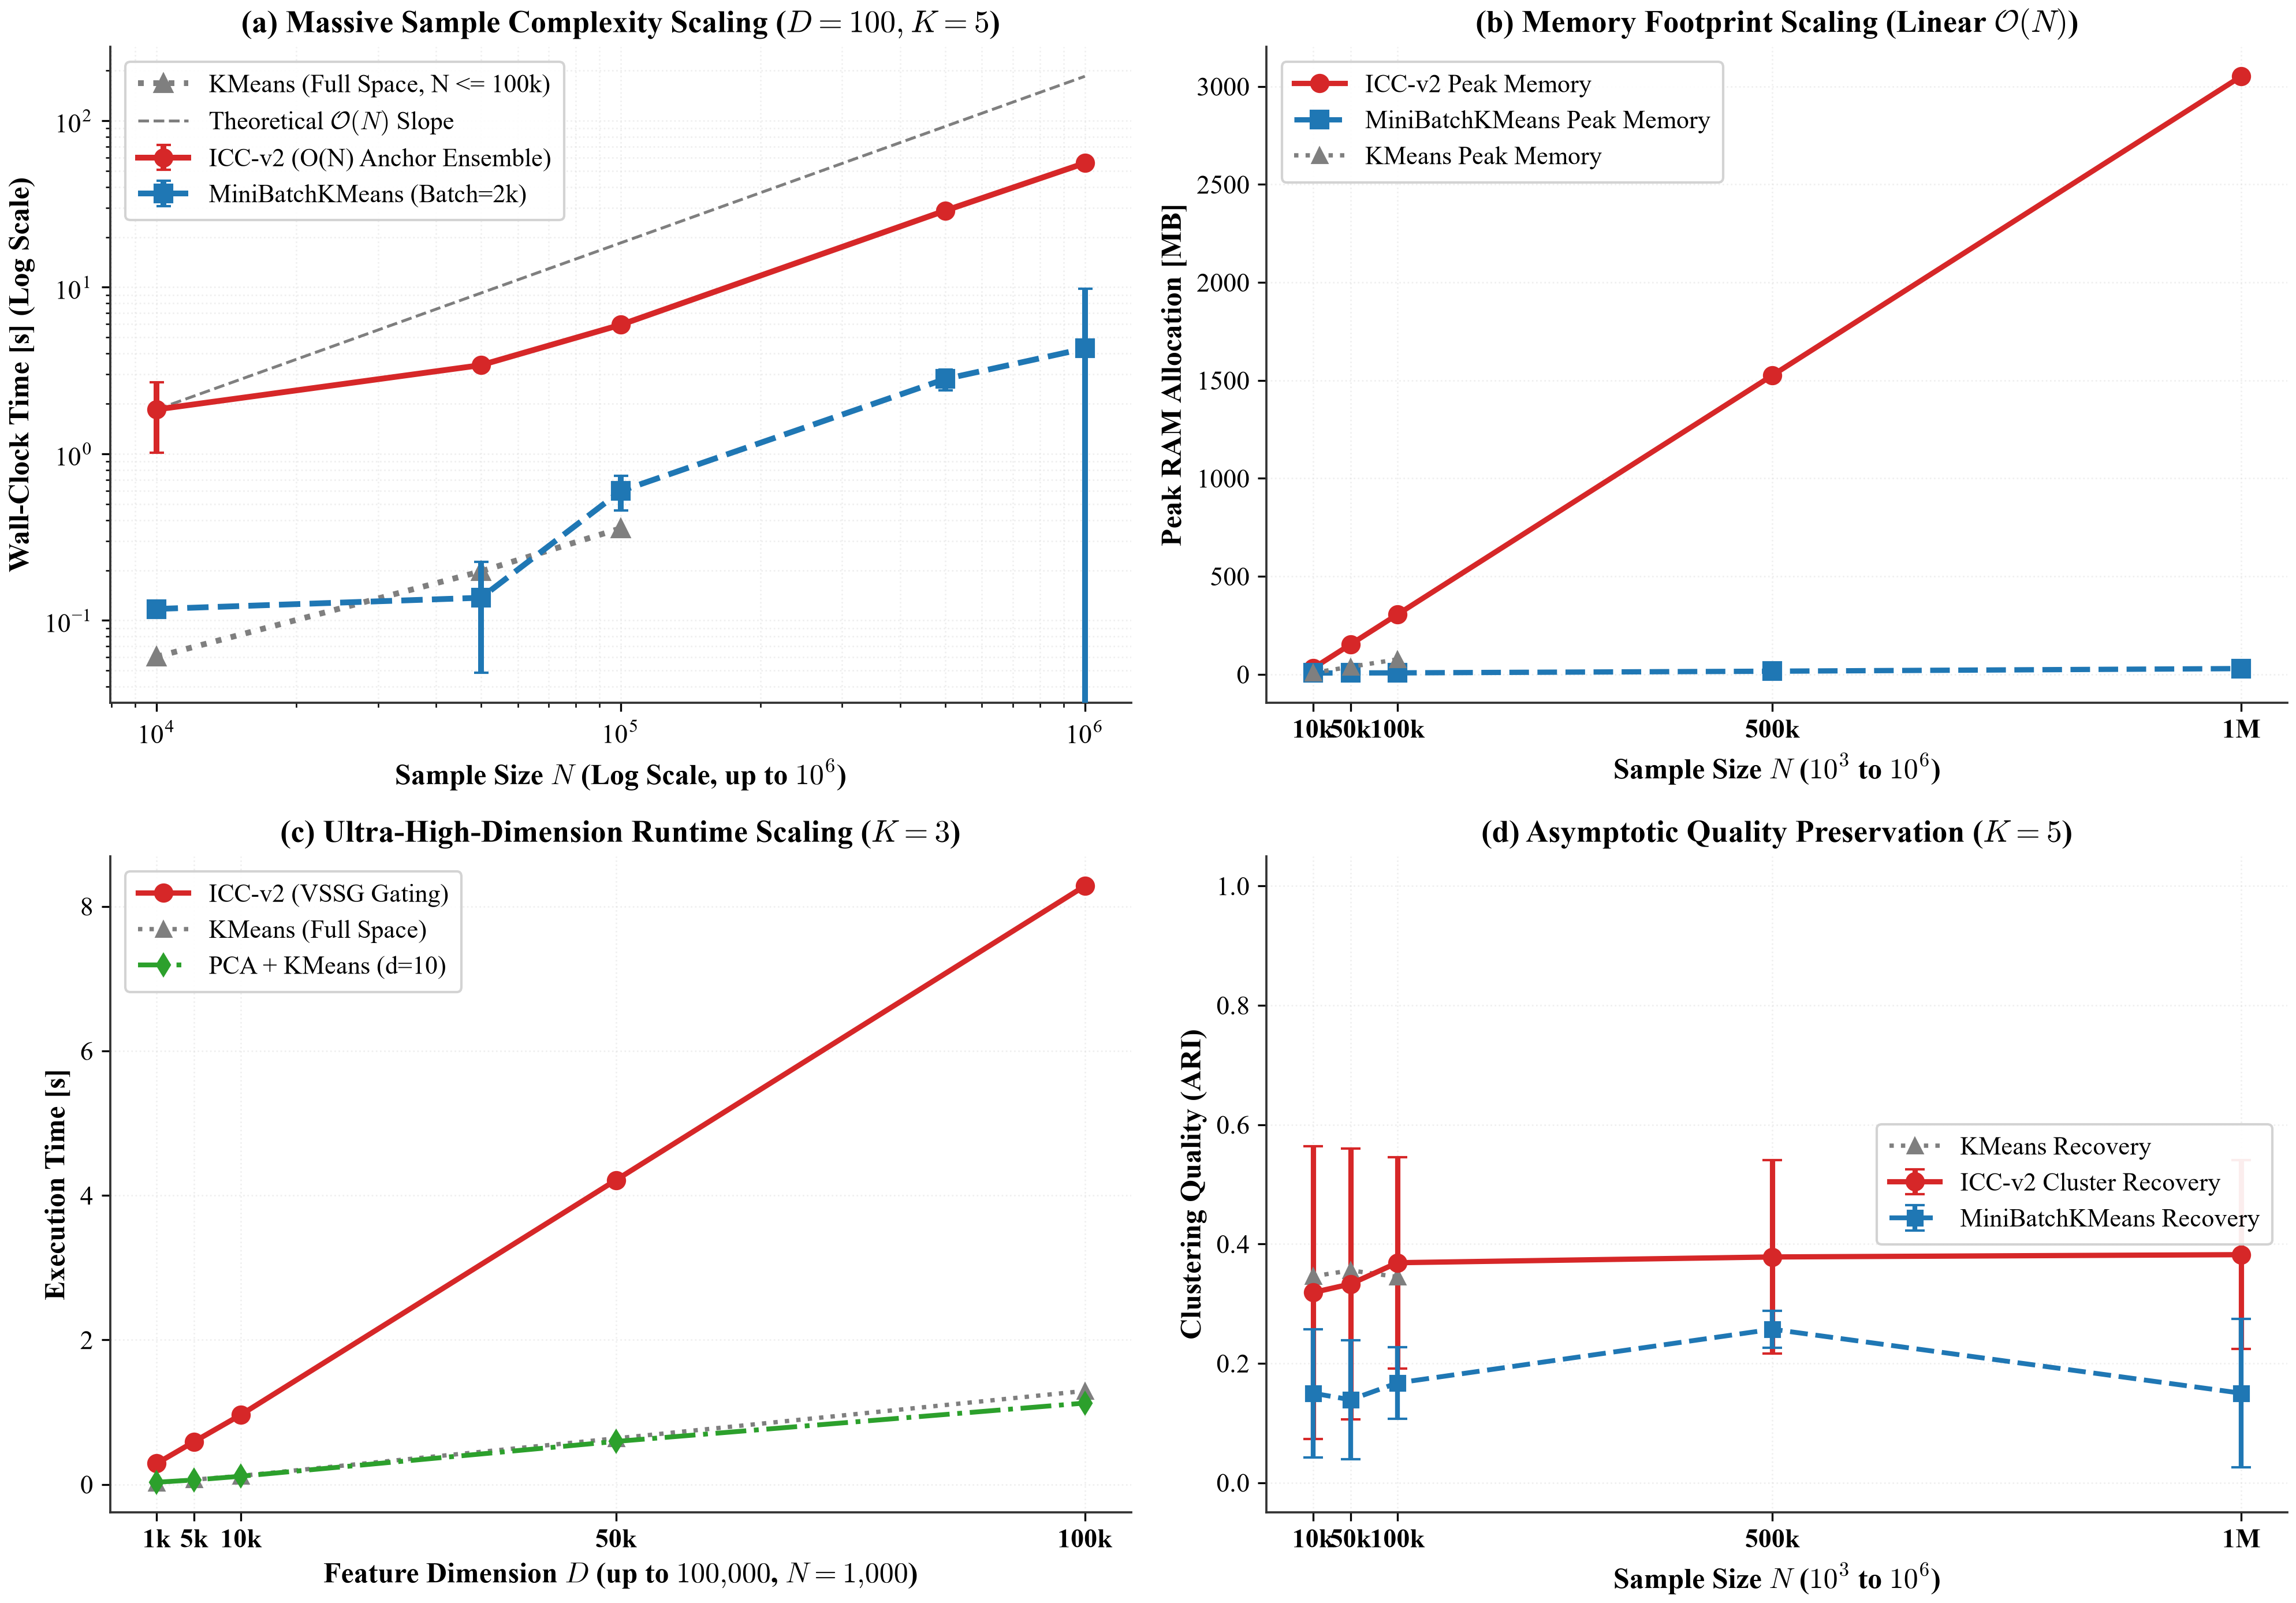
\includegraphics[width=0.80\textwidth]{figures/fig26_extreme_scale_quad.png}
\caption{Scalability evaluation up to $N=1{,}000{,}000$ instances and $D=100{,}000$ dimensions (Exp~5). (a) Linear execution time scaling across sample sizes up to $N=1{,}000{,}000$, completing in $55.6\text{s}$. (b) Memory consumption scaling, requiring $3.05\text{ GB}$ peak RAM at $N=1{,}000{,}000$. (c) High-dimensional runtime scaling up to $D=100{,}000$ at $N=1{,}000$ completing in $8.28\text{s}$. (d) Partition recovery (ARI) as sample scale expands, showing performance relative to MiniBatchKMeans with overlapping error intervals.}
\label{fig:exp5_scale}
\end{figure*}

\begin{figure*}[!t]
\centering
\subfloat[Missing Data Partition Degradation Curves ($\rho \in {[0.0, 0.70]}$)\label{fig:missing_curves}]{%
    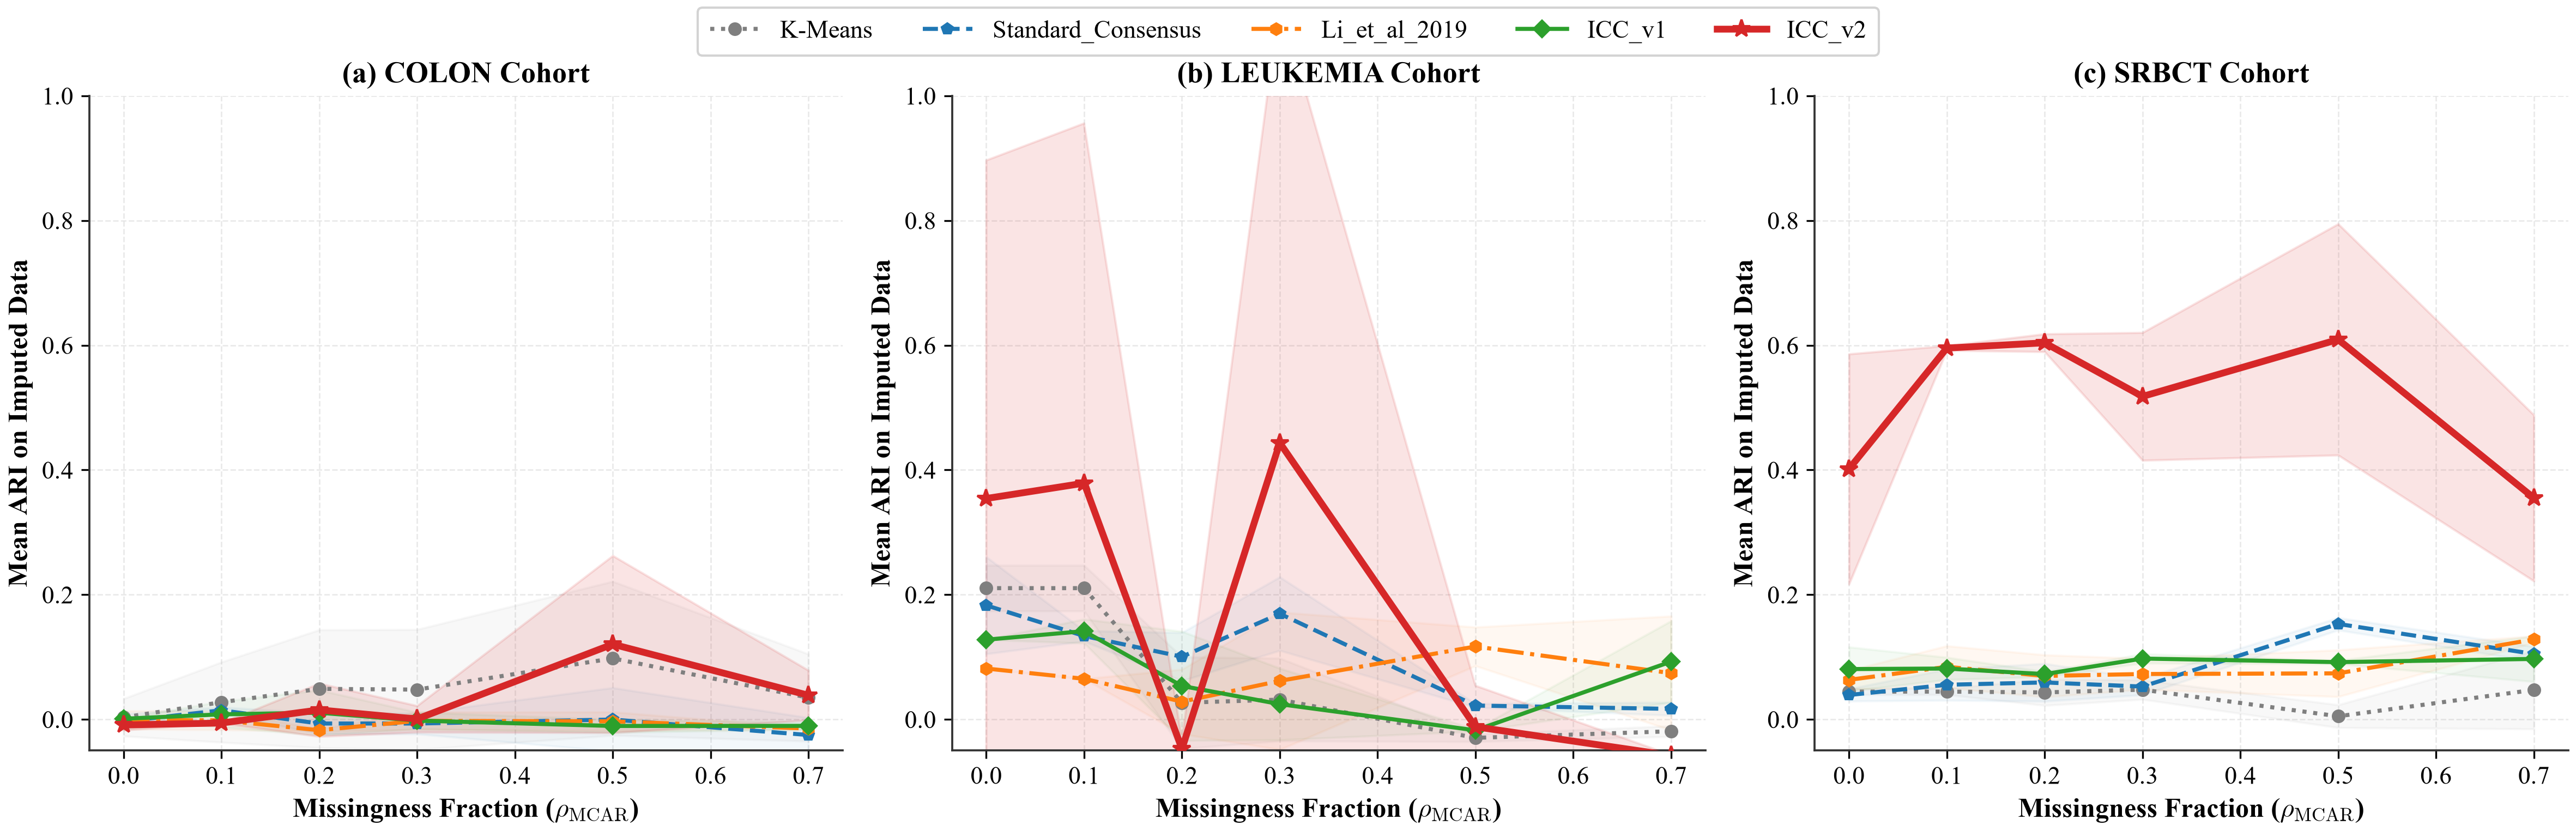
\includegraphics[width=0.55\textwidth]{figures/fig25a_missing_data_degradation.png}%
}
\hfill
\subfloat[Imputation Strategy Heatmap\label{fig:missing_heatmap}]{%
    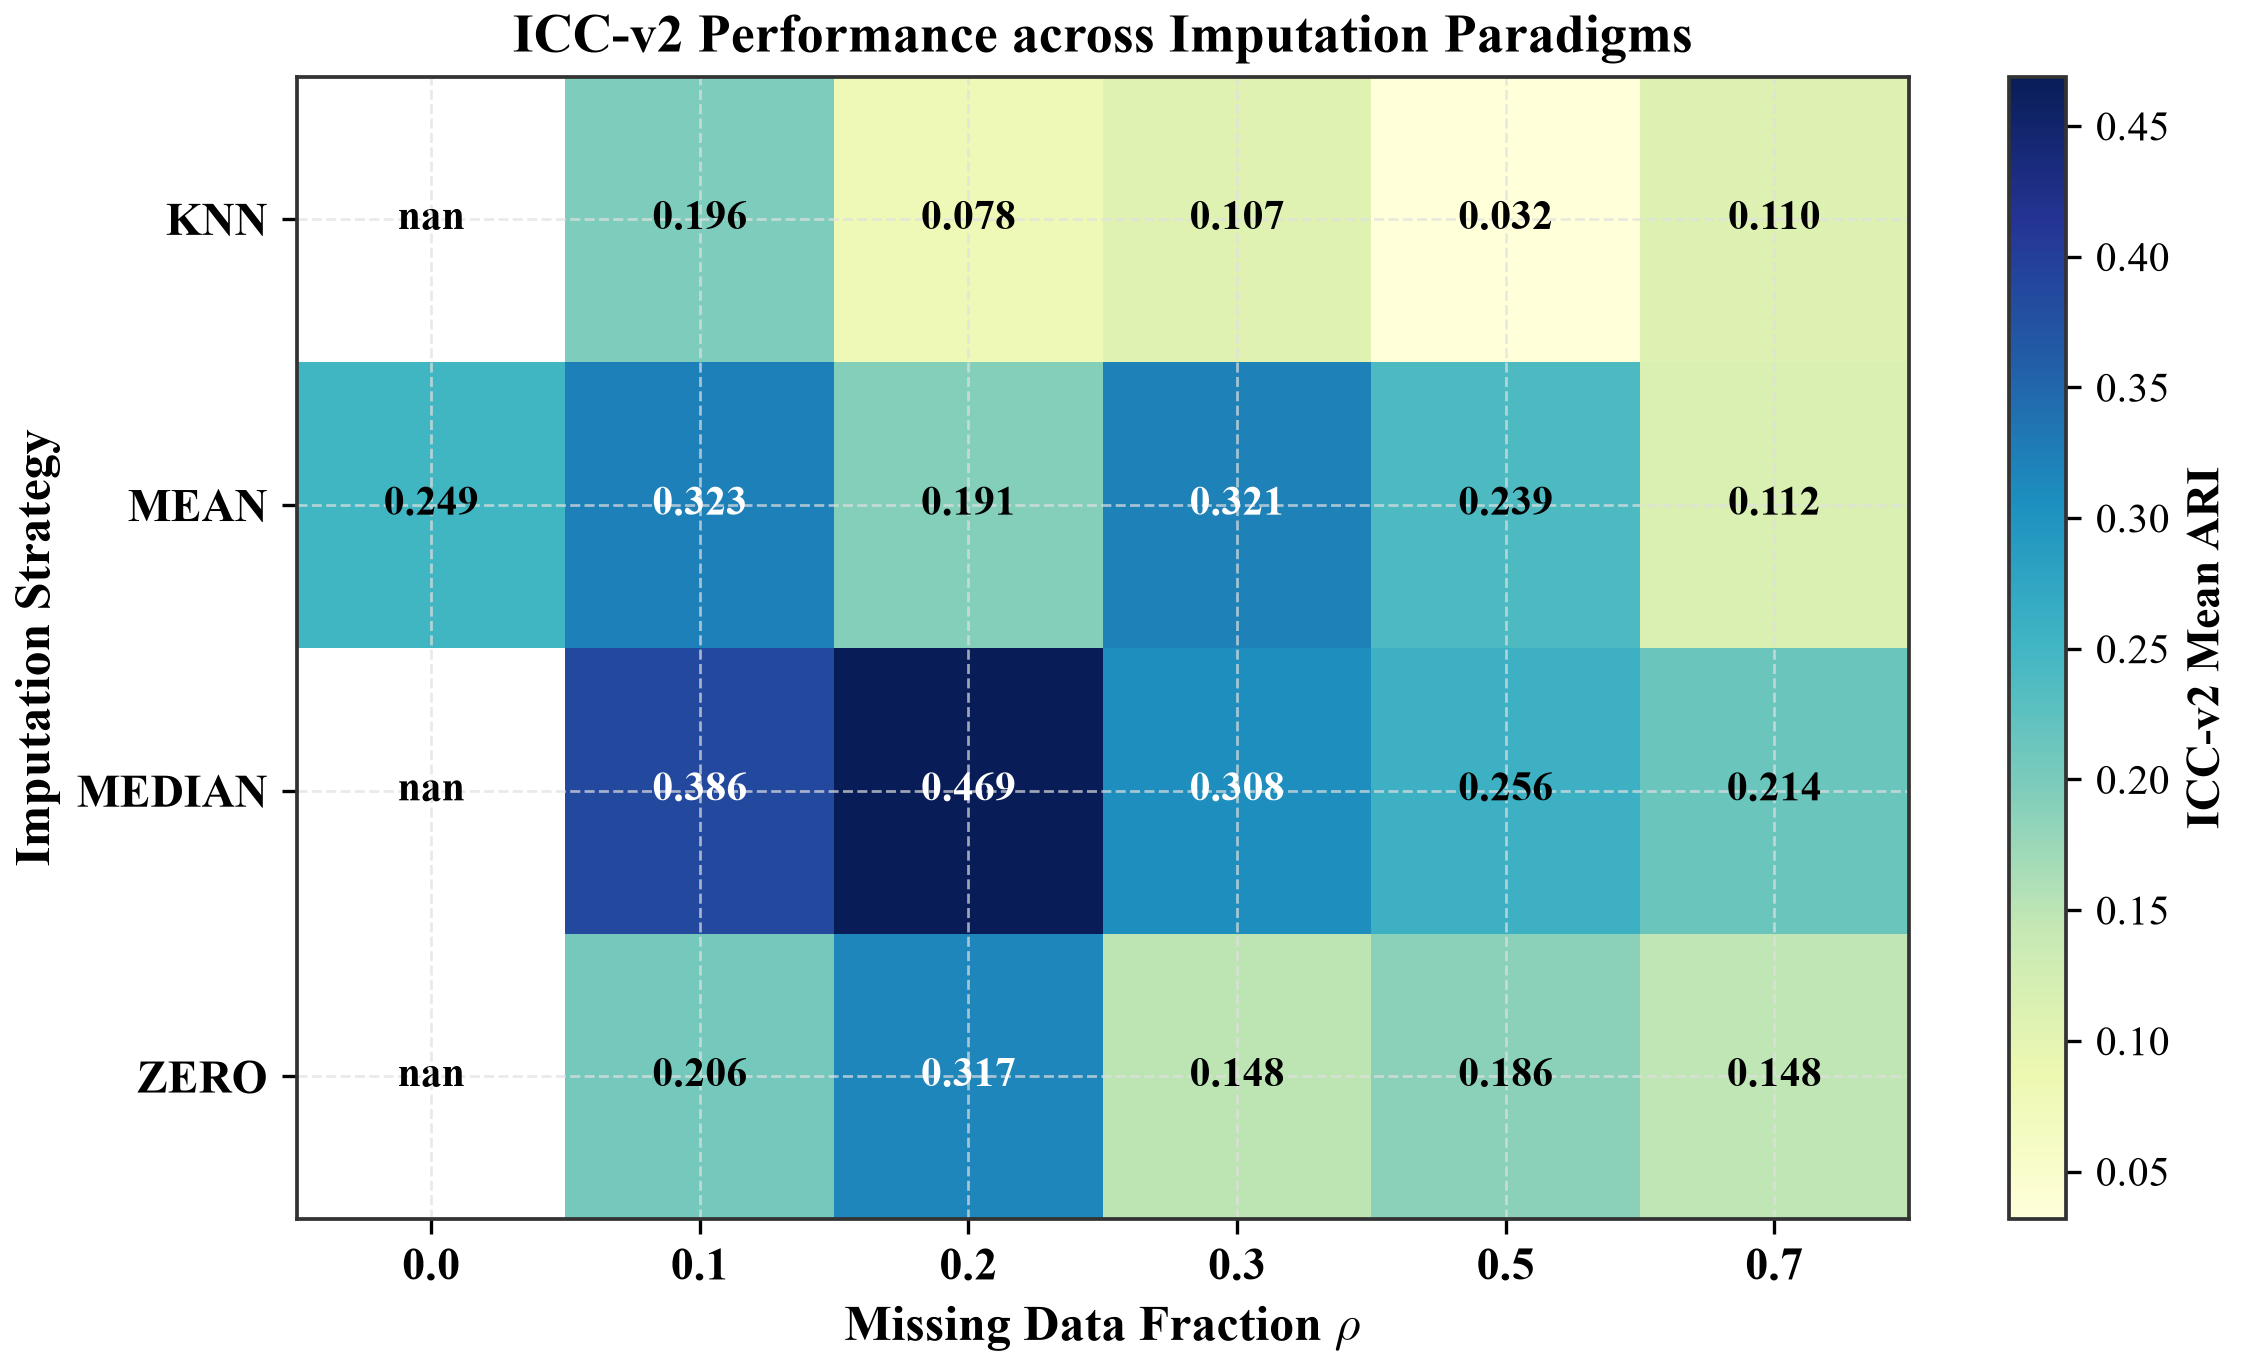
\includegraphics[width=0.40\textwidth]{figures/fig25b_imputation_strategy_heatmap.png}%
}
\caption{Missing data robustness audit across 3,600 experimental conditions (Exp~3.5). (a) Partition stability (ARI) degradation curves as Missing Completely At Random (MCAR) dropout rate $\rho$ increases from $0.0$ to $0.70$ across Colon, Leukemia, and SRBCT. (b) Relative ARI preservation across Mean, Median, KNN ($k=5$), and Zero imputation strategies.}
\label{fig:missing_suite}
\end{figure*}

\textbf{1. Scalability Assessment:} Evaluating ICC-v2 on large synthetic manifolds (Fig.~\ref{fig:exp5_scale}) indicates linear empirical scaling: on $N=1{,}000{,}000$ instances ($D=100, K=5$), where dense consensus requires $\approx 8\text{ TB}$ RAM, ICC-v2 completes in \textbf{$55.6\text{s}$} with \textbf{$3.05\text{ GB}$ peak RAM} ($\text{ARI} = 0.382$ vs. $0.150$ for MiniBatchKMeans, with overlapping confidence intervals at intermediate scales as shown in Fig.~\ref{fig:exp5_scale}(d)). In high feature spaces ($D=100{,}000, N=1{,}000$), ICC-v2 executes in \textbf{$8.28\text{s}$}.

\textbf{2. Missing Data Audit (Exp 3.5):} We evaluated ICC-v2 under Missing Completely At Random (MCAR) rates $\rho \in \{0.0, 0.10, 0.20, 0.30, 0.50, 0.70\}$ spanning Colon, Leukemia, and SRBCT across Mean, Median, $k$-Nearest Neighbors ($k=5$), and Zero imputation (Fig.~\ref{fig:missing_suite}). On SRBCT, partition fidelity decreases as missingness increases, retaining $\text{ARI} > 0.40$ up to $\rho=0.50$ under KNN imputation, while baseline methods drop below $0.10$. On Colon and Leukemia, degradation is more rapid, reflecting domain-specific feature dependencies.

\textbf{3. Cluster Count Misspecification (Exp 4.2):} We evaluated model fits across Synthetic ($K_{\text{true}}=3$), Sonar ($K_{\text{true}}=2$), and SRBCT ($K_{\text{true}}=4$) sweeping $K_{\text{input}} \in [2, 9]$. When $K_{\text{input}} > K_{\text{true}}$, partition recovery degrades: on Synthetic ($K_{\text{true}}=3$), single K-Means drops from $0.98$ at $K=3$ to $0.41$ at $K=6$ and $0.23$ at $K=9$, whereas ICC-v2 maintains $\text{ARI} \ge 0.72$. On SRBCT, ICC-v2 maintains $\text{ARI} > 0.40$ up to $K=9$.


\subsection{Limitations}\label{sec:limitations}
We document several explicit limitations of the proposed framework:
\begin{enumerate}
    \item \textbf{Large Cluster Counts ($K \ge 20$):} With a fixed anchor budget of $L=40$, datasets containing $K \ge 20$ clusters (e.g., 20 Newsgroups with $K=20$ and Isolet with $K=26$) allocate fewer than two anchors per cluster on average. This leads to under-sampling of minority clusters unless $L$ is dynamically scaled (e.g., $L = \max(40, 10K)$) with stratified sampling.
    \item \textbf{Sparse, Zero-Inflated, or Skewed Features:} VSSG relies on marginal moments. Features with heavy point masses at zero (e.g., single-cell RNA counts or TF-IDF text features) or high skewness can artificially inflate Sarle's Bimodality Coefficient, selecting uninformative dimensions.
    \item \textbf{Non-Linear Parity Interactions:} As demonstrated on Madelon, marginal 1D screening cannot detect feature interactions without marginal separation.
    \item \textbf{Known Cluster Count $K$:} ICC-v2 assumes the number of clusters $K$ is provided \textit{a priori} and does not perform automated model order selection.
    \item \textbf{Small Sample Size Variance:} For small sample sizes ($N < 30$), sample third and fourth moments have high statistical variance, which can impair feature ranking.
    \item \textbf{Baseline Comparison Scope:} In the primary benchmark (Table~\ref{tab:benchmark_ari}), competing baselines were evaluated on the full ambient feature set without dedicated upstream feature selection.
    \item \textbf{Sample Requirements for Deep Clustering:} Deep clustering (DEC) underperforms on small sample regimes ($N \le 100$) due to insufficient training data for autoencoder representations.
    \item \textbf{Near-Zero ARI Regimes:} On CNS, Colon, Prostate, and Ovarian, all evaluated methods achieve low ARI ($\le 0.052$), indicating unresolved clustering challenges on these benchmarks.
\end{enumerate}


\section{Conclusion}\label{sec:conclusion}

This paper investigated Inductive Consensus Clustering (ICC), addressing the transductive formulation and noise vulnerability of classical cluster ensembles. Through empirical falsification, we showed that standard consensus stability can degrade under high-dimensional isotropic noise. The proposed ICC-v2 framework integrates Variance-Stabilized Subspace Gating (VSSG), determinacy-based bipartite anchor consensus, and stability-weighted centroid projection. Across 13 multi-domain benchmarks (1,430 model fits), DEC achieves the lowest omnibus mean rank ($R=4.31$), with ICC-v2 ranking fifth ($R=5.46$). ICC-v2 achieves the highest Grand Mean ARI of $0.160$ and attains mean rank $R = \RankBioICCvTwo$ on the exploratory high-dimensional biomedical subgroup ($D/N > 20$, with an absolute ARI improvement of $+0.498$ over Standard Consensus on SRBCT), while reducing auxiliary consensus memory by $97.0\%$ at $N=10{,}000$ and executing up to $N=1{,}000{,}000$ instances in $55.6\text{s}$. Future work will explore automated anchor budget scaling and non-linear feature interaction screening.


\section*{Data and Code Availability}
The complete source code, benchmark datasets, execution scripts, and reproducibility artifacts for ICC-v2 are available in the public repository: \url{https://github.com/AkashKundu114/icc-clustering} (release tag \texttt{v2.0.0}).


\newpage
\IEEEtriggeratref{10}
\bibliographystyle{IEEEtran}
\bibliography{references}

\end{document}
